This chapter first describes the two datasets MS COCO and 3Dshapes used in this work. Then, the agents' architecture is presented. There are two agents---the speaker and the listener agents---whose architectures are shared across all experiments. Finally, the single experiments and their results are discussed. The chapter is closed with a general discussion of language drift results in these experiments.

\section{Datasets}

This work uses two datasets for the reference game. The dataset chosen for the main experiments is the MS COCO Captions dataset \parencite{chen2015microsoft}. As it is one of the most widely used image datasets containing real photos of common objects and scenes, this choice was motivated by the goal of this work to test multi-agent communication on natural images annotated with natural language captions. 

Further, a second dataset was chosen for conducting baseline experiments in order to investigate potential sources of language drift---the 3Dshapes dataset developed by \textcite{burgess20183d}. This dataset was chosen due to its systematic content and exhaustive annotations of all relevant image features, allowing to automatically generate exhaustive natural language captions for the dataset. This dataset has by far less features and categories varying across the images compared to the main dataset, providing a baseline for estimating the models' performance in a more controlled environment.

Both datasets are used for constructing the reference game which procedes in the following way:
\begin{enumerate}
	\item A random image is sampled from the dataset as the target $t$.
	\item A second image is sampled as the distractor $d$ (either at random or following constraints; see below for details).
	\item The speaker agent $S$ receives both images, the target image being marked, respectively. This is accomplished by always passing the target as the first image. It emits a message $m$ describing the target.
	\item The listener agent $L$ receives both images in randomized order along with the message $m$, but doesn't know which image is the target.
	\item The listener selects the target image based on the message. If the selection was correct, both agents receive a positive reward, and a negative one otherwise.	 
\end{enumerate}

The next two sections describe in detail the properties of the datasets and how they were preprocessed for the experiments.

\subsection{MS COCO}
\label{ds:coco}
The MS COCO Captions dataset \parencite{chen2015microsoft} contains images and respective annotations from the 2014 split of the MS COCO dataset \parencite{lin2014microsoft}. Figure \ref{fig:coco_example} presents an example image and annotations form the dataset. The dataset contains 82,783 images in the training split, each associated with around five human-annoated caption, resulting in a total of 414,113 unique image-caption pairs. The validation split contains 40,504 images, annotated with a total of 202,654 human-produced captions. The respective dataset splits and annotations were downloaded from \url{https://cocodataset.org/#download}.
Furthermore, each image is annotated with bounding boxes of objects and category labels for the depicted objects. There are 80 different basic-level annotation categories, listed in the Appendix \ref{appendix}. These 80 categories are grouped into 12 superordinate categories (see Tab.~\ref{tab:app_coco_categories}).
On average, 2.9 basic-level categories and 2.3 superordinate categories occur per image.

The natural language captions associated with the images contain a total of 24,697 unique tokens. Yet over 99\% of the words occuring in the entire dataset are covered by 6000 most frequent tokens. 
The final size of the vocabulary $V$ used in the experiments is 4054, including four special tokens \texttt{START, END, UNK, PAD}, as it comprises over 98\% of the token distribution mass, while comprising 16.4\% of unique tokens occurring in all captions. This vocabulary size was chosen as a good trade-off between a sufficient variety of words that the speaker can choose to describe the images and an action space size which is still learnabale in the current set-up. 

The minimal caption length occuring in the dataset is six tokens, the maximal length is 57 tokens. The mean caption length is 11.3 tokens (based on tokenization with the basic English tokenizer provided by the \texttt{torchtext} package). Since recurrent neural networks may have issues with learning very long sequences \parencite[e. g.,][]{jaeger2002tutorial}, captions exceeding the length of 15 tokens were truncated. This cut-off length was chosen because it is the minimal length at which over 99\% of the captions didn't have to be truncated. %\pt{maybe include a density plot, side by side with the vocab count density one}
During preprocessing, the captions were lowercased, tokenized with the \texttt{torchtext} tokenizer mentioned above and tokens were mapped to numerical indices. The resulting vocabulary is shared between the speaker and listener agents in all experiments. 

The following preprocessing steps were applied to all images before training: the images were resized to 256 pixels, random $224\times224$ pixel crops were taken, images were horizontally flipped with a probability of 0.5 in order to increase the speaker's viewpoint invariance and each RGB channel was normalized using values expected by the pretrained ResNet50 module \parencite{he2016deep}.

For the baseline experiments, the training pairs of images were sampled at random. In contrast, for the experiment involving similar training pairs the images were sampled such that the distractor depicted objects similar to the target. This was controlled via the category annotations accompanying each image. These annotations comprise basic-level category labels and their respective superordinate categories (see Appendix \ref{appendix}) for the bounding boxes for objects in the images provided with the dataset.
The training pairs were constructed so that they were annotated with at least three same basic-level categories (i..e, at least three same category objects occurred in both images). In case there were less than three object annotations in the image, a distractor was chosen that matched on the one or two remaining annotated categories.

\subsection{3Dshapes}
\label{ds:3dshapes}
The 3Dshapes dataset introduced by \textcite{burgess20183d} contains 480.000 synthetically generated images. These images depict different three-dimensional geometric objects in abstract space, systematically varying along six different features. These features are the color of the ground on which the object resides (ten values), the color of the background walls (ten values), the color of the object itself (ten values), the type of object (four values), its size (eight values) and its position within the depicted room (15 values). %\pt{Table X depicts / describes the possible values of each dimension}. 
The $64\times64$ pixel images are labeled with six-dimensional vectors, each position representing the value of one of the six features.
The dataset was downloaded from \url{https://storage.cloud.google.com/3d-shapes/3dshapes.h5}.
\begin{figure}
\centering
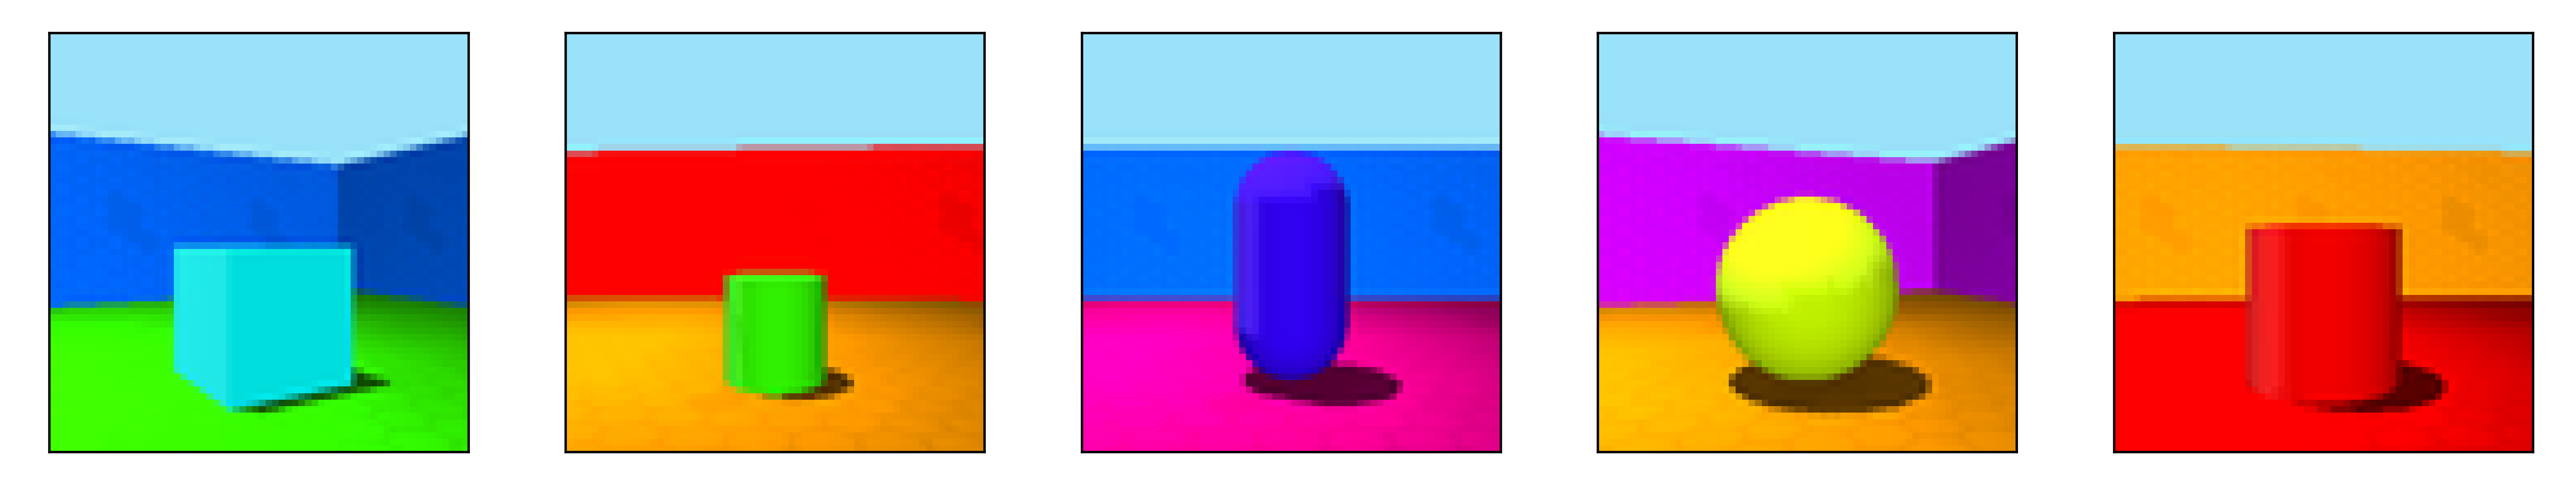
\includegraphics[width=\linewidth]{images/3dshapes_example.png}
\caption{Example images from the 3Dshapes dataset. Examples of corresponding generated captions (from left to right): ``A big cyan block in the right corner on green floor in front of a medium blue wall.''; ``The green cylinder in the middle in front of a red wall on orange floor is tiny.''; ``A middle-sized dark blue pill located in the middle in front of a medium blue wall on pink floor.''; ``The picture shows a huge yellow ball on orange floor in front of a purple wall close to the right side.''; ``The large cylinder on red floor in front of a orange wall in the middle is red.''.}
\label{fig:3dshapes_example}
\end{figure}  

\subsubsection{Caption Generation}

The dataset provides symbolic feature labels of the images. However, since the goal of presented work is training artificial agents to use natural language in communication, English captions were generated for this dataset. More specifically, two datasets were generated. 

The first dataset is tailored towards studying the effect of including maximally exhaustive image descriptions in the training data. Therefore, generated captions include natural language descriptions of all six features and their values, appearing in different syntactic constructions. Figure~\ref{fig:3dshapes_example} shows example images along with sample generated captions. The syntactic variations were introduced in order to avoid potential effects of order in which descriptions of certain features might occur.
The captions were generated by constructing generation rules and sampling all possible resulting sentences using the \texttt{nltk} package \parencite{bird2006nltk}. The resulting dataset contains 20 synonymous captions per image, five of which are sampled at random for training in order to match the MS COCO conditions. The captions were build using a vocabulary of 49 tokens. Maximal caption length is 25 tokens, the minimal length is 16 and mean caption length is 18.9 tokens. 

The second dataset provides the comparison for investigating the role of having exhaustive captions compared to including shorter less comprehensive captions on the same dataset. That is, the exhaustivity manipulation is done on the same visual input, while keeping constant the vocabulary size. This dataset contains \textit{non-}exhaustive captions which only mention two to three out of six features of each image. These captions were generated using the same procedure. 27 captions per image were generated. The maximal caption length in this dataset is 13 tokens, the minimal is three tokens and the average length is 7.2 tokens.
The same examples along with non-exhaustive captions can be seen in Fig.~\ref{fig:3dshapes_example_short}.
The comparability of the vocabulary sizes is important in that it determines the difficulty of learning the policy for a given action space (which \emph{is} the vocabulary in case of communication) with REINFORCE which represents the functional learning in these experiments \parencite[cf.][]{havrylov2017emergence}.

The generation rules and the corresponding code can be accessed under \url{https://github.com/polina-tsvilodub/3dshapes-language}.

\begin{figure}
	\centering
	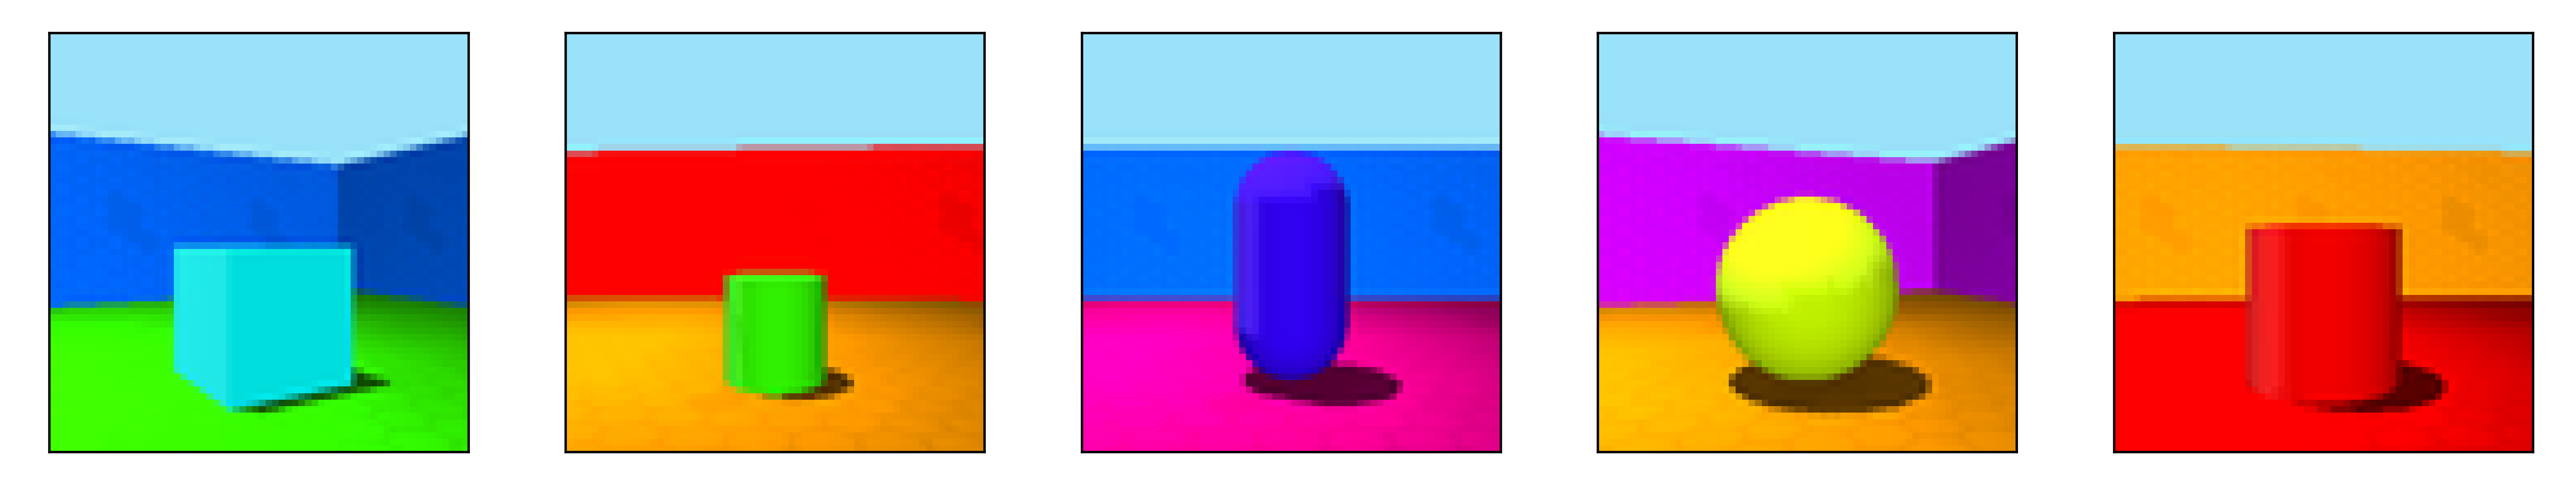
\includegraphics[width=\linewidth]{images/3dshapes_example.png}
	\caption{Example images from the 3Dshapes dataset. Examples of corresponding generated captions (from left to right): ``The block is in front of a medium blue wall.''; ``A tiny cylinder.''; ``There is a pill in the middle.''; ``A yellow ball close to the right side.''; ``A red cylinder in front of a orange wall.''.}
	\label{fig:3dshapes_example_short}
\end{figure} 

Akin to MS COCO experiments, baseline experiments were conducted on random target-distractor pairs. For the similar pairs experiments, the distractor was chosen so that it matched the target with respect to at least three out of six features. For instance, if the target depicted a tiny red cube in the left corner on yellow floor and with blue background, the distractor could depict a tiny blue cube in the right corner on yellow floor and with green background.

%This dataset was chosen due to the systematicity of its content , allowing to generate natural language captions for each image which would exhaustively describe all features of the images. Since no such captions exist to the author's knowldege, they are generated as part of this thesis. To this end, a base context-free grammar (CFG) containing production rules for captions was manually created. The syntactic rules were constructed on the basis of examples of captions created by the author for samples from the dataset. Each caption must contain descriptions of all six feature dimensions. The terminal production rules mapping the pre-terminal to natural language labels are chosen for each image based on its unique feature value configuration. For each image, \pt{X captions are sampled from all the possible productions allowed by the grammar}.


\section{Architecture}
\label{architecture}
The architecture of the agents follows \textcite{lazaridou2020multi}, except minor details to be explained below. As described in Chapter \ref{chapter03}, \textcite{lazaridou2020multi} explore different ways to parametrize the speaker agent, and the current work replicates the ``multi-task learning'' parametrization (p.~5). This choice is motivated by the fact that among their architectures, this is the only one where the speaker agent learns to produce messages and its core image captioning capability while having access to both the target and the distractors, as opposed to models relying on sampling captions from a pretrained single-image captioning models. The chosen architecture is used in all experiments.

Both agents have two components: a visual embedding module which takes as input the target and distractor images, and a language module. More specifically, the visual module for both agents embeds image features which were extracted using the same pre-trained ResNet50 model \parencite{he2016deep}. The weights were accessed through the \texttt{torchvision.models} API \parencite{marcel2010torchvision}. Features from all training images of the dataset were extracted and saved and then retrieved when training all agents. 
The language module differs for the two agents, so details are provided below. 
The code for all experiments can be found under \url{https://github.com/polina-tsvilodub/mSc-thesis}. 

\subsection{Speaker}
The speaker receives as input tuples \texttt{(targets, distractors)}, where \texttt{targets} as well as \texttt{distractors} are features extracted from the ResNet50 for the sampled pairs, respectively. That is, the speaker knows which of the the two images in a given iteration of the reference game is the target for which the message should be produced. The speaker then produces a probability distribution over vocabulary tokens of the message given the input $P(m \mid i_t, i_d)$, parametrized by the speaker model parameters $\theta_S$. From a reinforcement learning perspective, training the speaker amounts to estimating the parametrized speaker policy $\pi_{\theta_s}(m \mid i_t, i_d)$.

The speaker model consists of a linear layer which projects the 2048-dimensional image features to 512-dimensional embedding space. The linear layer is first applied to both the target images and then to the distractors, resulting in embeddings $i_t$ and $i_d$, respectively. The vectors are concatenated to $[i_t; i_d]$, the target embeddings always being the first ones, such that the speaker network implicitly knows which features represent the target. These 1024-dimensional vectors are used as additional context in the speaker's language module. The core of the module is the recurrent Long Short-Term Memory (LSTM) cell \parencite{hochreiter1997long}. More specifically, the language module consists of three layers: an embedding layer, mapping the vocabulary to 512-dimensional word embeddings, a one-layer LSTM with 512-dimensional hidden and cell states; and a linear layer on top, mapping the last hidden state of the LSTM to a distribution over the vocabulary. The size of the vocabulary depends on the dataset (see above).

During the reference game training, the speaker receives pairs of images, embeds them and prepends the concatenated embedding to the special \texttt{START} token. This 1536-dimensional embedding is then passed through the LSTM and the linear output layer. The next token is sampled from a categorical distribution parametrized with the probabilities computed from the hidden state in the previous timestep. The sampled token is concatenated with the image embeddings and input to the next timestep. This procedure repeats until the \texttt{END} token is sampled or the maximum caption length is achieved. The \textit{baseline} experiments use the pure decoding strategy described above; additional experiments investigate the effects of using greedy decoding (Section~\ref{expt:coco_greedy}). This architecture is also a common practice in image captioning literature (cf. Chapter \ref{chapter02}). Another possible approach that could be explored in future work would be to initialize the hidden states of the LSTM with the visual embeddings. In this case, the hidden and cell states of the LSTM were initialized with random values sampled from the standard normal distribution.The embedding and last linear layers' weights were initialized with random values sampled from the uniform distribution between -0.1 and 0.1, the biases were initialized with zeroes.  
This architecure results in a total of 9,402,838 trainable parameters (for a vocabulary  size of 4054) or a total of 5,297,713 parameters (for a vocabulary of 49 tokens).  %\pt{Make a graphic of the models and / or the reference game}.

\subsection{Listener}
The listener receives as input the tuples \texttt{(images1, images2, messages)}, the first two inputs being ResNet50 features of the image pairs, input in random order, such that the agent doesn't know which image is the target. The \texttt{message} is the caption produced by the speaker. The listener then produces scores $P(i|m)$ over images identifying which one is the target, parametrized by the listener model parameters $\theta_L$.

The message is passed to the language module which consists of an embedding layer, mapping the vocabulary to 512-dimensional word embeddings, and a one-layer LSTM with 512-dimensional hidden and cell states. All weights are initialized analogously to the respective weights of the speaker model. The hidden cell state $h_i$ at the last time step of embedding the received message is used as the final message representation. 
The visual module of the listener consists of a linear layer which also projects the 2048-dimensional image features to a 512-dimensional embedding space. The images are passed through the linear layer one after the other, resulting in embeddings $i_1$ and $i_2$. Finally, the listener computes dot products between each image embedding and the message embedding. The dot products are used to parametrize a categorical distribution over the image indices; the target is then sampled from this distribution.  
The architecture results in 1,049,088 trainable parameters for the listener's visual module and 4,176,896 (for 4054 tokens) trainable parameters for its LSTM (2,126,336 parameters for 49 tokens).


\subsection{General Training Details}
\label{general_train_details}
All experiments were trained with a batch size of 64 pairs, using the Adam optimizer with a learning rate  of 0.001 \parencite{kingma2014adam}. In the reference game setting, due to computational constraints, the models were trained for two epochs per experiment. \footnote{Pretraining and some experiments were conducted on a MacBook Pro with four Intel cores i7-1068NG7 with CPU @ 2.30GHz. On average, pretraining took 2h/epoch, reference games took 6h/epoch. Remaining experiments were conducted using Google Colab and their Tesla P100 GPU with 16GB memory. There, training took on average 3h/epoch.} 

In the reference games, following \cite{lazaridou2020multi}, the speaker parameters $\theta_S$ were updated by optimizing a compound loss function $J_s$. More precisely, the speaker loss consisted of a weighted sum of a functional loss $L_f$ and a structural loss $L_s$. The former was computed via the REINFORCE rule based on the listener's task performance (i.e., referential success). The speaker received the reward 1 if the listener guessed the target successfully, and -1 otherwise. The structural loss was a supervised training loss, computed via cross-entropy between the message produced by the speaker and the ground truth caption for the given target image. $L_f$ additionally included an entropy regularization term, weighted by 0.1. The resulting loss was:
\begin{equation}
J_s = (1-\lambda_s)L_f + \lambda_s L_s
\end{equation}
In particular, the structural loss weight $\lambda_s$ was varied in some experiments in order to address \textbf{H4}.
The listener parameters $\theta_L$ were updated via cross-entropy loss $J_l$ optimized based on the guessed target index compared to the ground truth targets. 

\subsubsection{Hypotheses Operationalization}
Given the experimental architecture reported above, this section describes more specific operationalizations of some hypotheses about the language drift which may occur in the experiments, presented in Section \ref{hypos}.\\
\newline
\textbf{H1}--\textbf{H3}, \textbf{H6}, \textbf{H9}--\textbf{H10} concern structural and semantic drifts, relative to functional improvement of the agents (i.e., the speaker's functional loss improvement and listener's task accuracy increase). The former is operationalized as decreasing log probability of the speaker's message under a pretrained language model. The latter is operationalized as decreasing conditional log probability of the speaker's message given the target image, under the pretrained speaker model. \newline
\textbf{H4:} Given that the pressure to stay close to a natural language distribution is provided by the structural loss component in the models, it is expected that both the structural and the semantic drifts increase as the weight of the structural loss component decreases. To investigate this, five reference games with the structural loss weights $\lambda_s \in \{0, 0.25, 0.5, 0.75, 1\}$ were conducted. The functional loss component was computed as $\lambda_f = 1 - \lambda_s$, respectively. That is, the drifts were expected to increase as $\lambda_s$ approached 0.\newline
\textbf{H5:} The discriminativity of the captions is expected to increase less in the similar target-distractor pairs experiment than in the baseline experiment on random pairs. That is, the overlap values are expected to be smaller than in the baseline experiment due to the higher perceptual and referential difficulty of discriminating images depicting similar things. 

\section{Experiment Procedures and Results}

This section first provides an overview of speaker pretraining, before zooming in on conducted experiments and discussing their procedures as well as results with respect to the described hypotheses.
First, a general pipeline of the main reference games as it applies to all experiments described below is provided.

\subsubsection{General Procedure}
\begin{enumerate}
	\item Speaker and potentially listener models are instantiated with pretrained weights. The experiment is configured with paramters like the decoding strategy, listener type, structural loss weight etc. (see experiments below for details).   
	\item Training image pairs are created from a set of 30,000 images and all five captions for each image unseen during pretraining, resulting in (approximately) 150,000 training pairs, batched into batches of 64 pairs. This results in 2343 training steps per epoch. The pairs are constructed either at random (while making sure the two images are not the same) or by choosing similar target-distractor pairs. 
	\item During each step, the agents play one reference game round: the speaker sees a target in context of a distractor and generates a messages about the target which is received by the listener. The listener sees the same images and picks the target based on the speaker's message. The speaker is updated according to both the structural well-formedness of her message compared to the ground truth caption of the target and the listener's success; the listener is updated according to her task success. 
	\item Each 200 steps of training, the structural and semantic drift metrics are computed on three held out batches (192 images) in order to observe their dynamics.
	\item After training, the agents are evaluated on a held out test set of 1,000 images which were neither part of pretraining nor of reference game training. During the evaluation, the agents are put in evaluation mode and the listener accuracy and all the drift metrics are computed. Depending on the evaluation, the 1,000 images are grouped into random or similar pairs. Generally, the drift values of the ground truth captions of the test sets and of the respective pretrained speaker captions on the test sets are treated as benchmarks for comparing drift dynamics.
\end{enumerate}
Specific configurations of each experiment are described in the respective sections. 

\subsection{Speaker Pretraining}
\label{speaker_pretraining}
\begin{figure}[h]
	\centering
	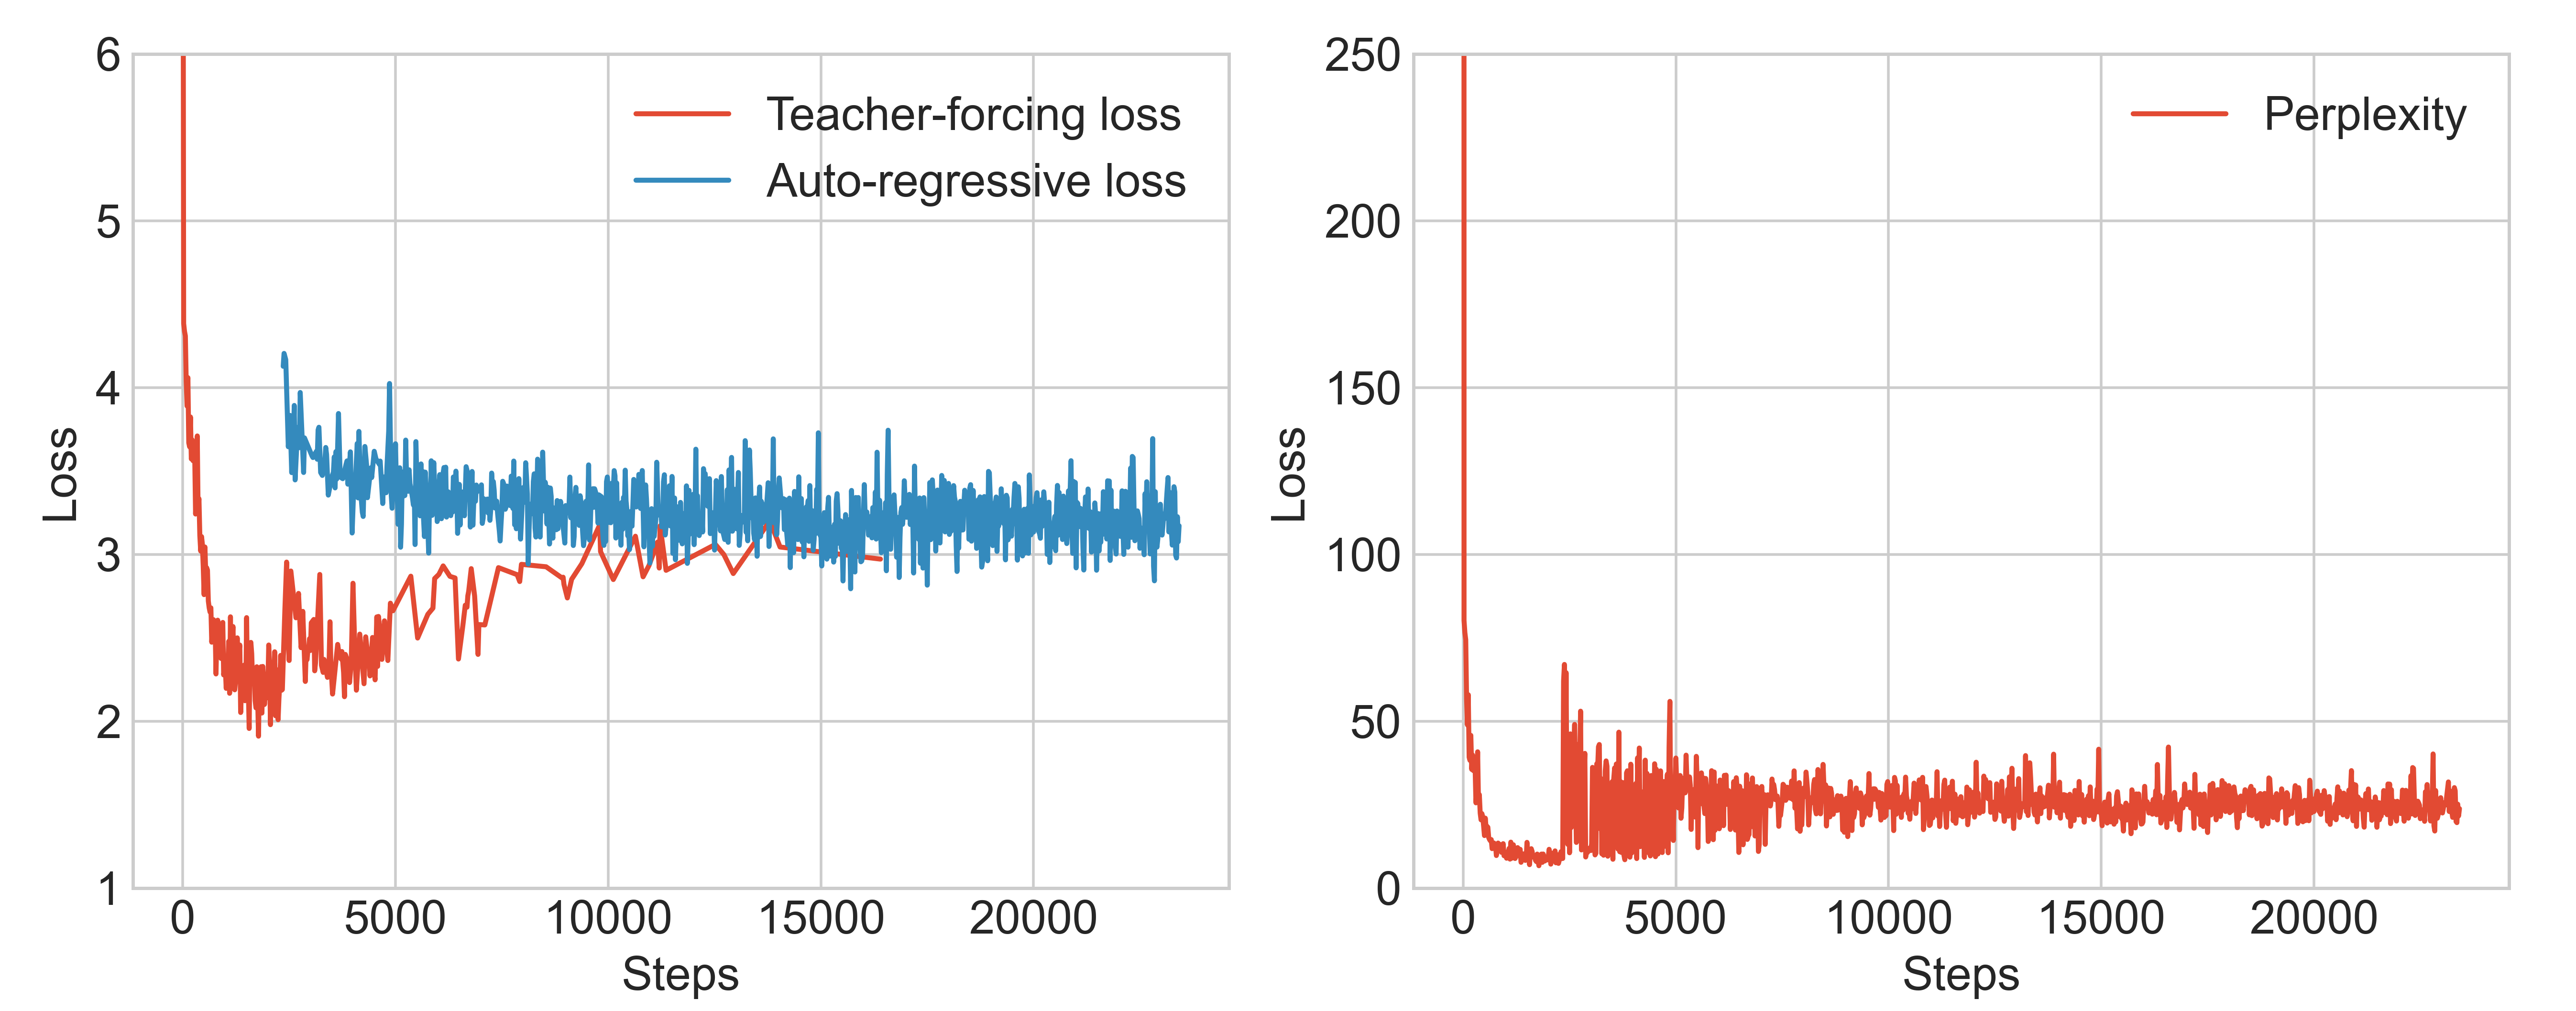
\includegraphics[width=\linewidth]{images/coco_pretraining_losses_ppls.png}
	\caption{Left: Training losses during pretraining the speaker on MS COCO; the colors indicate the pretraining mode, i.e., whether the ground truth caption (teacher-forcing loss, red) or the self-generated token (auto-regressive loss, blue) from the previous timestep was supplied at each timestep. Right: Training perplexity during pretraining of the speaker on MS COCO.}
	\label{fig:coco_pretraining}
\end{figure}  

\begin{figure}[h]
	\centering
	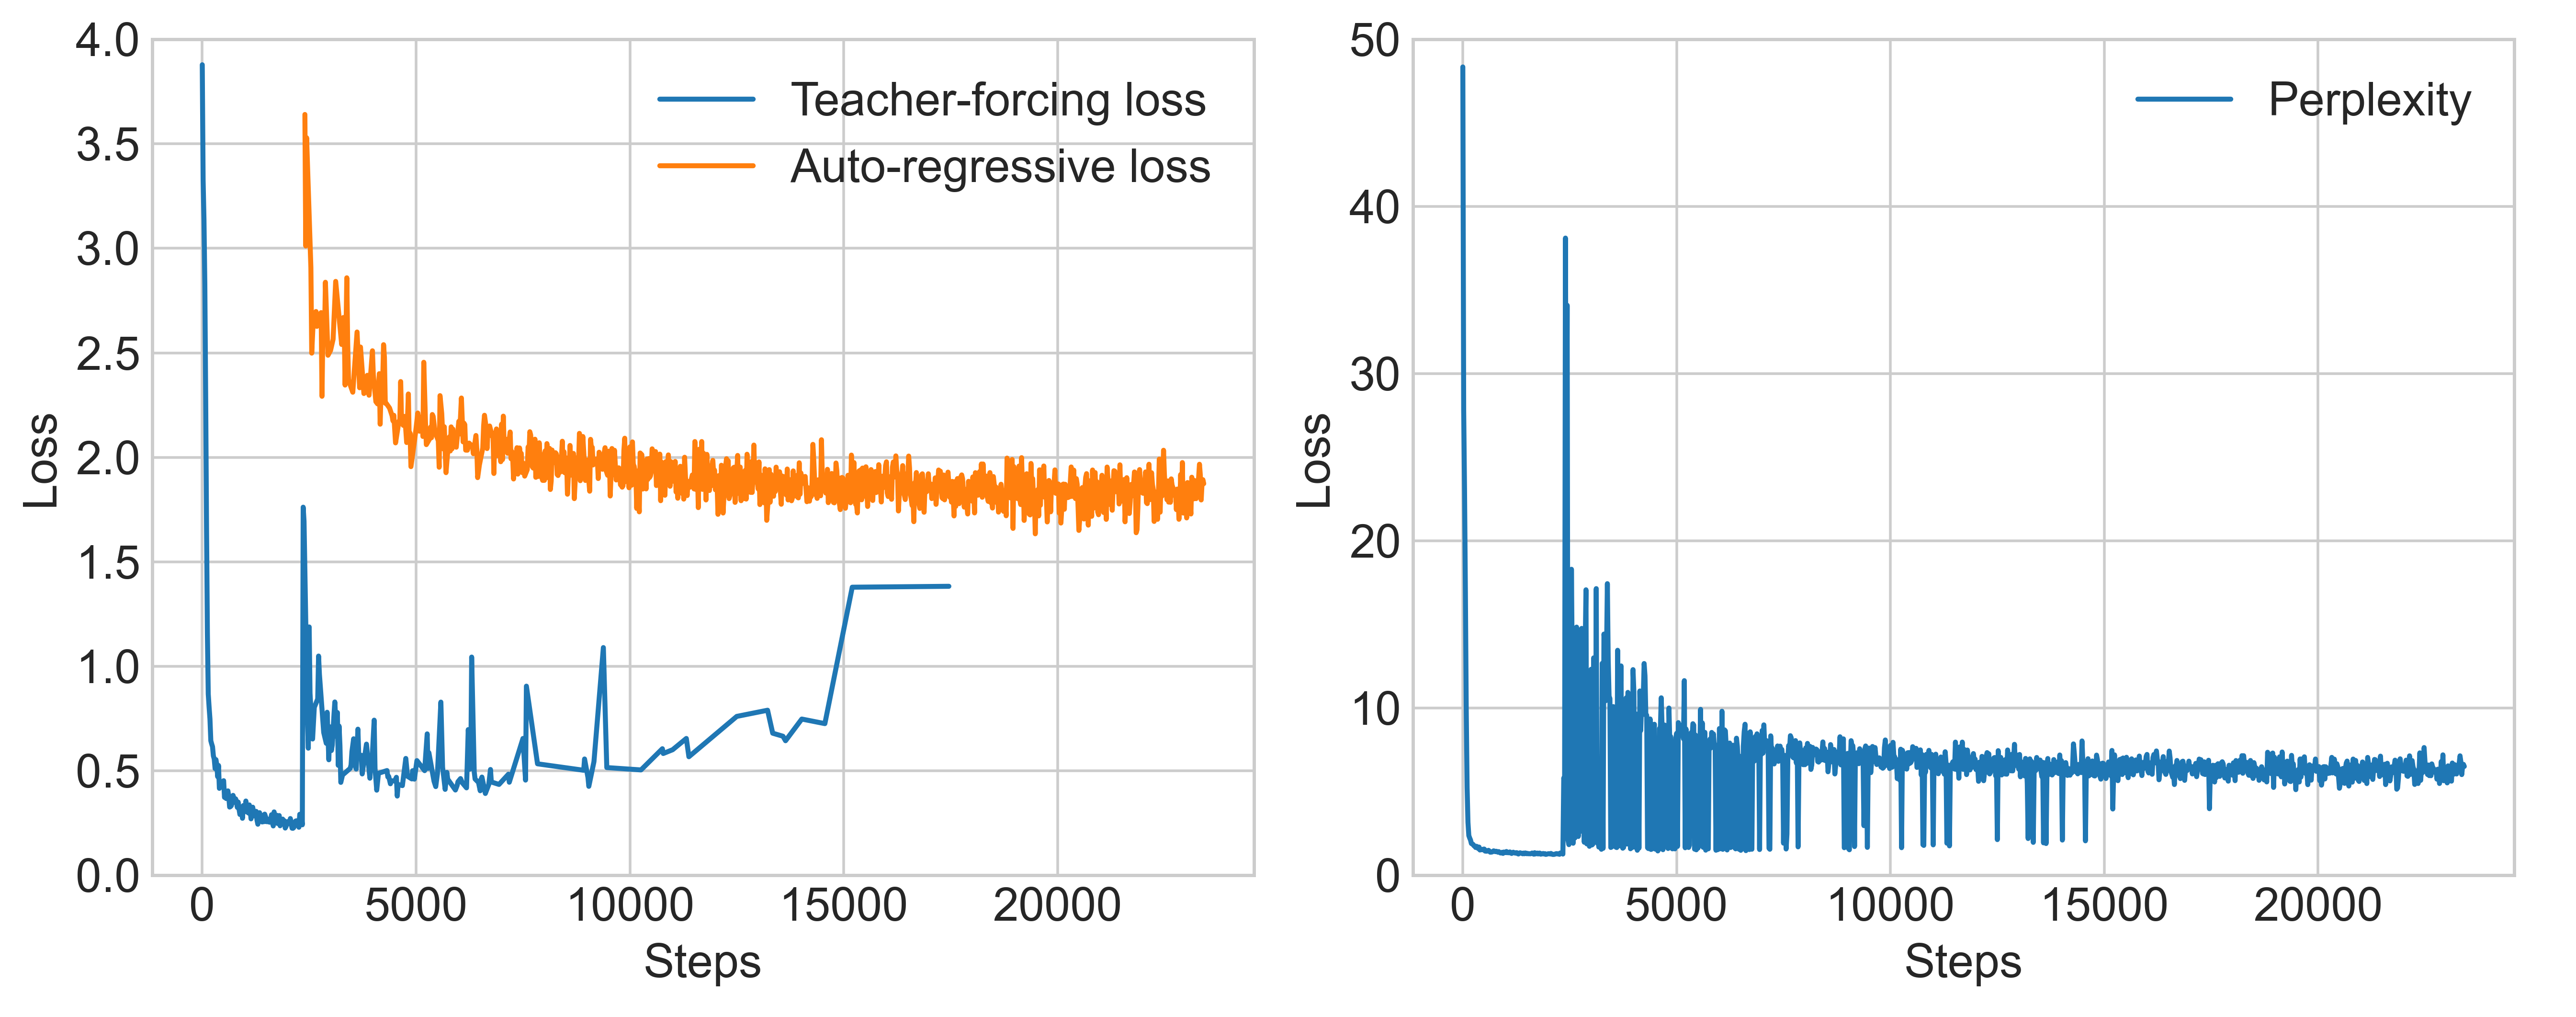
\includegraphics[width=\linewidth]{images/3dshapes_pretraining_losses_ppls.png}
	\caption{Left: Training losses during pretraining the speaker on the exhaustive 3Dshapes dataset; the colors indicate the pretraining mode, i.e., whether the ground truth caption (teacher-forcing loss, blue) or the self-generated token (auto-regressive loss, orange) from the previous timestep was supplied at each timestep. Right: Training perplexity during pretraining of the speaker on 3Dshapes.}
	\label{fig:3dshapes_pretraining}
\end{figure}  

\begin{figure}[h]
	\centering
	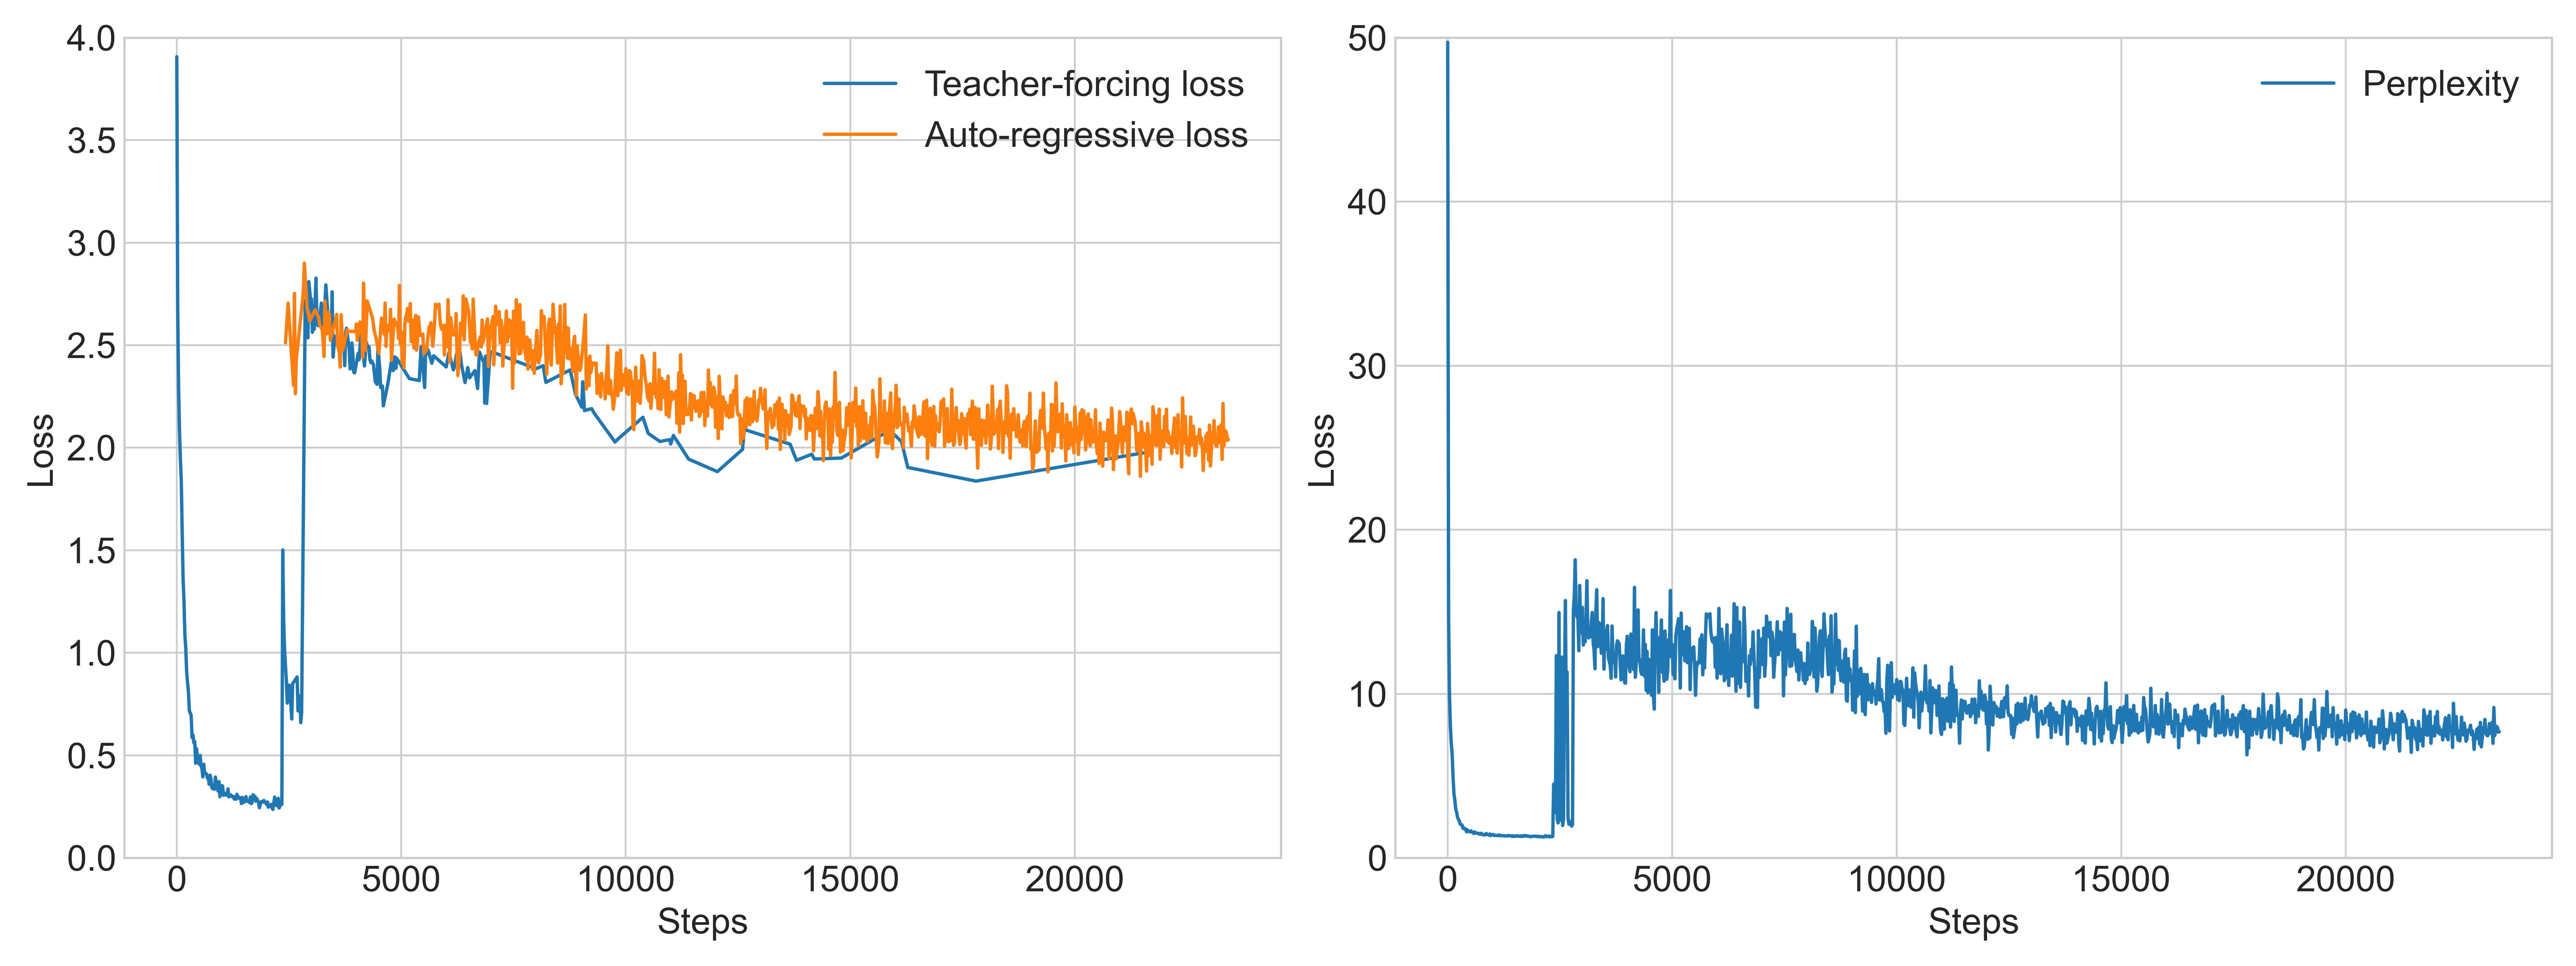
\includegraphics[width=\linewidth]{images/3dshapes_wShort_pretraining_losses_ppls.png}
	\caption{Left: Training losses during pretraining the speaker on the 3Dshapes dataset which includes both short and exhaustive captions; the colors indicate the pretraining mode, i.e., whether the ground truth caption (teacher-forcing loss, blue) or the self-generated token (auto-regressive loss, orange) from the previous timestep was supplied at each timestep. Right: Training perplexity during pretraining of the speaker on 3Dshapes.}
	\label{fig:3dshapes_pretraining_wShort}
\end{figure}  
%Table with image caption quality metrics of the pretrained speakers. Add same metrics of the speaker agents after ref games as rows to the same table. 

\begin{table}[]
	\begin{tabularx}{\textwidth}{|X|l|l|l|l|l|l|l|}
		\hline
		\textbf{Model name}                                    & \textbf{B-1} & \textbf{B-2} & \textbf{B-3} & \textbf{B-4} & \textbf{M} & \textbf{C} & \textbf{Val. loss} \\ \hline
		Pretrained MS speaker                             & 0.408           & 0.137           & 0.042           & 0.013           & 0.116           & 0.165          & 4.079                    \\ \hline
		MS Baseline, random, $\lambda_s = 0$      &   0.405              &      0.130           &     0.036            &     0.009            &     0.116            &     0.177           &           4.124               \\ \hline
		MS Baseline, random, $\lambda_s = 0.25$   &          0.413       &       0.134          &      0.041          &       0.015          &       0.116          &       0.189        &           4.074               \\ \hline
		MS Baseline, random, $\lambda_s = 0.5$   &          0.397       &       0.124          &      0.036          &       0.012          &       0.115          &       0.170         &           4.082               \\ \hline
		MS Baseline, random, $\lambda_s = 0.75$   & 0.407           & 0.133           & 0.037           & 0.010           & 0.116           & 0.178          & 4.056                    \\ \hline
		MS Baseline, random, $\lambda_s = 1$   &    0.405             &   0.125              &    0.033             &  0.000              &         0.115        &       0.181         &         4.066                 \\ \hline
		MS Baseline, random, similar pairs, $\lambda_s = 0.75$   &    0.292           &   0.066              &    0.010           &  0.000              &         0.068       &       0.018        &         4.180        \\ \hline
		MS Baseline, similar, random pairs  &     0.396            &          0.123       &       0.031         &        0.000         &   0.113         &      0.115          &      4.078                   \\ \hline
		MS Baseline, similar, similar pairs  &     0.299       &          0.066       &       0.000          &        0.000         &   0.068              &      0.018          &      4.235                    \\ \hline
		MS fixed listener, random, $\lambda_s = 0.75$  &        0.393         &       0.132          &        0.040         &      0.011           &      0.113           &        0.177        &       4.117                   \\ \hline
		Pretrained 3D speaker                            & 0.671           & 0.343           & 0.163           & 0.077           & 0.283           & 1.026          & 2.091                    \\ \hline
		3D Baseline, random, $\lambda_s = 0$     &                 &                 &                 &                 &                 &                &                          \\ \hline
		3D Baseline, random, $\lambda_s = 0.25$   &                 &                 &                 &                 &                 &                &          2.082                \\ \hline
		3D Baseline, random, $\lambda_s = 0.5$   &                 &                 &                 &                 &                 &                &         2.179                 \\ \hline
		3D Baseline, random, $\lambda_s = 0.75$  & 0.672           & 0.340           & 0.159           & 0.074           & 0.284           & 1.068          & 2.089                    \\ \hline
		3D Baseline, random, $\lambda_s = 1$   &                 &                 &                 &                 &                 &                &                          \\ \hline
		3D Baseline, similar, $\lambda_s = 0.75$ & 0.673           & 0.335           & 0.152           & 0.070           & 0.279           & 1.033          & 2.103                    \\ \hline
		\pt{FILL ME with more expts} &                 &                 &                 &                 &                 &                &                          \\ \hline
	\end{tabularx}
\caption{\label{tab:eval_metrics_refgame} Caption evaluation metrics and the validation loss on a heldout dataset, computed for the initial pretrained speakers and the speakers after training on the reference game. \textbf{B} denotes BLEU, \textbf{M} the METEOR score, \textbf{C} the CIDEr score, MS the MS COCO dataset and 3D the 3DShapes dataset. ``Baseline'' refers to the setup wherein the listener is trained jointly with the speaker, using pure decoding. ``Random'' refers to speakers trained on random target-distractor pairs; ``similar'' refers to speakers trained on similar target-distractor pairs.}
\end{table}

Before conducting reference games, the speaker agents were pretrained for both the MS COCO and 3Dshapes experiments. Conceptually, the model was pretrained in order to learn the statistical properties of English, i.e., ``learn to speak'', before being fine-tuned on the functional reference game task. This can be motivated as providing general \textit{task-unconditional} linguistic capabilities to the speaker which she can then transfer to specific tasks.

Both speakers were pretrained in a supervised fashion by sampling tuples of the form $(i_t, i_d, c_t)$ where $i_t, i_d$ were the target and distractor images, and $c_t$ was the target ground truth caption. The models were pretrained on 30,000 images selected at random from the respective dataset; for each image, the model saw five available ground truth captions. 
The pretraining was accomplished with the cross-entropy loss. Both models were trained for ten epochs.

As described in Section \ref{model_pretraining}, there are different strategies for pretraining the speaker. Based on initial exploratory experiments reported in Appendix \ref{app:grid_search}, all speakers were pretrained using an exponentially decreasing teacher-forcing rate $0.5^{epoch-1}$, transitioning to auto-regressive training with pure decoding. That is, in the auto-regressive mode the model was fed its own predicted token from the previous timestep during training; that token was generated by pure sampling. In teacher-forcing rounds, the ground truth tokens were fed instead.
Speakers for both datasets were pretrained in this set up. Figure \ref{fig:coco_pretraining} shows the pretraining dynamics of the MS COCO speaker, Figure \ref{fig:3dshapes_pretraining} shows the dynamics of the 3Dshapes speaker pretrained on exhaustive captions. Additionally, another 3Dshapes speaker was pretrained on both exhaustive and short captions from the second 3Dshapes annotations dataset. More precisely, for each image, five ground truth captions were selected, sampling at random whether three out of five captions were short or exhaustive. This additional speaker was trained for the experiments with short captions (addressing \textbf{H10}) in order to induce a bias towards actually generating short captions from pretraining; otherwise, without explicit pressure towards generating shorter messages, the speaker would be expected to produce exhaustive caption length messages \parencite[cf., e.~g.,][]{hupkes2020compositionality}. The pretraining results can be seen in Figure \ref{fig:3dshapes_pretraining_wShort}.

The evaluation of their image captioning capabilities on standard metrics (introduced in Chapter \ref{chapter02}) after pretraining can be found in Table \ref{tab:eval_metrics_refgame}. The metrics were computed on a held out validation split with 5000 unique images and respective captions. Comparing the pretrained speakers to state-of-the-art image captioning model peformance in Table \ref{tab_coco_metrics_ref}, it is apparent that the speakers perform somewhat worse in terms of standard caption evaluation metrics. It is hypothesized that this is due to the mixed teacher-forcing and auto-regression pretraining modes. It is conjectured that the speaker quality might only affect the absolute performance and drift metric values, but the qualitative comparisons between experiments will remain unaffected because all experiments are based on the same pretrained speakers.
Furthermore, all language drift metrics were computed for the pretrained models, presenting a baseline for linguistic capabilities, before any deterioration might take place due to task optimization (see Tables \ref{tab:coco_drift_metrics_basic}, \ref{tab:3dshapes_drift_metrics_basic_baseline}).

Equipped with the pretrained speaker agents, the reference game experiments are described below. First, main experiments on the MS COCO dataset are introduced. Then, the 3Dshapes experiments are presented.

\subsection{MS COCO: Baseline Experiments}
\label{expt:coco_baseline}

\begin{table}[]
	\begin{tabularx}{\textwidth}{|X|l|l|X|X|X|X|}
		\hline
		\textbf{Model name}                                    & \textbf{log $P(m)$} & \textbf{log $P(m \mid i)$} & \textbf{Overlap (d)} & \textbf{Overlap (c)} & \textbf{Acc. (random)} & \textbf{Acc. (similar)} \\ \hline
		Ground truth val.               &     -108.566            &          -80.399             &    9.147           &       0.038          &            &                           \\ \hline
		Ground truth similar val.               &     -110.074        &       -79.991           &             &           &            &                           \\ \hline
		Pretrained MS speaker               &      -131.598            &           -62.385             &          1.194            &           0.003           & 0.912 (random listeners)                 &                                           \\ \hline
		MS Baseline, random, $\lambda_s = 0$      &     -131.890              &         -63.319               &        1.259       &         0.003             &             0.924                             &                                           \\ \hline
		MS Baseline, random, $\lambda_s = 0.25$    &      -133.954             &          -65.533              &          1.173            &       0.004               &           0.935                               &                                           \\ \hline
		MS Baseline, random, $\lambda_s = 0.5$      &         -133.595         &           -67.904             &        1.106              &        0.001              &             0.890                             &                                           \\ \hline
		MS Baseline, random, $\lambda_s = 0.75$   &       -135.910            &             -71.819          &        1.197              &        0.000              & 0.953                                    &                                           \\ \hline
		MS Baseline, random, $\lambda_s =1$  &      -136.762             &          -70.454              &         1.125             &          0.001            &                   0.914                       &                                           \\ \hline
		MS Baseline, similar, $\lambda_s = 0.75$  &     -133.093              &       -66.955                &               0.155       &       -0.001               &      0.687             &                               0.648            \\ \hline
		MS, random, fixed listener, $\lambda_s = 0$  &         -130.624         &           -62.095             &     1.201                 &        0.003              &                          0.888                &                                           \\ \hline
		MS, random, fixed listener, $\lambda_s = 0.75$  &         -134.408          &           -67.627             &     1.042                 &        0.003              &                          0.881                &                                           \\ \hline
	\end{tabularx}
\caption{\label{tab:coco_drift_metrics_basic} Language drift metrics and listener test accuracies (``Acc'') on different image pairs. 
	``Baseline'' refers to joint speaker and listener training using pure decoding. MS refers to the MS COCO dataset. ``Random'' refers to speakers trained on random target-distractor pairs; ``similar'' refers to speakers trained on similar pairs. ``Overlap (d)'' refers to the discrete overlap metric, ``overlap (c)'' to continuous overlap.}
\end{table}

As described in the general procedure, the baseline experiment on MS COCO was conducted on 30,000 images which were not used during pretraining. The target-distractor pairs were constructed at random. Pure decoding was used for sampling the speaker's message, and the weight of the structural loss was $\lambda_s = 0.75$. The weight of the functional loss was $\lambda_f = 0.25$, respectively. These configurations are treated as the baseline experiment since preliminary explorations revealed that these are the minimal requirements for a successful reference game (see Appendix \ref{app:grid_search} for details). The training dynamics can be seen in Figure \ref{fig:coco_baseline_075_speaker_loss_listener_acc}.

\begin{figure}[h]
	\centering
	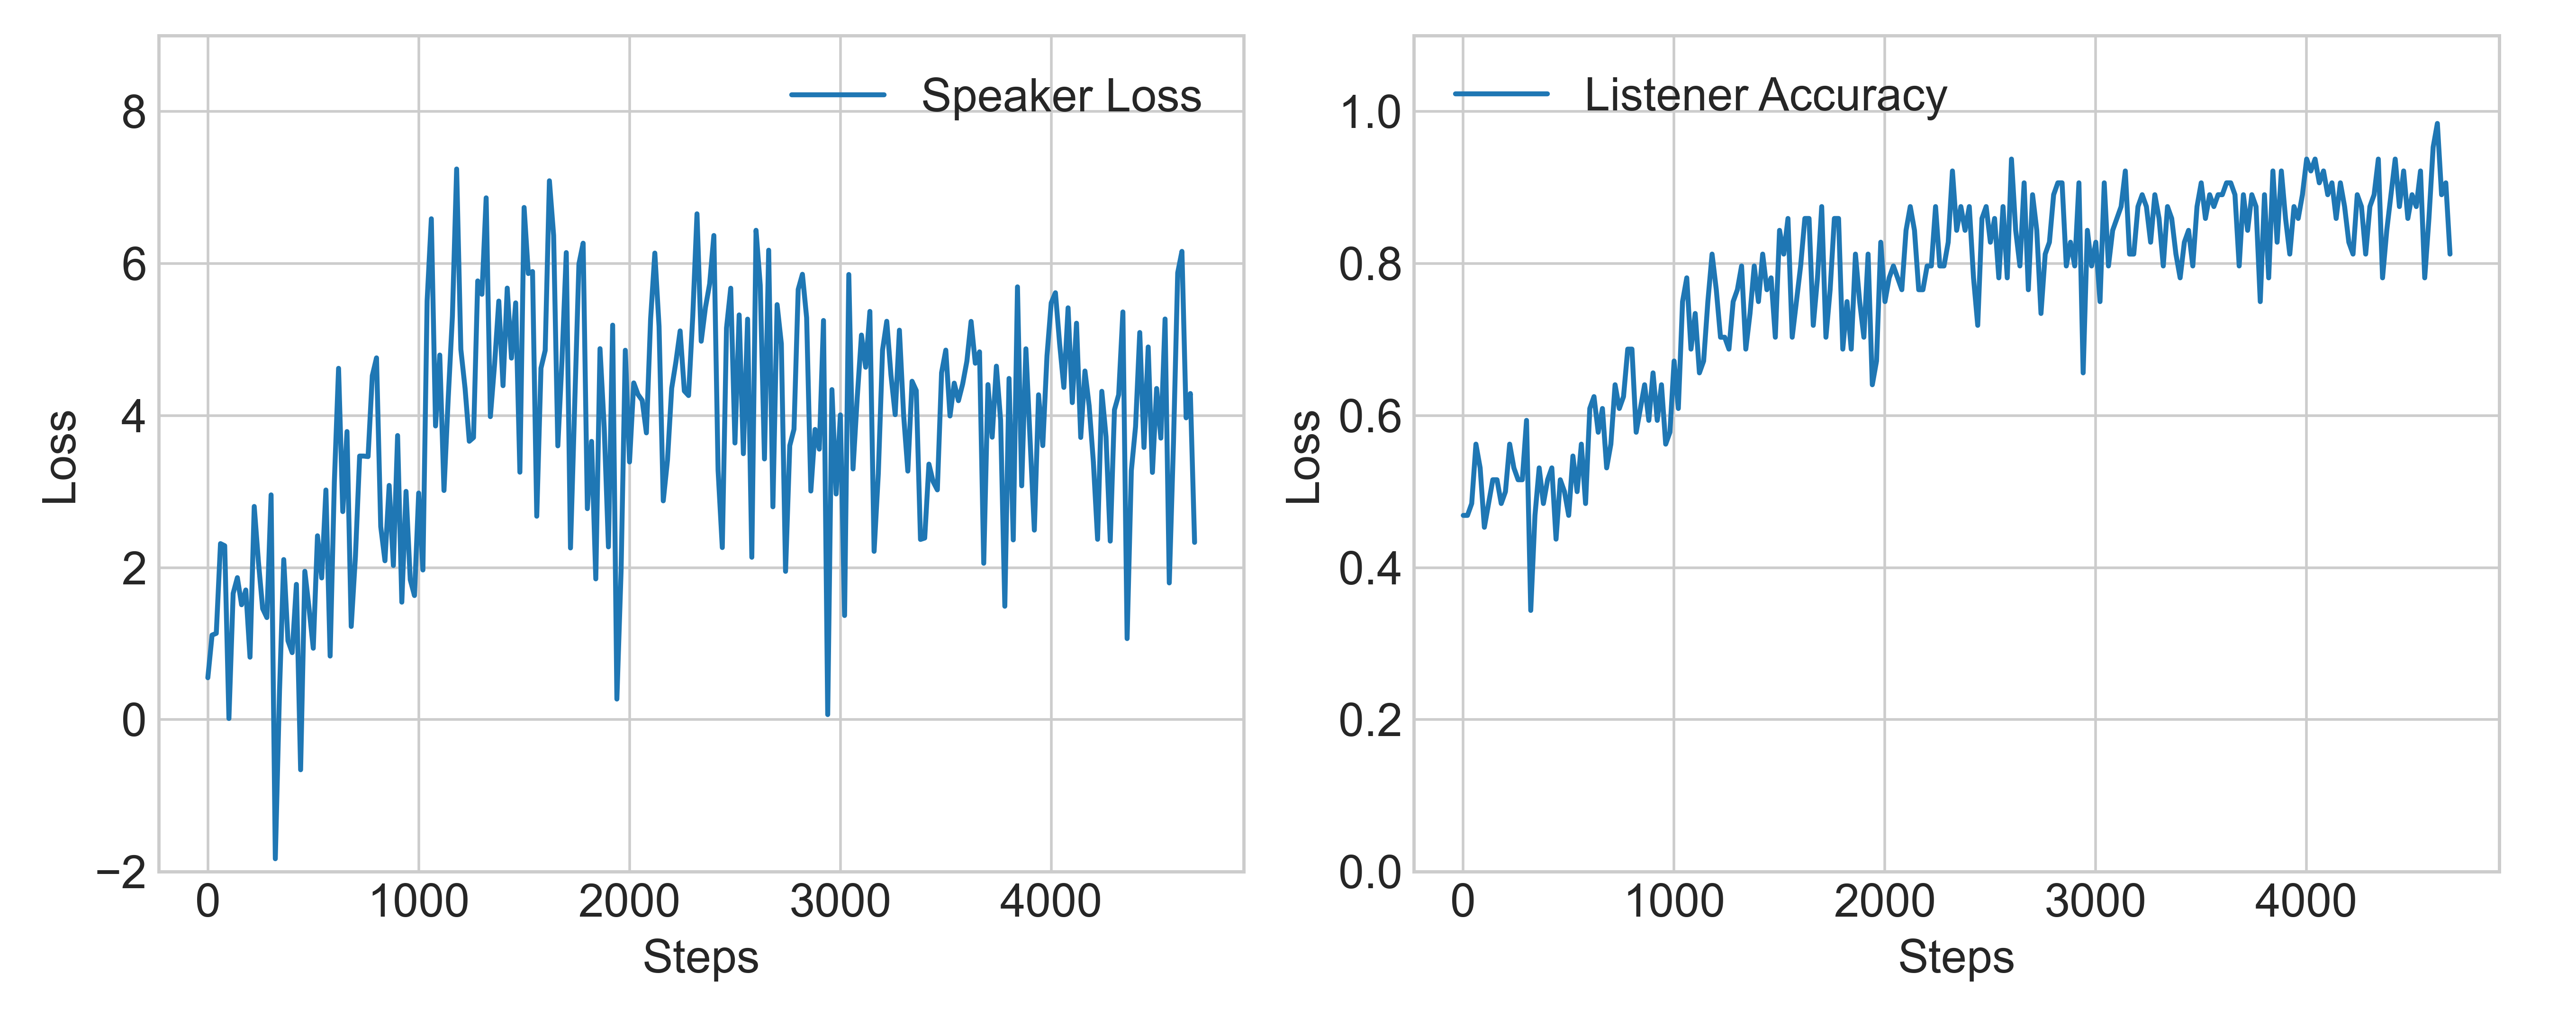
\includegraphics[width=\linewidth]{images/coco_refgame_4000_pure_075_random.png}
	\caption{Training results of the baseline MS COCO experiment (pure decoding, $\lambda_s = 0.75$). Left: Total speaker training loss. Right: Listener training accuracy.}
	\label{fig:coco_baseline_075_speaker_loss_listener_acc}
\end{figure}

\begin{figure}[h]
	\centering
	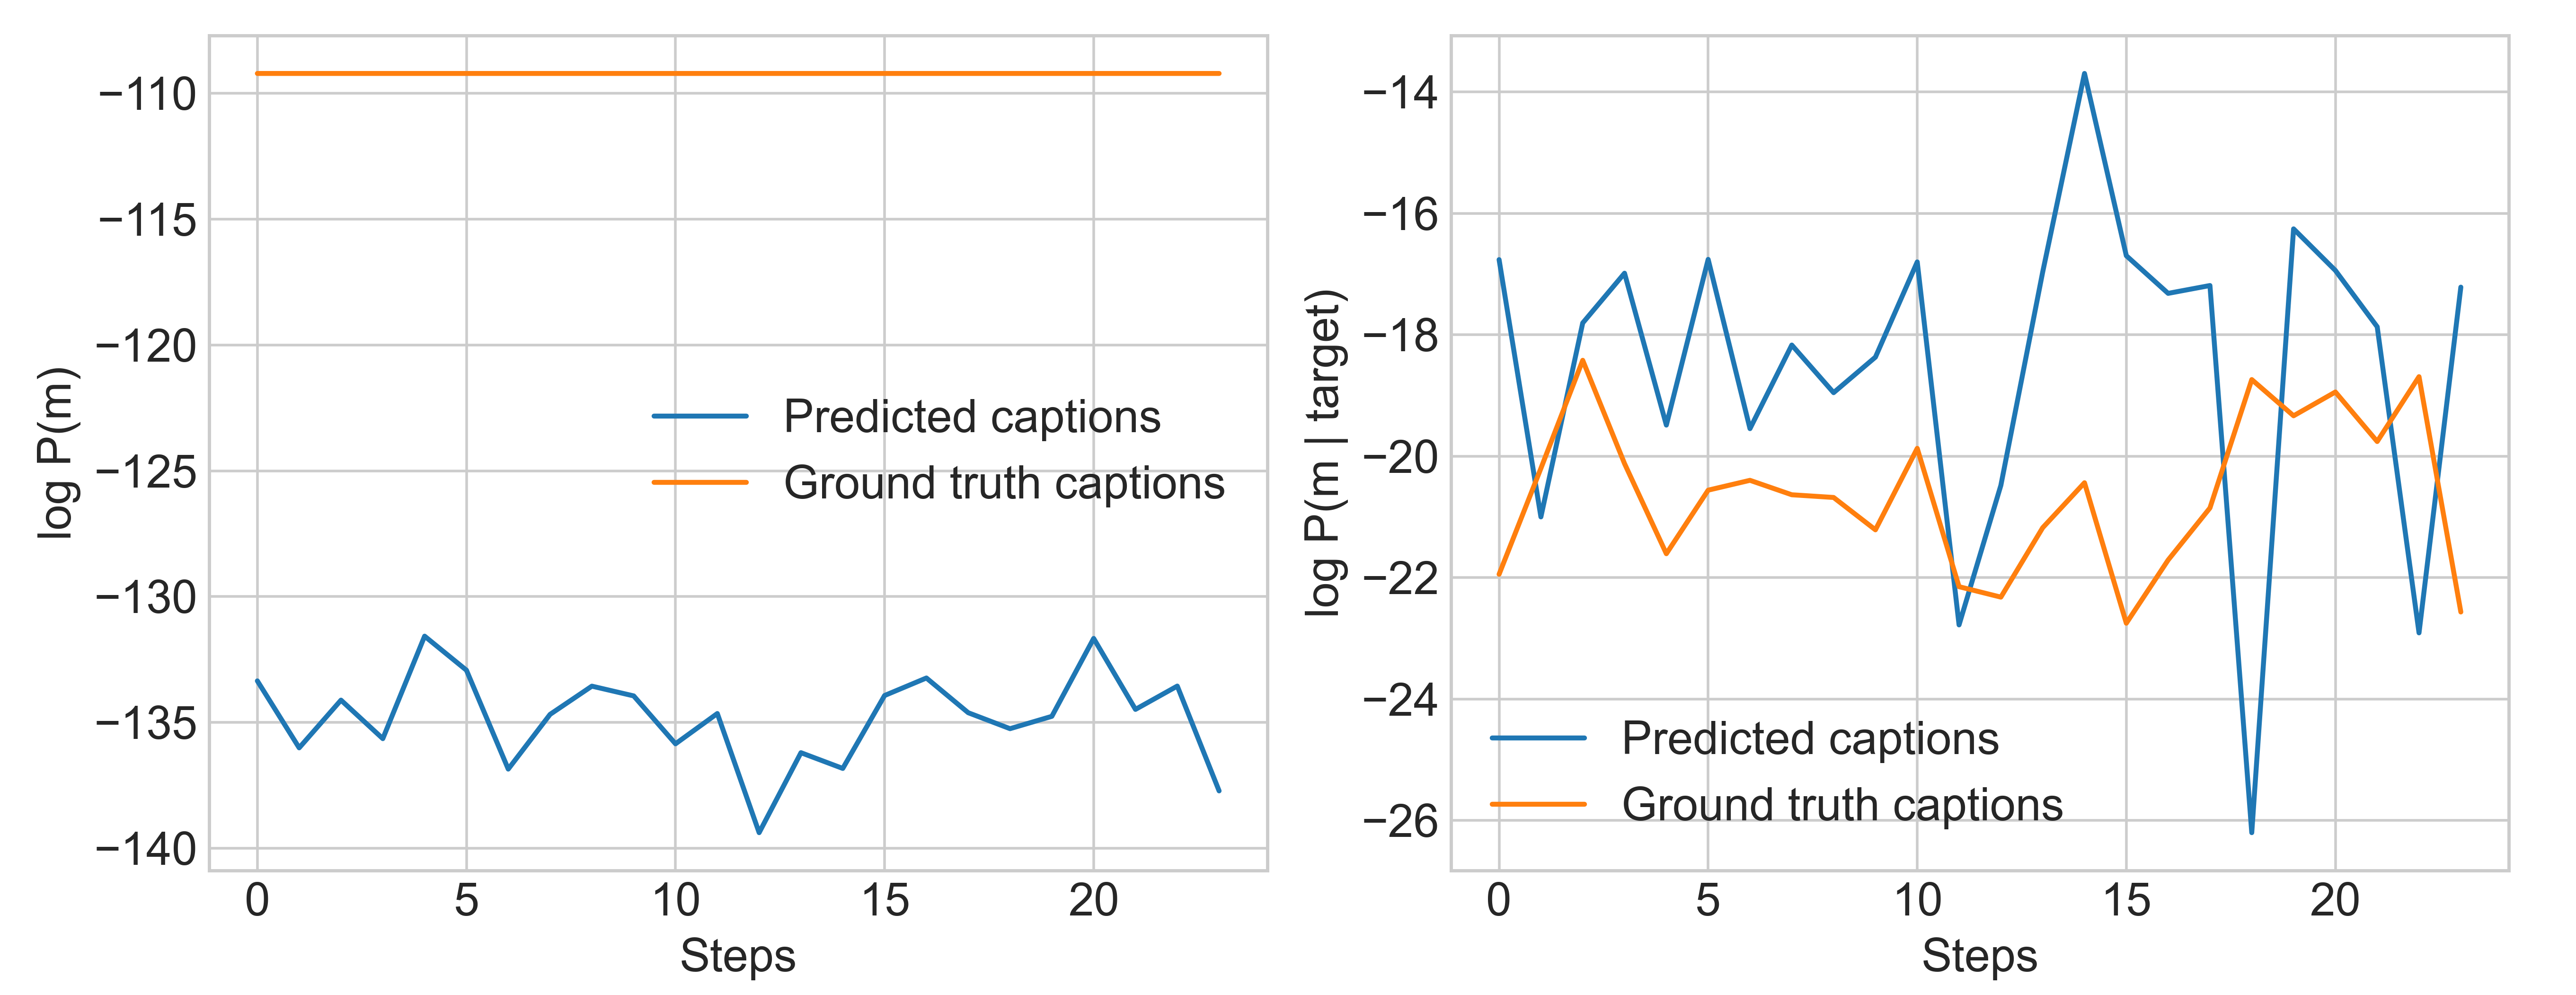
\includegraphics[width=\linewidth]{images/coco_structural_semantic_drift_4000_pure_075_random.png}
	\caption{Drift dynamics computed during training in the baseline MS COCO experiment (pure decoding, $\lambda_s = 0.75$). Higher values indicate less drift. Left: Structural drift of ground truth and predicted captions under the pretrained LM. Right: Semantic drift of ground truth and predicted captions under the pretrained speaker model.\protect\footnotemark}
	\label{fig:coco_baseline_075_str_drift}
\end{figure}
\footnotetext{Due to a coding error, semantic drifts were computed using greedy decoding on one image-caption pair only and, therefore, the values vary quite strongly.} 

For computing the test task accuracy, listener accuracy was computed on a held out validation set of 1000 pairs of images which were neither part of pretraining nor the reference game training. The test performance was estimated by sampling captions from the speaker using pure decoding, like during training, although it is also common to use greedy decoding at inference time in NLP. The test accuracy of 0.953 in Table \ref{tab:coco_drift_metrics_basic} shows that the agents successfully learned to play the reference game. Furthermore, supporting \textbf{H1} and \textbf{H2}, the language underwent deterioration, both syntactically and semantically, compared to the pretrained speaker. More specifically, the average log probability of the generated captions under the pretrained Transformer XL model decreased by 4.312, compated to the log probability of captions generated by the pretrained speaker. Similarly, the conditional log probability of the generated captions given the target images decreased by 9.434, compared to the conditional probability of the captions from the pretrained speaker (Table \ref{tab:coco_drift_metrics_basic}, first two columns, ``Pretrained MS speaker'' vs. ``MS Baseline, random, $\lambda_s=0.75$''). The dynamics of structural and semantic drifts during training can be seen in Figure \ref{fig:coco_baseline_075_str_drift}. To this end, following general procedure, the structural and semantic drift metrics were computed every 200 training steps on 192 held out image pairs (three batches). Due to the small size of the decrease as well as the small number of validation batches, no trend can be observed visually.\footnote{The number of metric computation steps was restricted to only three batches due to computational constraints.} 
As for the other drift metrics presented in Table \ref{tab:coco_drift_metrics_basic} (third and fourth columns), only anecdotal differences to the pretrained speaker can be observed: a slight increase in the discrete overlap metric might suggest that the speaker learned to produce messages that are more appropriate for the target compared to the distractor, and, therefore, might be more discriminative. On the other hand, the similarity of embeddings of the ground truth caption and the message decreased relative to the distractor similarity, compared to the pretrained speaker. This might be due to the difficulty to propagate the learning signal all the way to the embedding layer. Furthermore, the comparison to the overlap values of the ground truth captions indicates that the difference in terms of used tokens between target and distractor captions is much more pronounced in the dataset than what is propagated by the trained model (Tab.~\ref{tab:coco_drift_metrics_basic}, first line, third and fourth columns).  
Therefore, to sum up, \textbf{H3} is not borne out in this experiment.

\pt{Linear regressions will be computed on the drift values collected during the training.}

Additionally, the fine-tuned speaker was also evaluated with standard image captioning metrics. Table \ref{tab:eval_metrics_refgame} shows that caption quality marginally decreased with respect to almost all metrics, confirming the trend shown by the structural and semantic language drift metrics.

\subsubsection{Varying the structural loss weight}
In order to investigate \textbf{H4}, this experiment on MS COCO was also conducted with different structural loss weights $\lambda_s \in \{0, 0.25, 0.5, 1\}$. The training results (i.e., the speaker losses and listener accuracies during training) can be seen in Figure \ref{fig:coco_baseline_speaker_loss_listener_acc_all}. The main observation that can be made regarding the training dynamics is that the magnitude of the loss strongly depends on the weight of the structural loss $\lambda_s$---the smaller the weight, the larger are the total loss values (Fig.~\ref{fig:coco_baseline_speaker_loss_listener_acc_all}, left). This can be attributed to the larger weight of the functional loss, respectively, which is computed with REINFORCE and might be subject to stronger variance \parencite[cf.][]{havrylov2017emergence}. However, varying the weight did not have visible effects on the listener's ability to learn the reference game (Fig.~\ref{fig:coco_baseline_speaker_loss_listener_acc_all}, right). 
This is supported by the comparably high test listener accuracy values in Table \ref{tab:coco_drift_metrics_basic} (fifth column). If anything, against general intuitions from the literature, the task performance is slightly worse with higher functional pressure (test accuracy of 0.924 with functional loss only), compared to higher structural pressure (test accuracy of 0.953 with $\lambda_s = 0.75$). But consistent with intuition, the accuracy in the experiment where the speaker was trained with structural pressure only ($\lambda_s = 1$), the listener accuracy is almost identical to the accuracy computed against the pretrained speaker. This confirms that training the speaker with the structural loss only amounts to further training the pretrained model, which was already pretrained to convergence (see Fig.~\ref{fig:coco_pretraining}) and, therefore, did not improve much.

%This could indicate that the listener is flexible enough to adapt to the speaker's messages, essentially independently of their nature. This hints at speaker-listener co-adaptation. 
\begin{figure}[h]
	\centering
	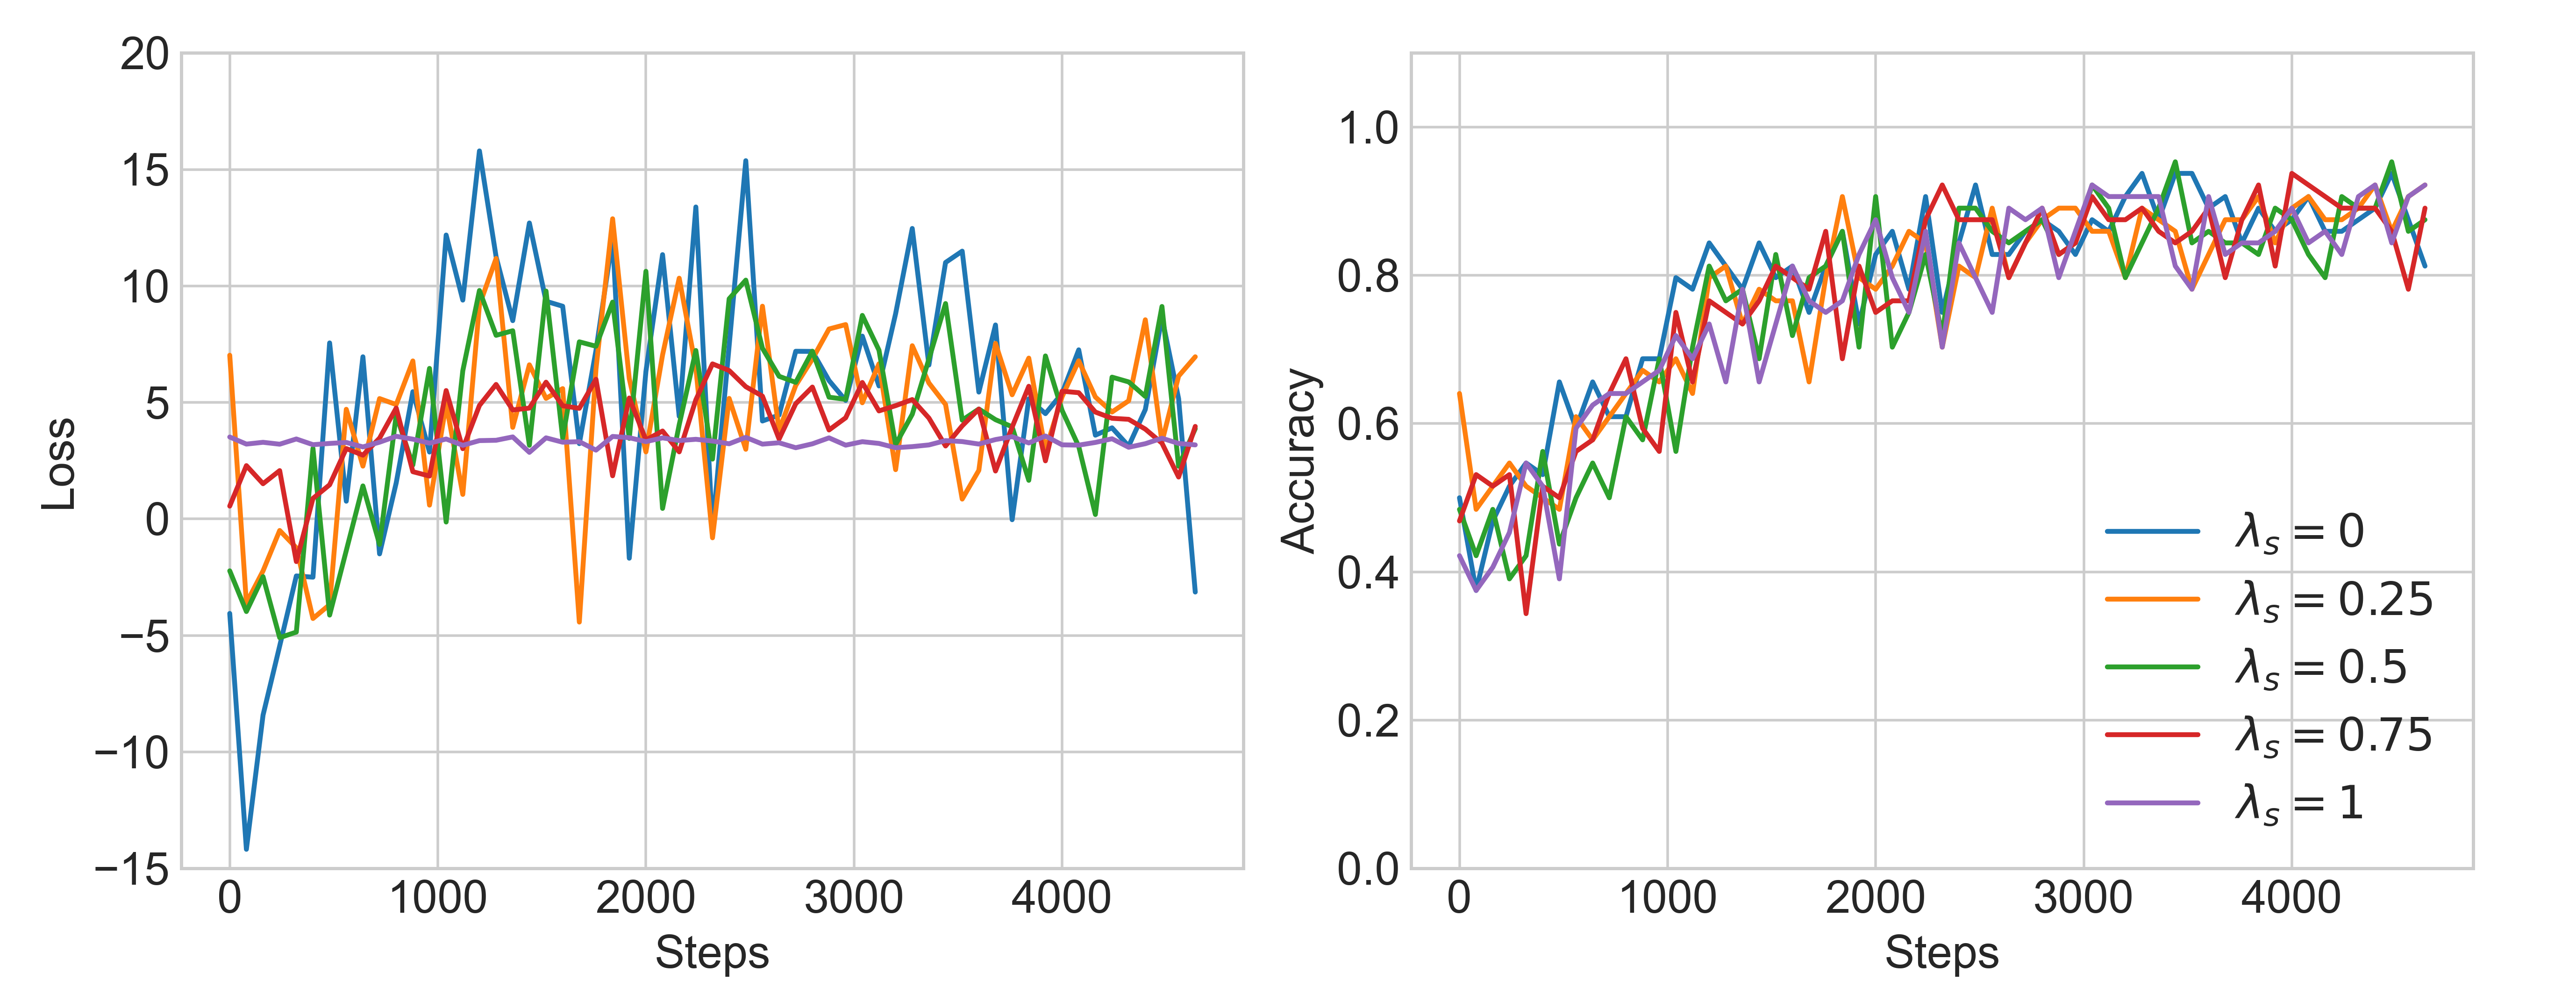
\includegraphics[width=\linewidth]{images/coco_refgame_4000_pure_all_Ls_random.png}
	\caption{Training results of the MS COCO experiment with varying $\lambda_s$ (pure decoding, random pairs). Left: Total speaker training loss. Right: Listener training accuracy.}
	\label{fig:coco_baseline_speaker_loss_listener_acc_all}
\end{figure}

Table \ref{tab:coco_drift_metrics_basic} also provides a comparison of the drift metrics for the different loss configurations. Based on naive comparison, if anything, the structural and semantic drifts were smaller when the structural pressure on the speaker was \emph{smaller}, contrary to a priori intuition. That is, when the pressure to stay close to the initially learned image captioning language distribution was smaller, the produced messages had a higher likelihood both under the pretrained LM and the pretrained speaker. The absence of a clear difference between the drift results is also supported by the drift dynamics computed during training (see Fig. \ref{fig:coco_baseline_str_sem_drift_all}). 
The drift values for the experiment with $\lambda_s = 0$ also speak against \textbf{H1} and \textbf{H2}. Somewhat surprisingly, semantic drift values were lower for the generated captions compared to the ground truth captions (Fig.~\ref{fig:coco_baseline_str_sem_drift_all}), indicating that the generated captions were generally more likely given the target image, than the ground truth captions, under the pretrained speaker model. This could be attributed to the auto-regressive pretraining of the speaker, which might have resulted in generally better performance in the auto-regressive generation mode, compared to ground truth availability (see Appendix \ref{app:grid_search} and Section \ref{architecture}).
\begin{figure}
	\centering
	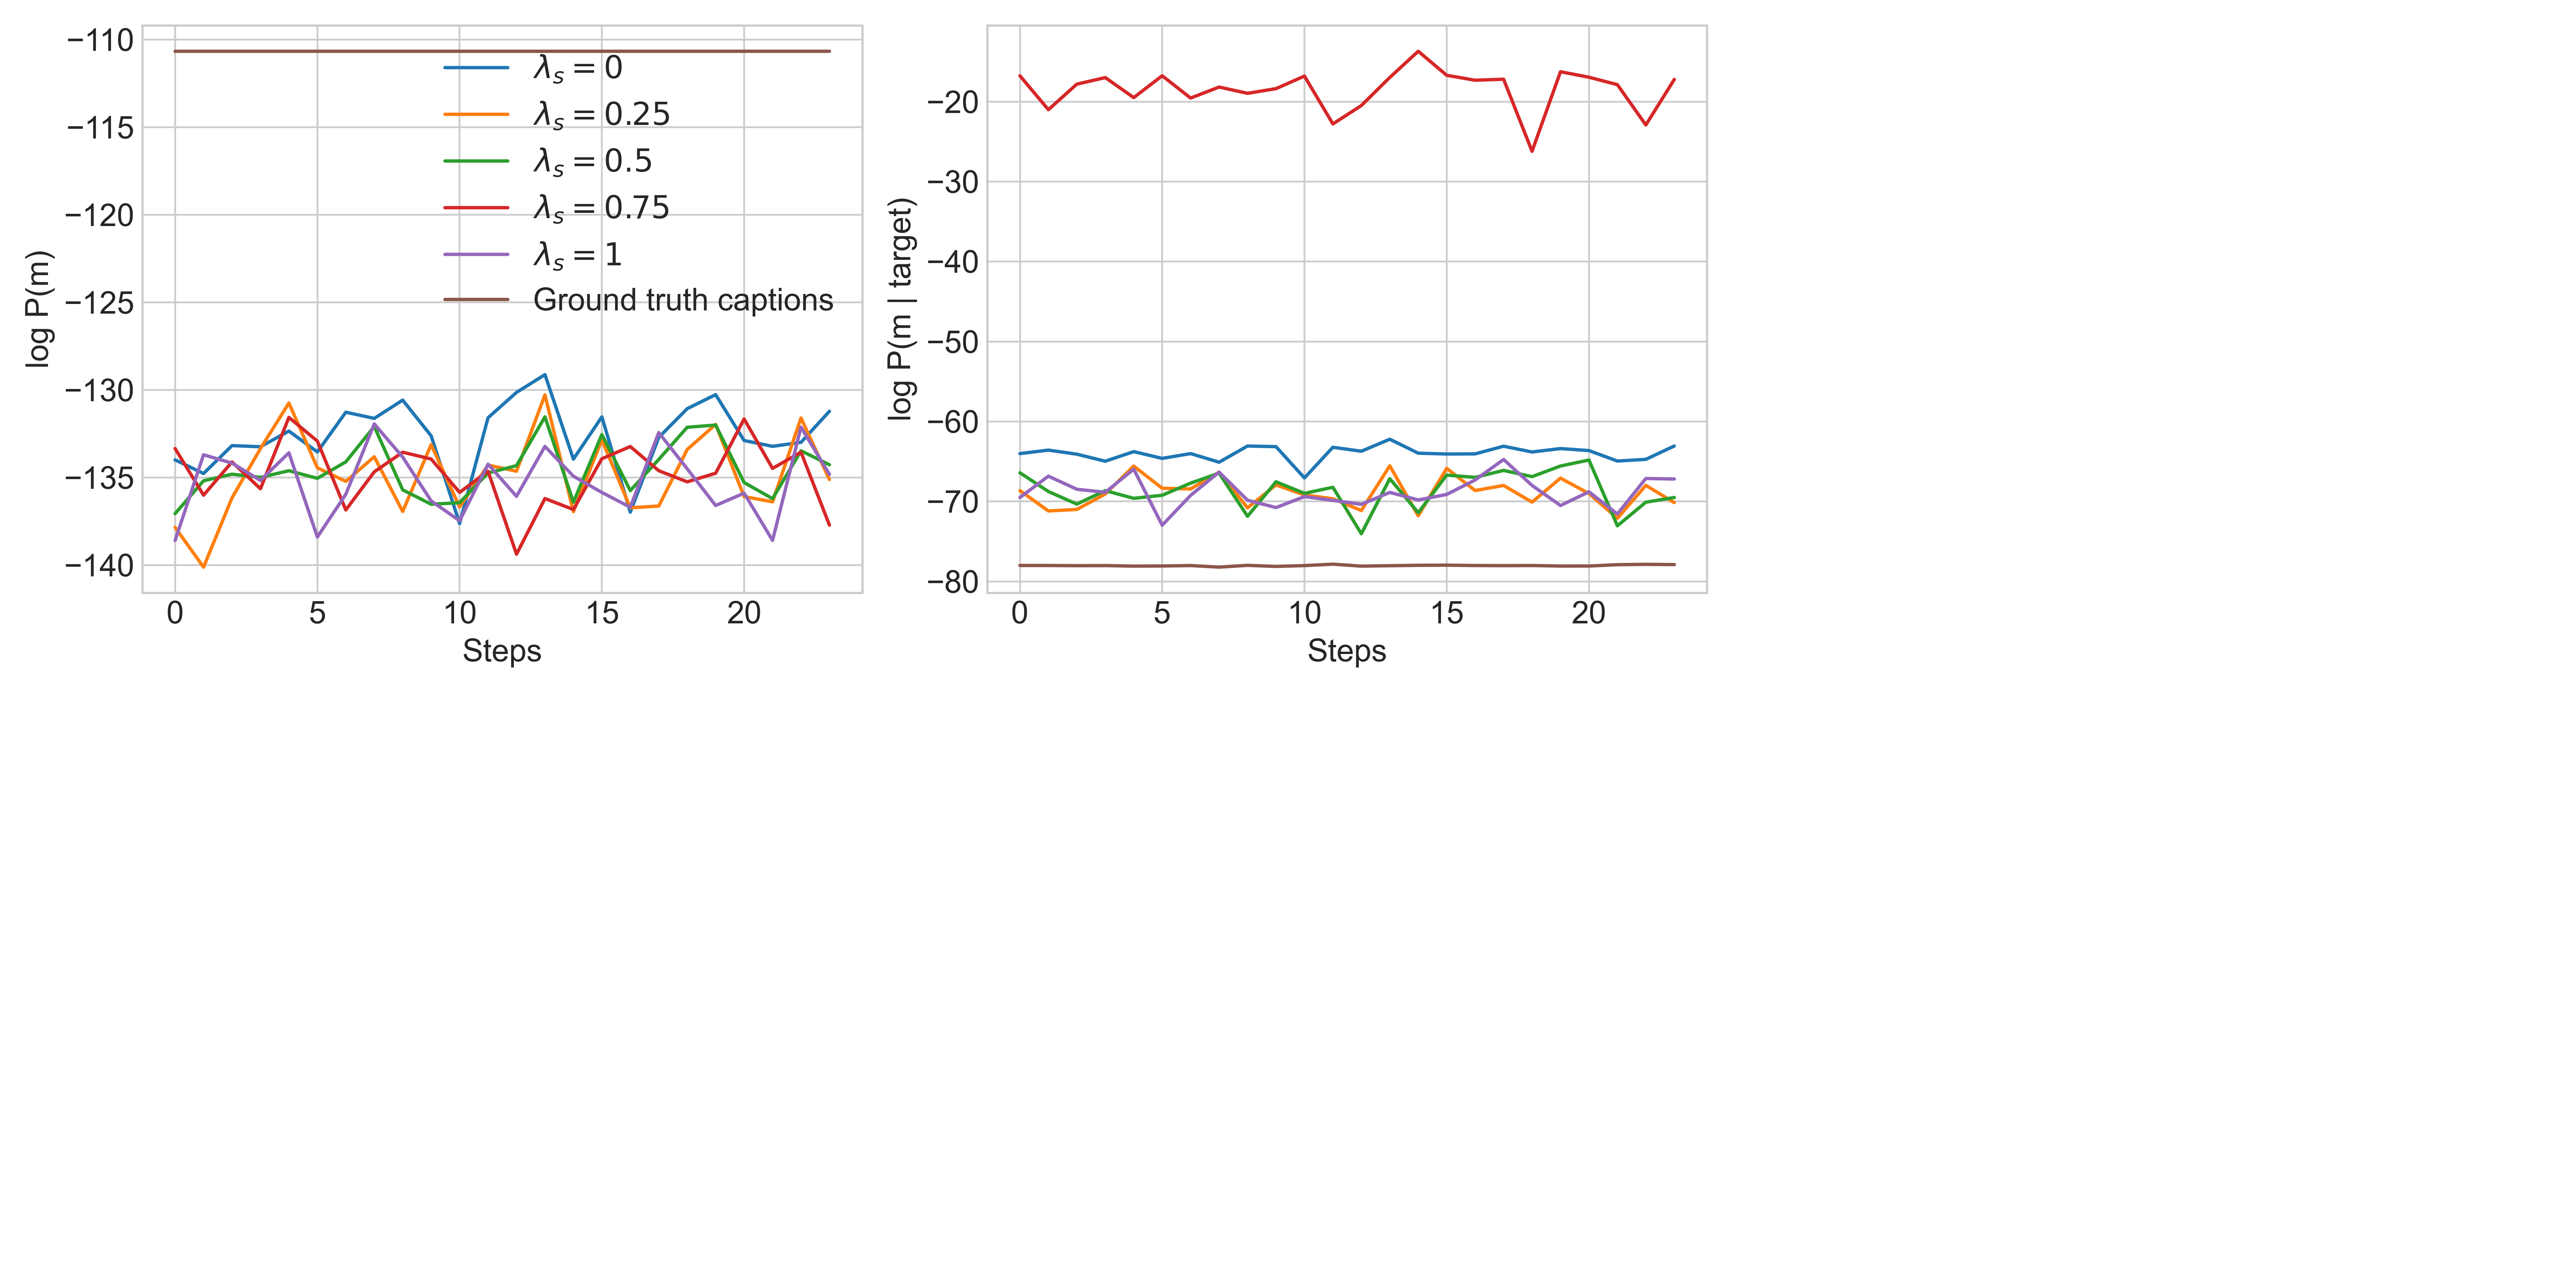
\includegraphics[width=\linewidth]{images/coco_structural_semantic_drift_4000_pure_L_S_all_random.png}
	\caption{Drift dynamics computed during training in the baseline MS COCO experiments (pure decoding) with varying $\lambda_s$ weights. Left: Structural drift of ground truth and predicted captions under the pretrained LM. Right: Semantic drift of ground truth and predicted captions under the pretrained speaker model. Due to a coding error, the semantic drift of the $\lambda_s = 0.75$ model is represented as the mean validation conditional log probability from Tab.~\ref{tab:coco_drift_metrics_basic}.}
	\label{fig:coco_baseline_str_sem_drift_all}
\end{figure}

One reason for the structural drift results might be that the model trained with \emph{less} structural pressure produced messages that were more likely under a pretrained language model. As noted above, the pretrained speaker produced messages that were not very well-formed on a surface level \pt{as can be seen from these examples, ADD}, most likely due to the involvement of the auto-regressive pretraining mode (see Appendix \ref{app:grid_search}). Therefore, it might be expected that a speaker which was more strongly forced to stay close to the pretraining language distribution produced less structurally well-formed sentences, under a pretrained LM. The more functionally oriented speaker, on the other hand, might by chance produce better sentences, even if the respective learning signal is not related to the LM. Lastly, it could be hypothesized that these drift results are rather snapshots of the speaker's performance, especially for the speakers with lower $\lambda_s$, since their policies did not converge after training the agents for only two training epochs, as can be seen from the respective loss plot (Fig. \ref{fig:coco_baseline_speaker_loss_listener_acc_all}, left). 
Turning towards the other drift metrics in Table \ref{tab:coco_drift_metrics_basic}, again, there is no indication of a clear trend in connection to the structural loss weight. Nevertheless, the discrete overlap has the highest value for the $\lambda_s = 0$ experiment (0.065 higher than for the pretrained speaker), indicating that the strong functional pressure on the speaker might have led to generating captions capturing more of the target image's properties.

The speakers trained with the different loss configurations were also evaluated using image captioning metrics; the results are reported in Table \ref{tab:eval_metrics_refgame}. Generally, they also follow the trends indicated by the drift metrics, although the differences in values are marginal.

To sum up, given the presented training configurations, \textbf{H4} is not supported by the results. However, based on the grid search over speaker configurations conducted prior to the main experiments (see the difference in reference game performances in Appendix \ref{app:grid_search}, Fig.~\ref{fig:coco_grid_Ls_decoding_TF_only}), one might hypothesize that the presence of effects of the structural loss weight is connected to the presence of auto-regressive pretraining of the speaker agent. That is, it could be critical that the speaker is already pretrained with the caption generation mode, as it then plays a role for the structural loss computation in the reference game. Follow-up experiments regarding this effect of pretraining mode would fill a gap in extant literature \parencite[but see][for related work]{lowe2020interaction}.

\subsection{MS COCO: Similar Pairs Experiments}
\label{expt:coco_similar_pairs}
In order to investigate \textbf{H5}, an experiment with similar image pairs was conducted. That is, the goal was to increase the similarity of target and distractor images and thereby increase the pressure to produce more specific messages in reference to the target \parencite[cf.][]{graf2016animal}. As described in Section \ref{ds:coco}, the pairs were constructed by picking the ones depicting at least three identical basic-level categories, as provided by the dataset annotations. Therefore, arguably the similarity of the images was conceptual, which also likely implied a certain degree of perceptual similarity. In order to validate experimental results, similar to the random pairs experiments, the agents' task performance and language drift were tested on 1000 held out \emph{similar} image pairs. 
Otherwise, the training configurations matched the baseline experiment. 

\begin{figure}[h]
	\centering
	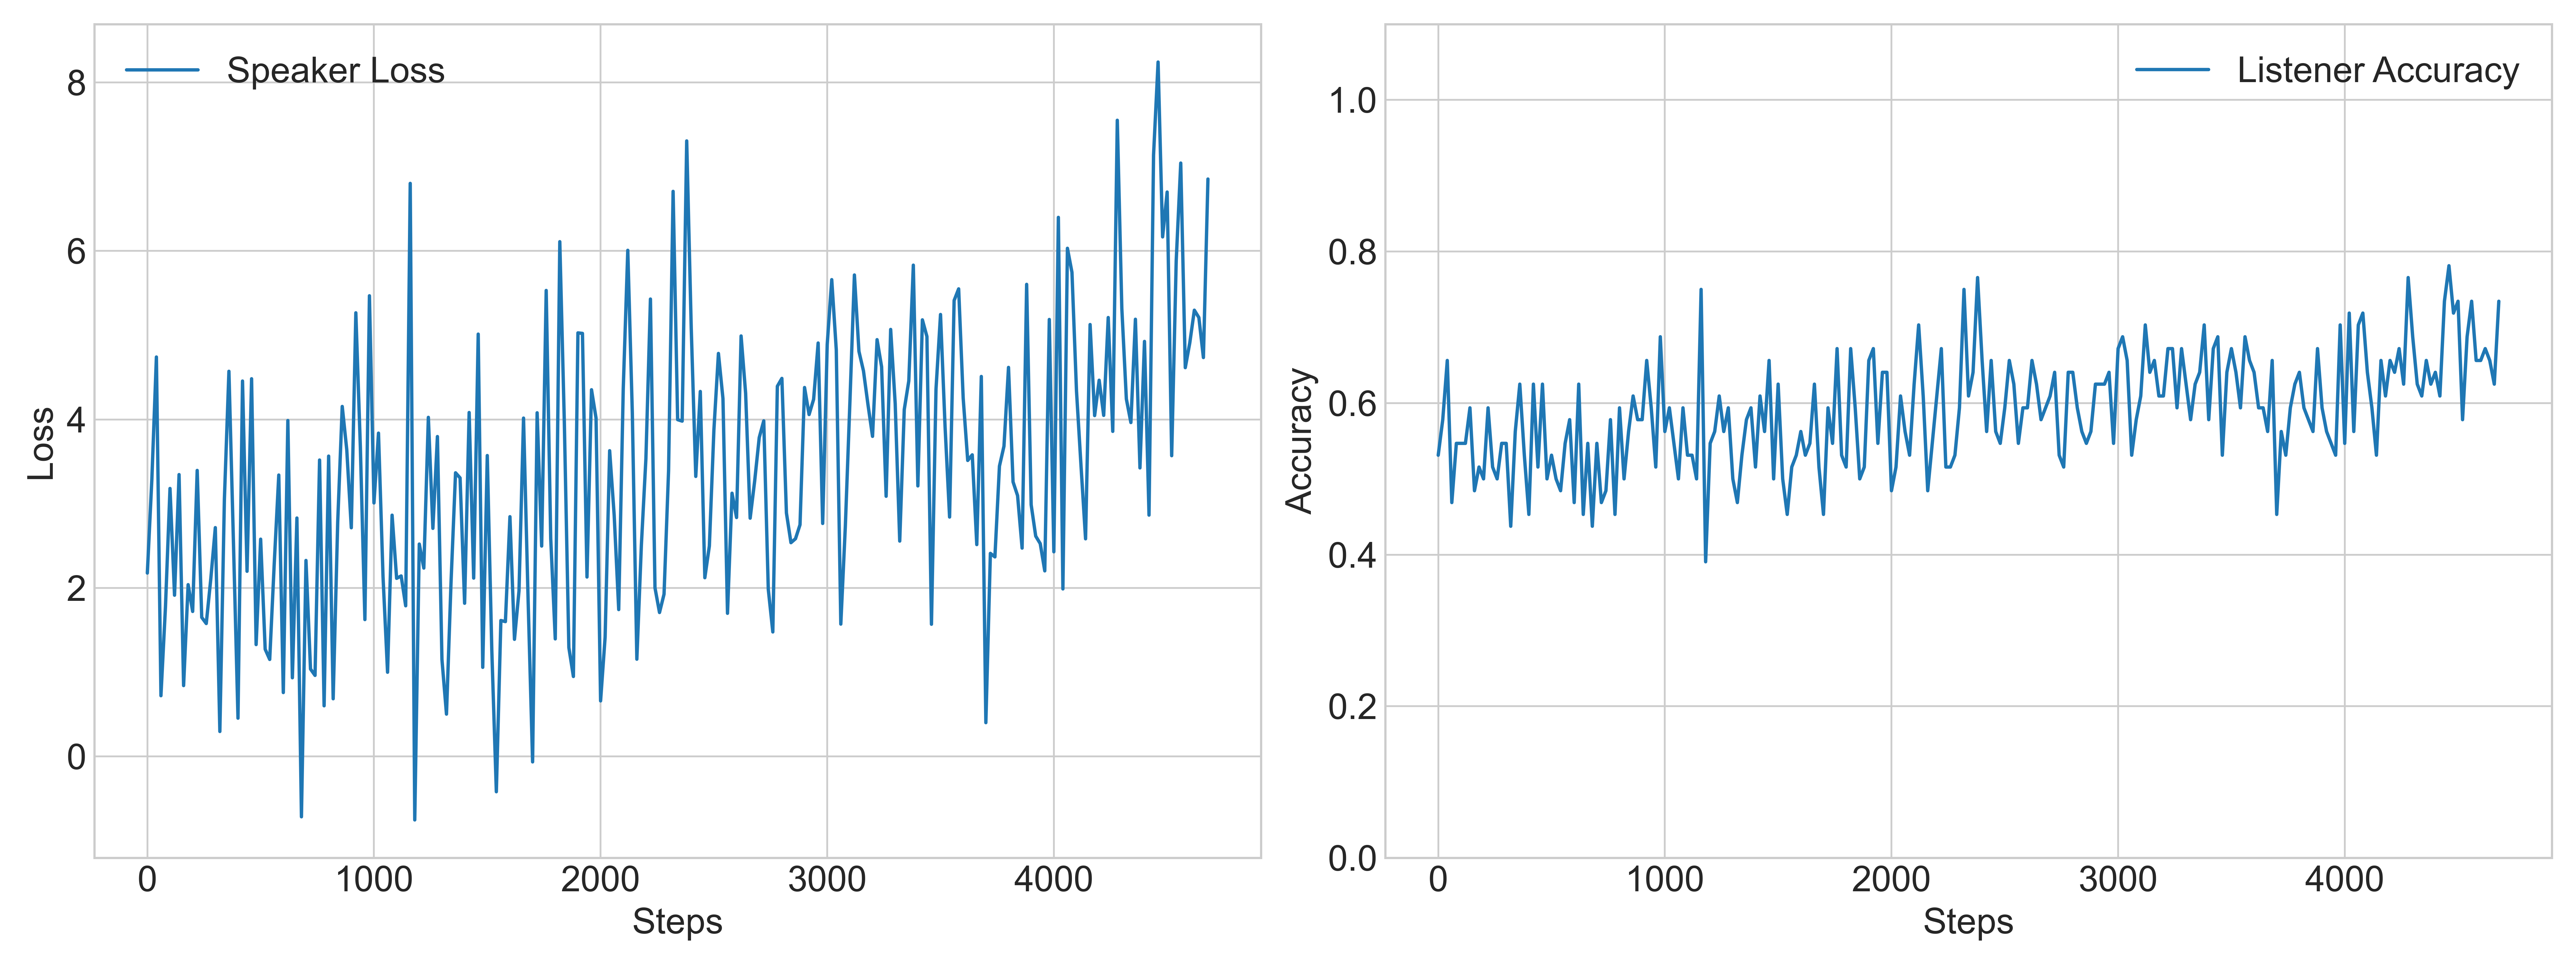
\includegraphics[width=\linewidth]{images/coco_similarFixed_075_losses.png}
	\caption{Training results of the MS COCO experiment with similar target-distractor image pairs ($\lambda_s=0.75$, pure decoding). Left: Total speaker training loss. Right: Listener training accuracy.}
	\label{fig:coco_similar_speaker_loss_listener_acc_all}
\end{figure}

\begin{figure}[h]
	\centering
	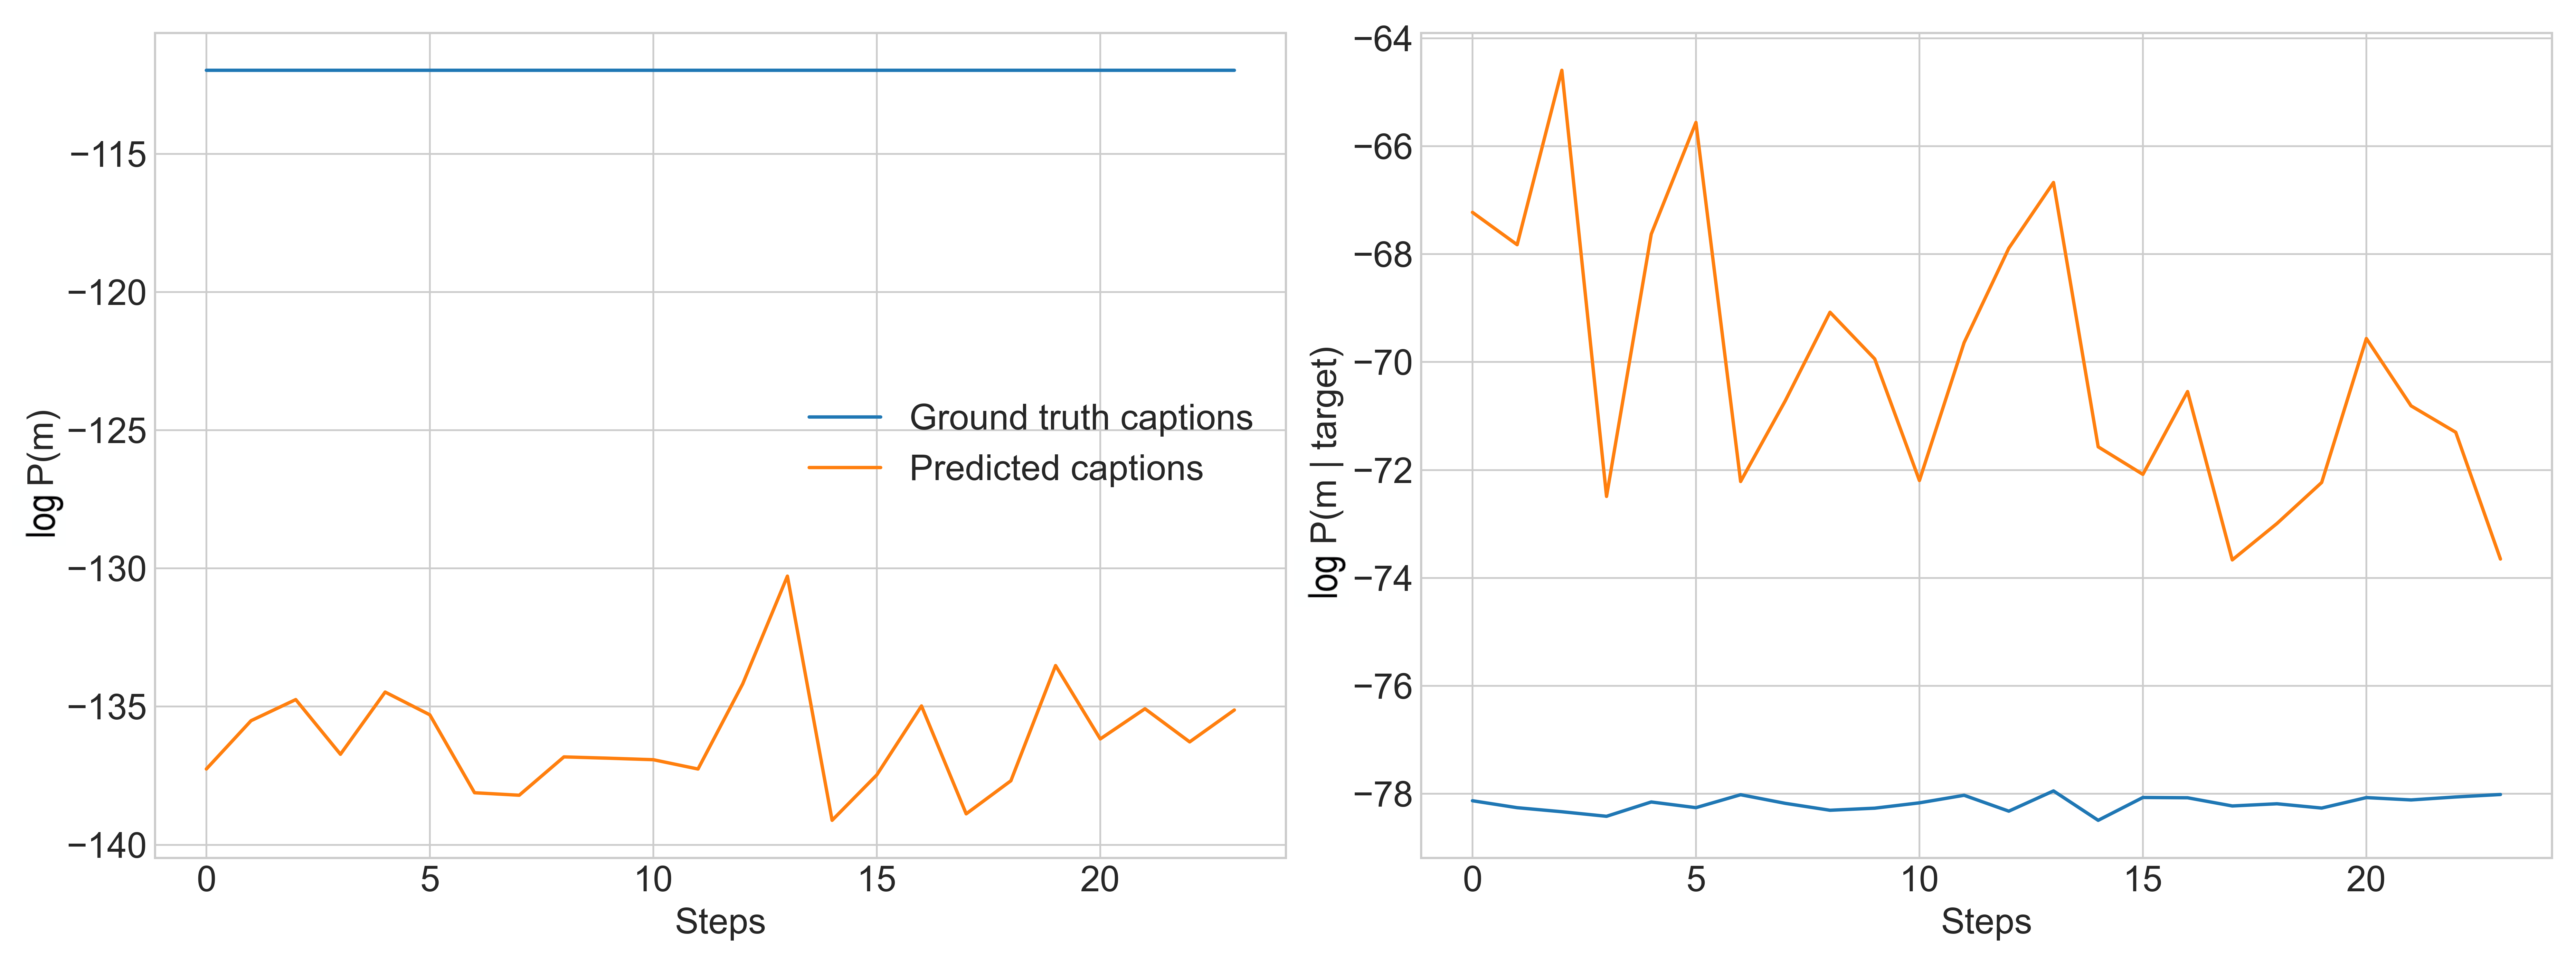
\includegraphics[width=\linewidth]{images/coco_structural_semantic_drift_4000_pure_075_similarFixed.png}
	\caption{Drift dynamics computed during training on similar target-distractor image pairs on MS COCO experiments (pure decoding, $\lambda_s=0.75$). Left: Structural drift of ground truth and predicted captions under the pretrained LM. Right: Semantic drift of ground truth and predicted captions under the pretrained speaker model.}
	\label{fig:coco_similar_str_sem_drift_all}
\end{figure}

Figure \ref{fig:coco_similar_speaker_loss_listener_acc_all} shows the training dynamics of this experiment; compared to the baseline experiment (Fig.~\ref{fig:coco_baseline_075_speaker_loss_listener_acc}), it is clear that it was much more difficult for the agents to learn the reference game. In fact, visually, they only started improving on the task towards the end of the two training epochs, suggesting that they should be trained longer. This difficulty to learn the task can be attributed to the difficulty of grounding the listener in perceptually similar images with messages which are likely applicable to both images to some extent, making the functional training signal rather weak. This is confirmed by a low listener test accuracy of 0.648, compared to random pairs experiments (Tab.~\ref{tab:coco_drift_metrics_basic}). This confirms the agents' sensitivity to the context in which the target occurs. 

This difficulty of grounding the listener led to increasing speaker-listener co-adaptation during training, compared to baseline experiments, as shown by the increasing semantic drift (Fig.~\ref{fig:coco_similar_str_sem_drift_all}, right). This means that instead of learning the `ground truth' meaning of the speaker's words, the listener and the speaker built new conventions, more effective for this similar input. No such trend is visible for structural drift (Fig.~\ref{fig:coco_similar_str_sem_drift_all}, left); its dynamics are comparable to the baseline experiments (Fig.~\ref{fig:coco_baseline_str_sem_drift_all}, left). 
However, both structural and semantic language drift on the test set were lower for the similar pairs than for the random pairs experiments, indicating that it is the strength of the functional signal that was likely responsible for both structural and semantic drift. That is, since it was more difficult for the listener to learn the task and, therefore, the task-based feedback to the speaker was less conclusive than for random pairs, the speaker did not adapt her messages as strongly.
At the same time, the decrease in discrete overlap indicates that it was more difficult for the speaker to find words that are true of the target but not the distractor. On the other hand, the decrease might also indicate that the speaker might have learned to mention more novel features of the target which were not part of the ground truth caption, compared to random pairs experiments and the pretrained speaker. Following the idea behind this value as a functional drift metric, it decreased with decreasing task success, compared to the random pairs experiment value. No clear difference in continuous overlap compared to random experiments was observed.

\begin{figure}[h]
	\centering
	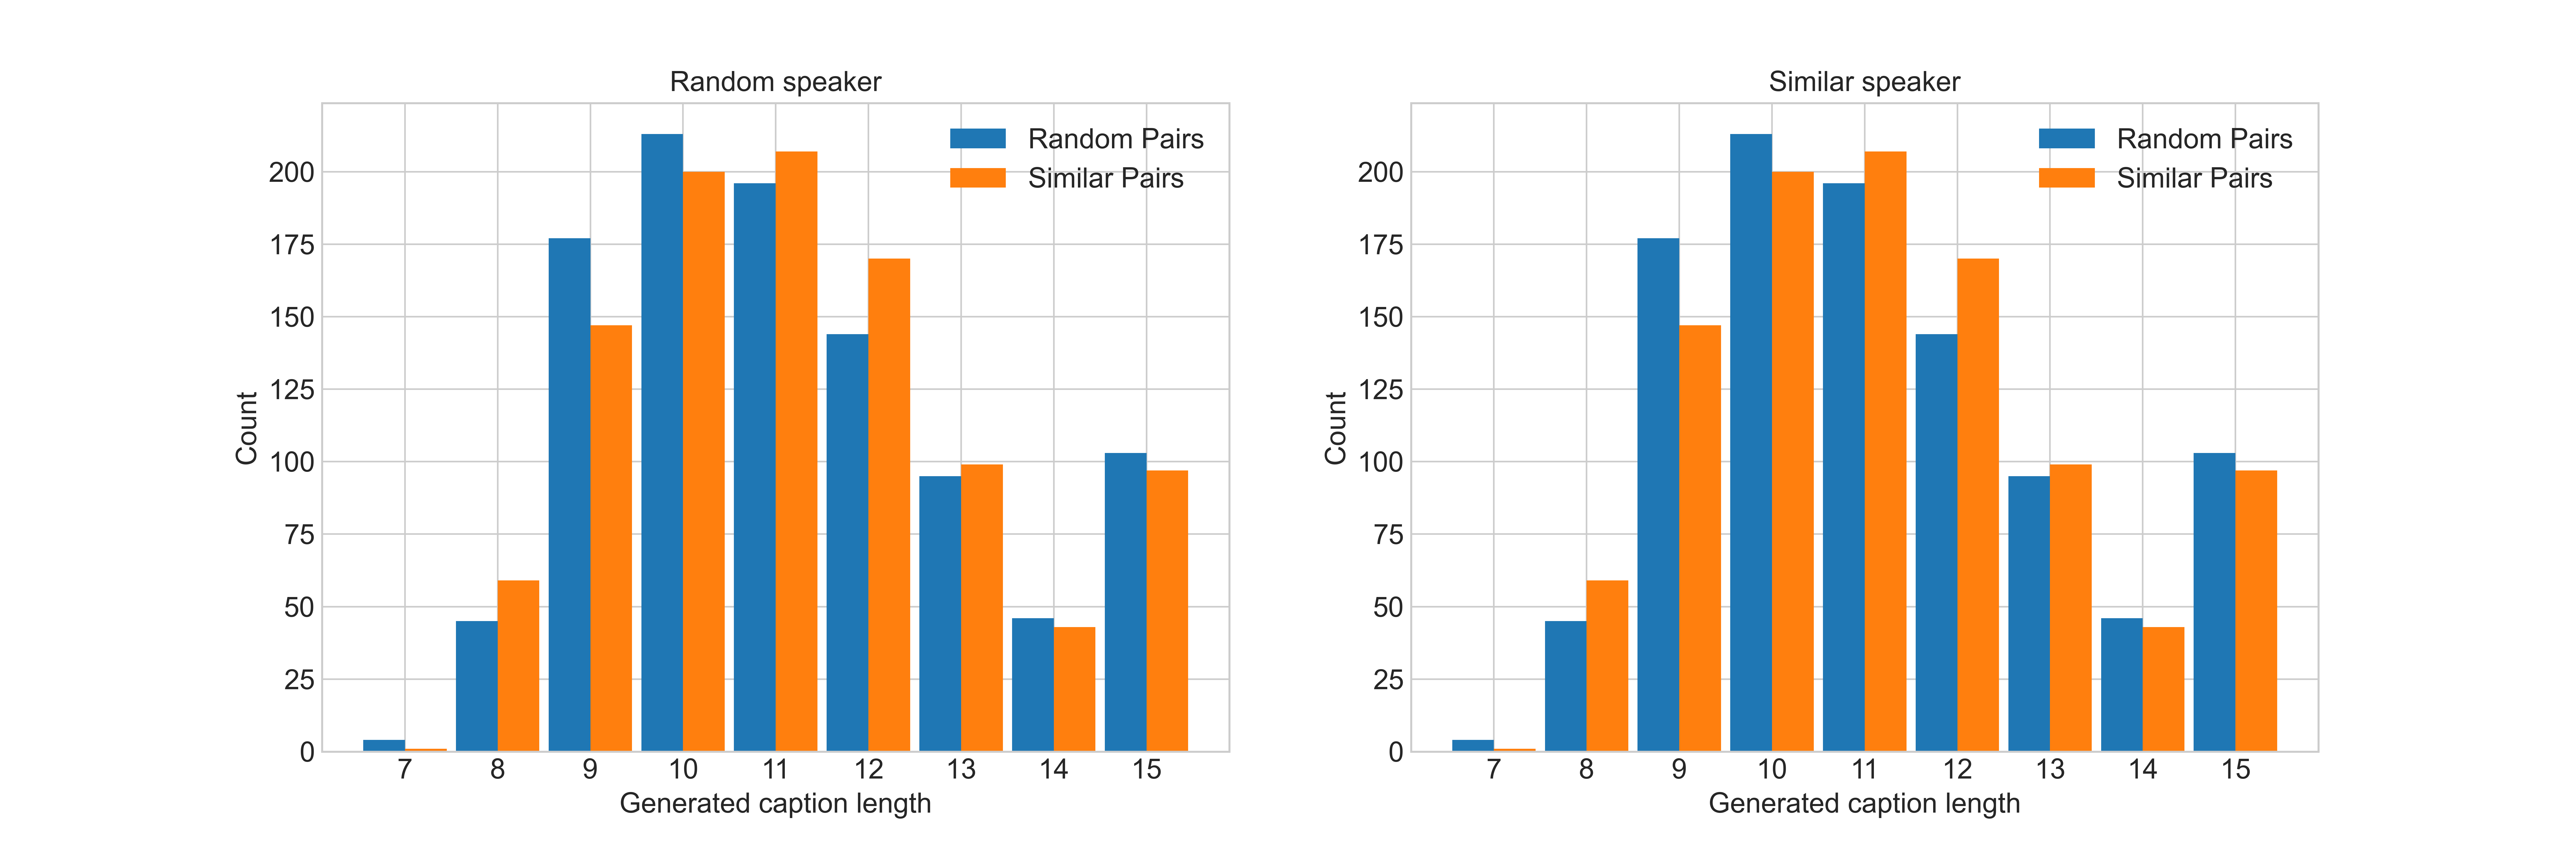
\includegraphics[width=\linewidth]{images/coco_random_similar_length_counts.png}
	\caption{Distribution of produced sentences' lengths given similar and random target-distractor image pairs. Left: Speaker trained on the baseline random pairs reference game. Right: Speaker trained on the similar pairs reference game.}
	\label{fig:coco_similar_random_speaker_lengths}
\end{figure}
In order to investigate the second part of \textbf{H5}, namely whether the specificity of the speaker's messages in the similar pairs experiment increased, the lengths of the messages generated on the test set were investigated. To this end, the number of tokens until the first special END token was computed (excluding it). The lengths of messages generated by the speaker from the baseline experiment (Section \ref{expt:coco_baseline}) was compared to those of the speaker from this experiment, given similar test image pairs versus random test image pairs (Fig.~\ref{fig:coco_similar_random_speaker_lengths}). The figure shows a slight trend towards longer messages for similar images pairs, suggesting that, supporting the hypothesis, the speaker used more words in order to refer to more difficult targets. However, it also suggests that this was the case for both speakers, i.e., that this tendency did not emerge due to exposure to similar training pairs in this experiment compared to the random baseline, but rather might be the result of speaker pretraining (cf.~Section~\ref{speaker_pretraining}). Because they were pretrained on pairs of images, it might be the case that the speakers implicitly learned to put the target in context of the distractor, and, therefore, produced this trend.
\begin{figure}[h]
	\centering
	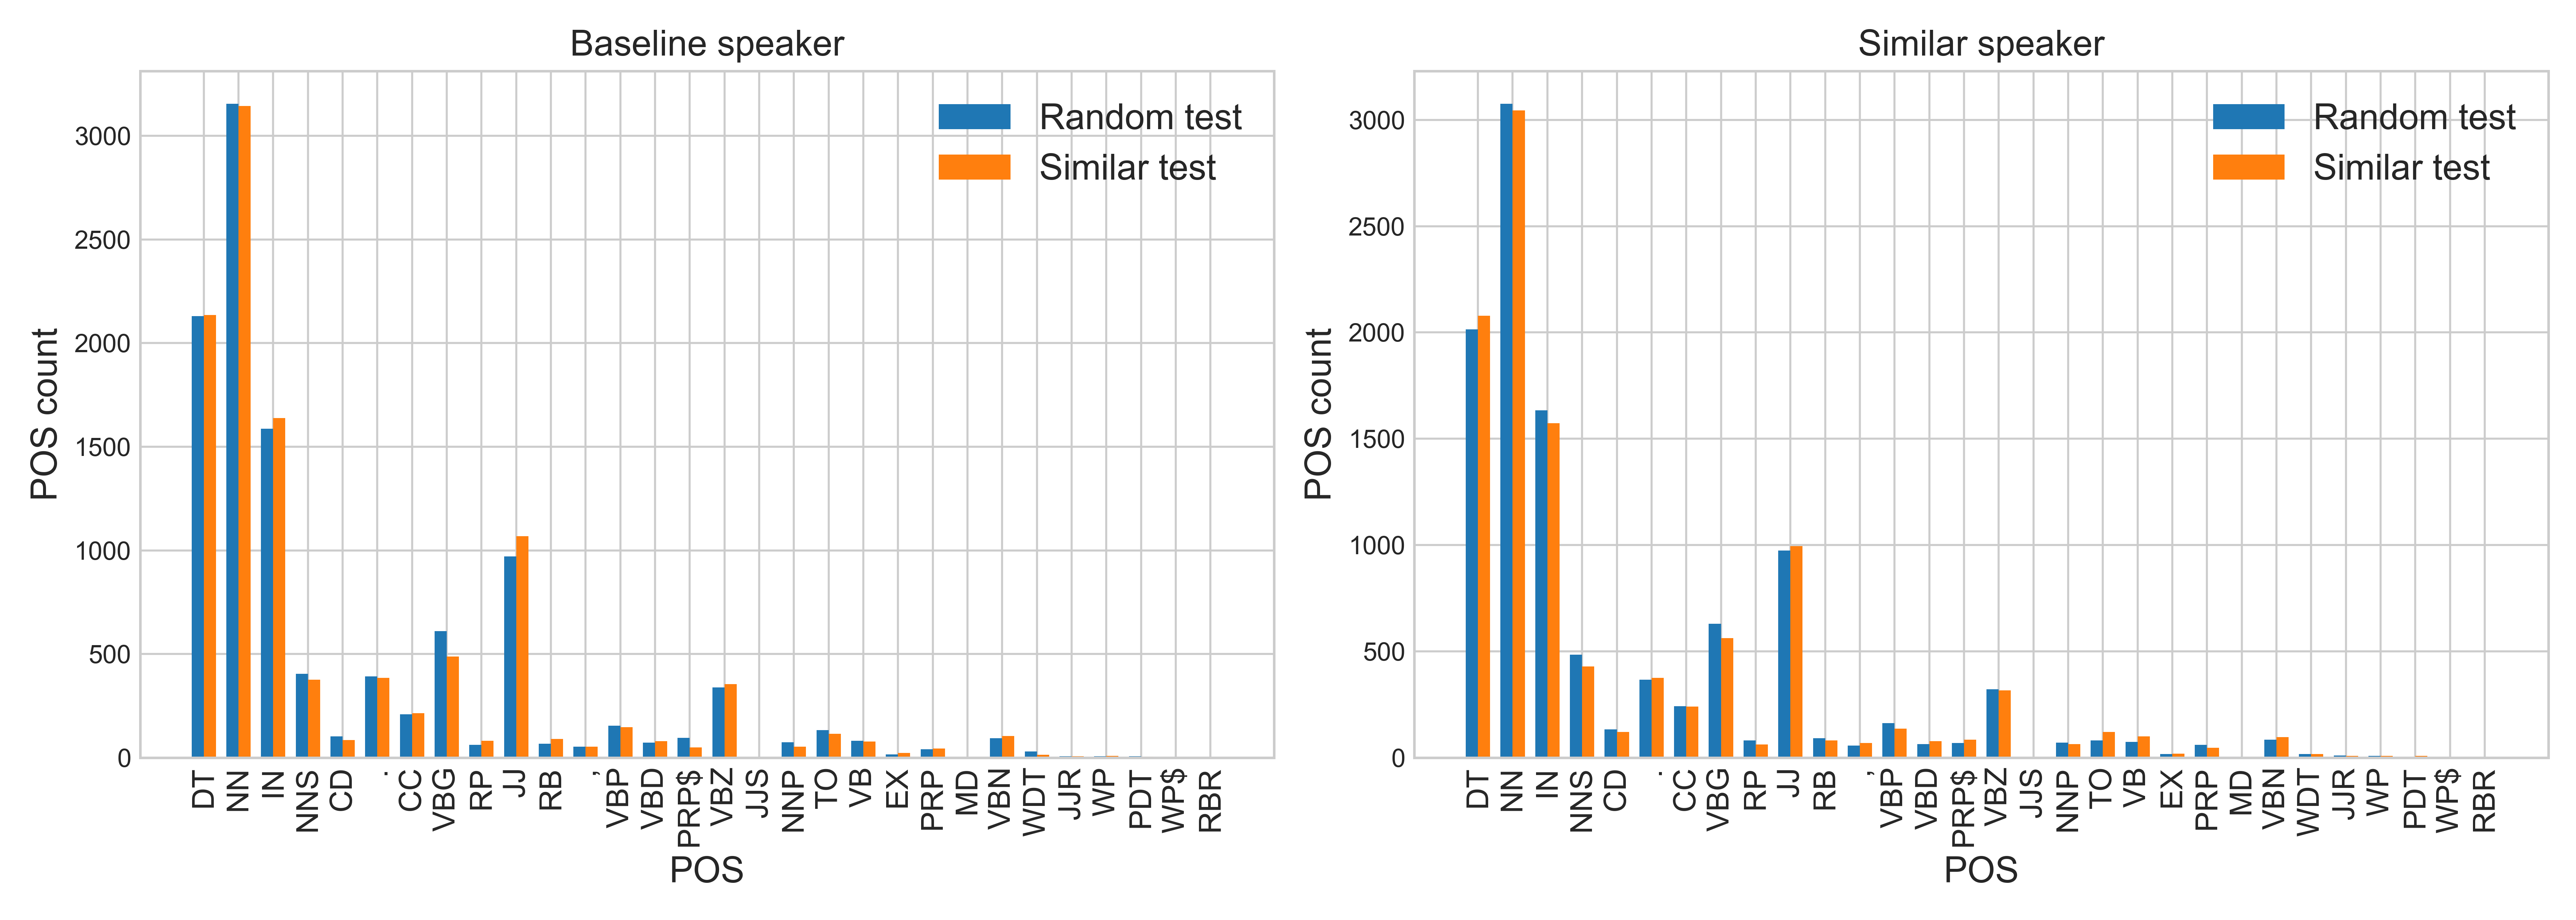
\includegraphics[width=\linewidth]{images/coco_similar_v_baseline_randomTest_vs_similarTest_POS_counts.png}
	\caption{Distribution of POS tags in produced sentences lengths given similar and random target-distractor image pairs. Left: Speaker trained on the baseline random pairs reference game. Right: Speaker trained on the similar pairs reference game.}
	\label{fig:coco_similar_random_speaker_POS}
\end{figure}
To further zoom in on the granularity of the productions, the produced messages were tagged with parts of speech (POS) tags with the \texttt{nltk} package \parencite{bird2006nltk} and the distribution of the tags was compared for the baseline and this experiment. Figure \ref{fig:coco_similar_random_speaker_POS} shows that the were small differences in the parts of speech preferred for either type of image pairs, but no decisive trends or differences between the baseline speaker and the speaker from the similar pairs experiment are visible. This also indicates that differences may potentially rather stem from the pretrained speaker's sensitivity towards the distractor. Additionally, taken together, these analyses indicate that the speaker of the similar pairs experiment did not learn particular strategies of referring to the target, compared to random image pairs, which most likely may be due to the complexity of the task and the short reference game training time.

To sum up, these results support \textbf{H5} in that the speaker's messages are less discriminative given more similar target-distractor pairs. They do not provide conclusive evidence that the speaker produced more granular messages for similar image pairs. They nonetheless confirm that the agents are highly sensitive to the visual context of their task.

\subsection{MS COCO: Fixed Listener Experiments}
\label{exp:coco_fixed_listener}
In order to investigate \textbf{H6}, a reference game with random pairs and $\lambda_s=0.75$ was conducted with a \emph{fixed} listener. That, is the speaker was fine-tuned to produce discriminative captions while being provided the task success signal by an already pretrained listener which was not further trained during the reference game, as opposed to receiving the task success signal from a \emph{joint} listener which learns to complete the task and ground the speaker's messages during the reference game. To this end, the listener was pretrained for four epochs to optimally interpret ground truth image captions. The same images as for the speaker pretraining were used. That is, the listener agent saw random pairs of images and received the ground truth caption for the target and was optimized to identify the target. After pretraining, the fixed listener's test accuracy on the ground truth captions of a held out dataset of 1000 images was 0.963. The test accuracy on messages generated by the pretrained speaker for the same images was 0.902.

The goal of this experiment was to investigate language drift in absence of speaker-listener co-adaptation which arises when the two agents are trained together. By having a fixed pretrained listener, intuitively, the speaker cannot improve the message discriminativity by finding `loopholes' and establishing specific conventions with the listener, and should be forced to use the ground truth grounding of the messages.

\begin{figure}
	\centering
	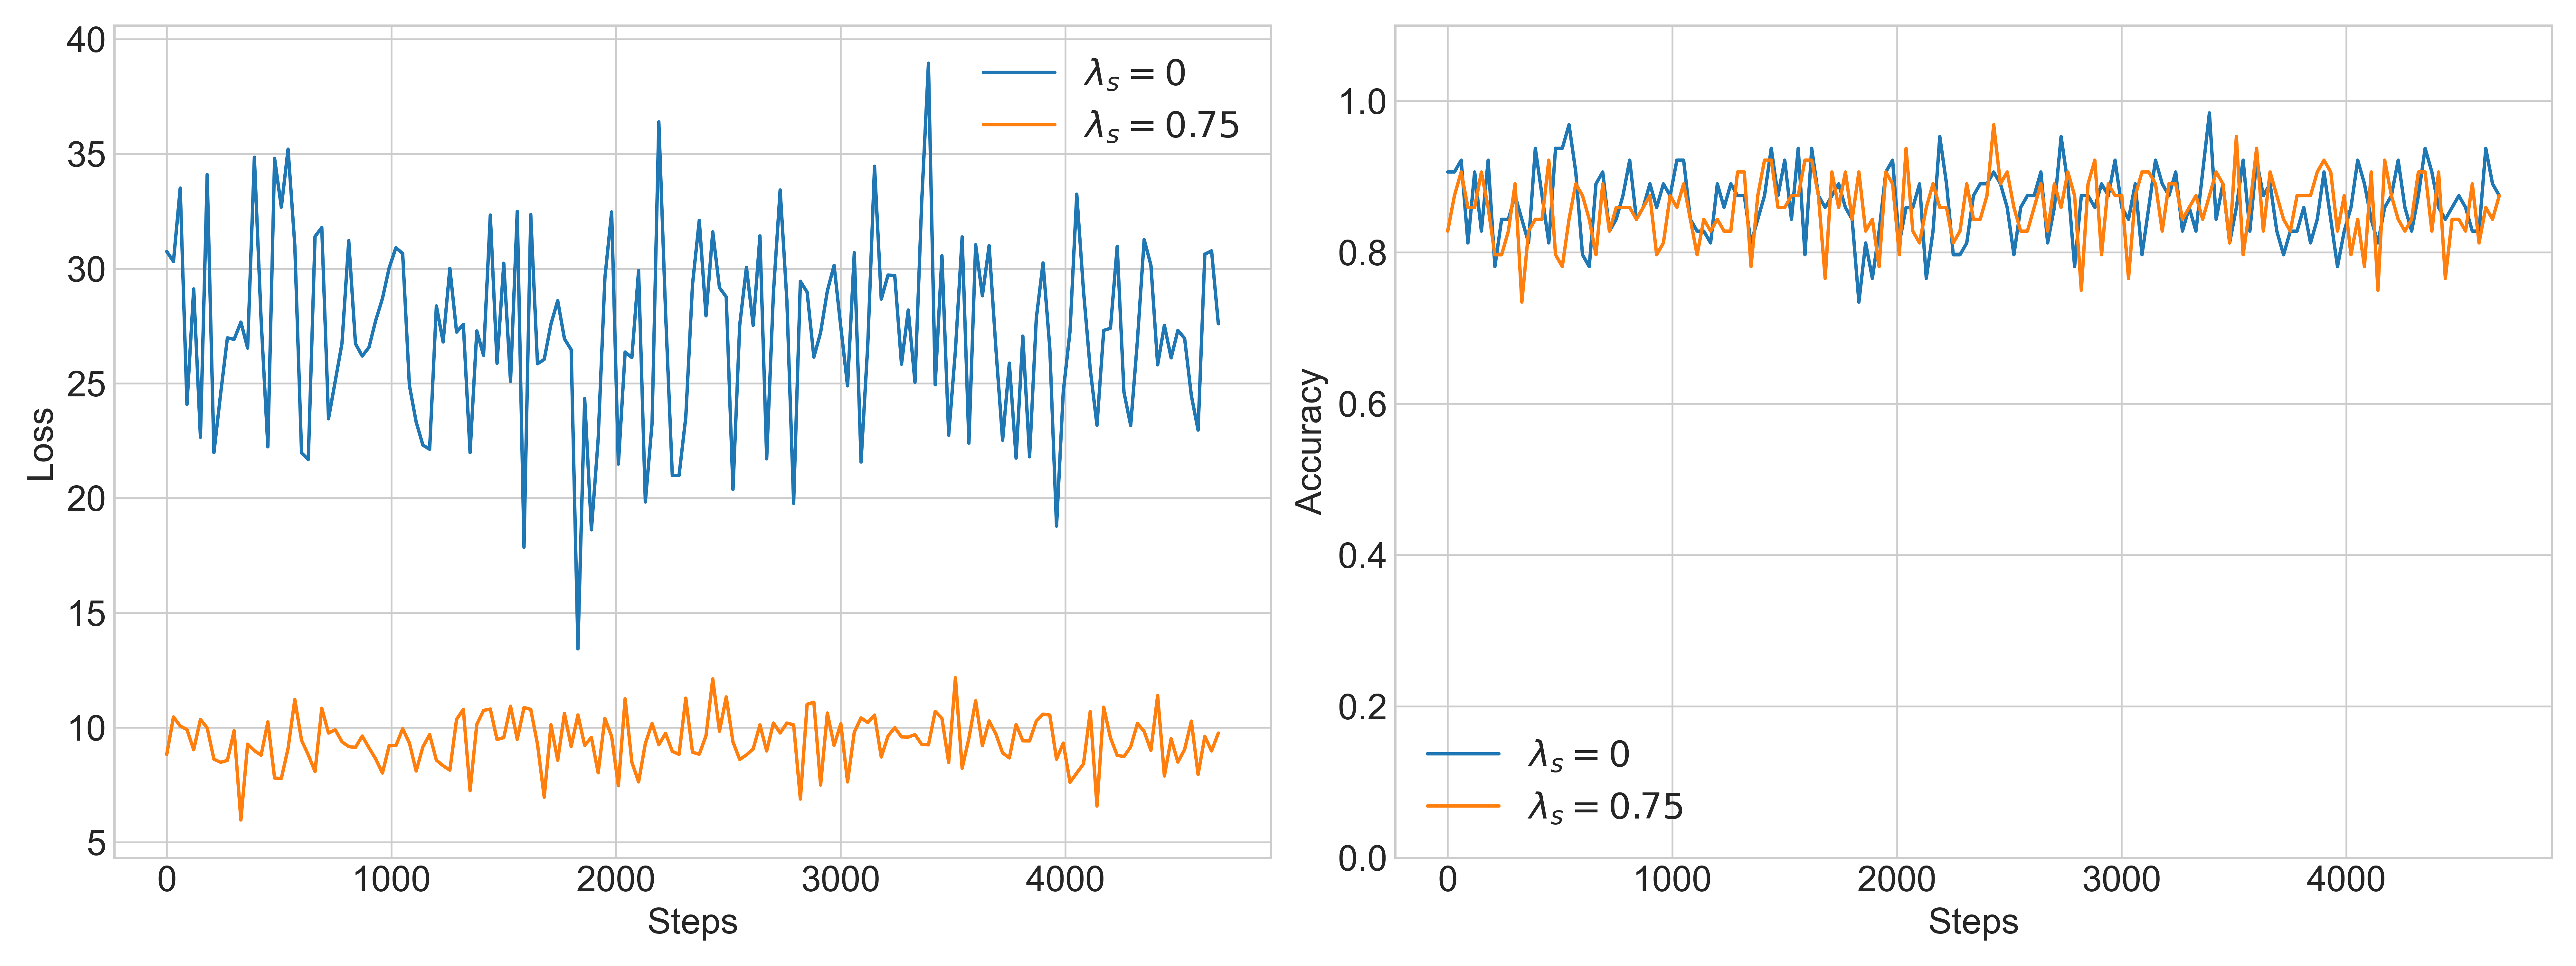
\includegraphics[width=\linewidth]{images/coco_fixedListener_baseline_random_0_075_losses.png}
	\caption{Training results of the MS COCO experiment with a fixed listener (pure decoding, $\lambda_s=0$ vs. $\lambda_s=0.75$). Left: Total speaker training loss. Right: Listener training accuracy.}
	\label{fig:coco_fixed_listener_speaker_loss_listener_acc_075}
\end{figure}

The training and testing procedures were identical to previously described random image pairs experiments. The training dynamics can be seen in Figure \ref{fig:coco_fixed_listener_speaker_loss_listener_acc_075}. They indicate that the task success based training signal was not strong enough in order to visibly improve the task performance beyond literal message interpretation, because the listener's accuracy did not improve beyond the accuracy in responding to the pretrained speaker (right plot). The speaker's policy also did not visibly converge (left plot). 
This is confirmed by the listener test accuracy of 0.881 in Table \ref{tab:coco_drift_metrics_basic}, which additionally indicates that the reference game success is at least partly carried by speaker-listener co-adaptation, since the accuracy decreased by 0.072 compared to the experiment with a jointly trained listener. 

Turning to the language drift metrics in Table \ref{tab:coco_drift_metrics_basic}, it can be observed that training the speaker with a fixed listener indeed mitigated structural and semantic drifts, compared to training with a joint listener (``MS random, fixed listener, $\lambda_s=0.75$'' line~vs.~``MS baseline, random, $\lambda_s=0.75$'' line compared to the ``Pretrained MS speaker''). Consistent with intuitions, the mitigation was stronger for the semantic drift than for structural drift---the log likelihood was 4.192 higher for the former and 1.502 higher for the latter for the fixed listener experiment, compared to the joint one (Tab.~\ref{tab:coco_drift_metrics_basic}). Based on the drift dynamics during the training (Fig.~\ref{fig:coco_fixed_listener_075_str_sem_drift}), one could, however, hypothesize that with longer training, the semantic drift might increase (based on the slightly visible negative trend in the right plot). Consistent with the effects of the fixed listener on the apparent absence of functional speaker improvement discussed above, the discrete overlap did not increase compared to the pretrained speaker (and even decreased by 0.152). The continuous overlap did not change compared to the pretrained speaker. The image caption evaluation metrics in Table \ref{tab:eval_metrics_refgame} suggest that the speaker's messages diverged from the ground truth a little stronger than for the pretrained speaker and the joint listener-trained speaker, but the differences seem negligible.
\begin{figure}
	\centering
	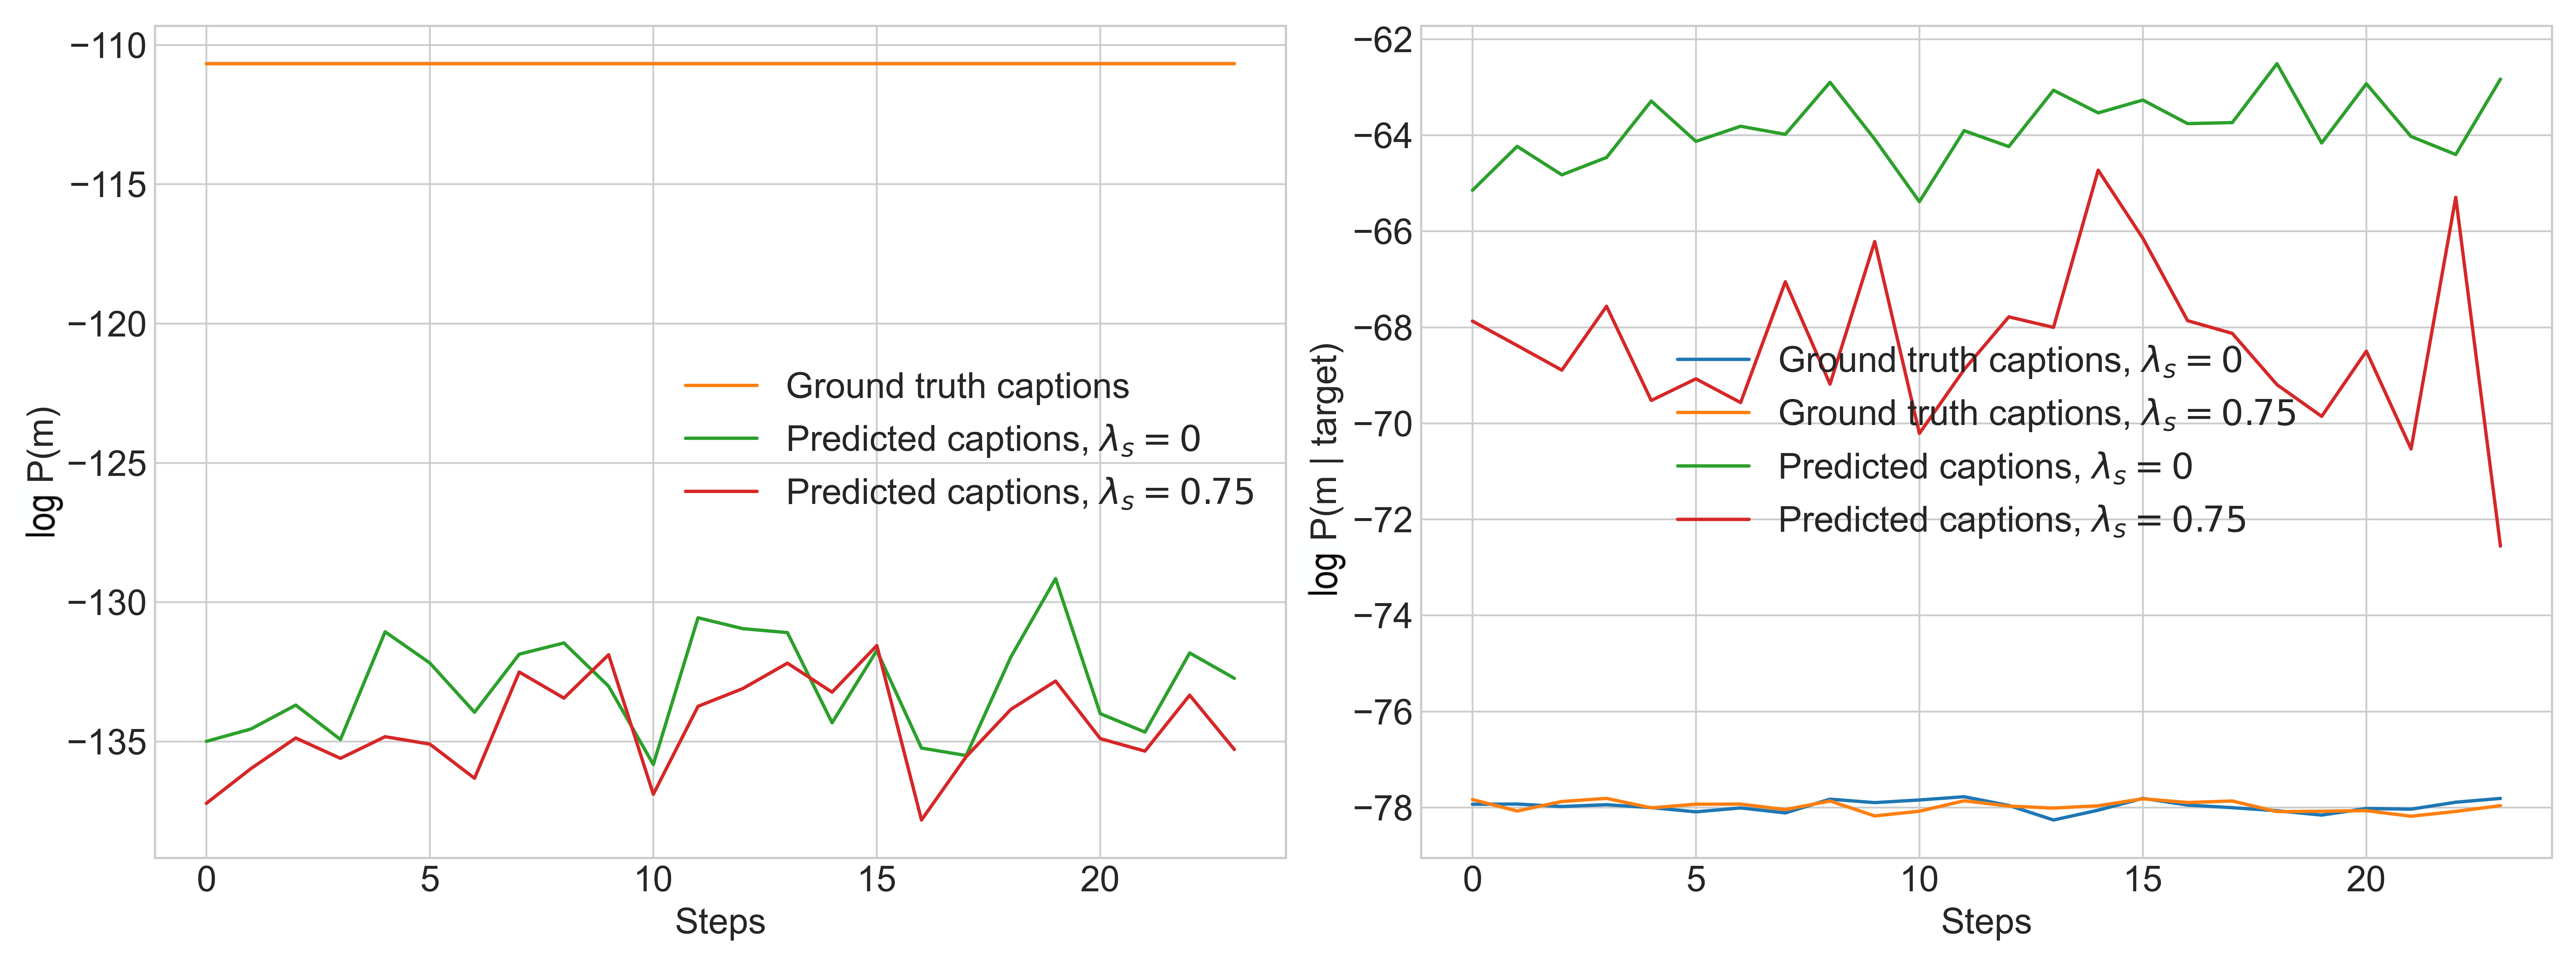
\includegraphics[width=\linewidth]{images/coco_fixedListener_structural_semantic_drift_4000_pure_0_075_random.png}
	\caption{Drift dynamics computed during reference game training with the fixed listener on MS COCO (pure decoding, $\lambda_s=0$ vs. $\lambda_s=0.75$). Higher values indicate less drift. Left: Structural drift of ground truth and predicted captions under the pretrained LM. Right: Semantic drift of ground truth and predicted captions under the pretrained speaker model.}
	\label{fig:coco_fixed_listener_075_str_sem_drift}
\end{figure}

In order to investigate whether task improvement can be achieved without speaker-listener co-adaptation when a stronger functional learning signal is present, a second experiment with $\lambda_s=0$ (i..e, functional learning only) was conducted. While no improvement in terms of task performance is apparent visually (Fig,~\ref{fig:coco_fixed_listener_speaker_loss_listener_acc_075}), there was a little increase in terms of listener test accuracy to 0.888 (Tab.~\ref{tab:coco_drift_metrics_basic}). Furthermore, Table \ref{tab:coco_drift_metrics_basic} indicates that under stronger functional constraints, language drift was mitigated even better, compared to the $\lambda_s = 0.75$ fixed listener. More precisely, structural drift was lower, even outperforming the pretrained speaker. Similarly, semantic drift also narrowly improved beyond both the pretrained and the $\lambda_s = 0.75$ speakers. 
The overlap metrics also slightly improved or remained constant compared to both the $\lambda_s=0.75$ experiment, the jointly trained listener-speaker experiment and the pretrained speaker. These results suggest that when removing the agent co-adaptation, a strong enough functional training signal might yield more discriminative captions which mention more target than distractor features. 

To sum up, the data supports \textbf{H6} for the MS COCO experiment, but also strongly suggests that the functional signal available under the functional loss weight of 0.25 is not sufficient in order to visibly fine-tune the speaker for the task. When increasing the strength of the functional signal from the listener by setting $\lambda_s$ to 0, a tangiable improvement of language drift can be observed, indicating that both grounding and the structure expected by the listener positively affect the speaker.

\subsection{MS COCO: Greedy Decoding Experiments}
\label{expt:coco_greedy}
\begin{table}[]
	\begin{tabularx}{\linewidth}{|X|l|l|X|X|X|X|}
		\hline
			\textbf{Model name}                                    & \textbf{log $P(m)$} & \textbf{log $P(m \mid i)$} & \textbf{Overlap (d)} & \textbf{Overlap (c)} & \textbf{Acc. (random)} & \textbf{Acc. (similar)} \\ \hline
			 Baseline random pairs, fixed listener, pure decoding   &     -138.500         &         -74.988               &       1.059            &      0.001               &       0.865          &                \\ \hline
			 Baseline random pairs, fixed listener, greedy decoding   &     -100.674     &         -36.419              &       1.400       &      0.005             &       0.814          &                \\ \hline
			 Baseline random pairs, pure decoding   & -136.114        &      -72.959            &       1.065          &      0.002               &       0.55          &                \\ \hline
			 Baseline random pairs, greedy decoding   &-100.187      &    -35.910            &       1.355          &      0.006            &       0.544         &                \\ \hline
			 Baseline similar pairs, pure decoding   &     -137.491& -77.898    & 0.198    &   -0.005    &            &  0.542        \\ \hline
			 Baseline similar pairs, greedy decoding   &   -101.436  &      -38.911        &     0.044   &     0.003     &            &     0.565           \\ \hline
			 
	\end{tabularx}
\caption{\label{tab:coco_greedy}Language drift metrics and listener test accuracies (``Acc.'') on MS COCO experiments conducted with greedy decoding.}
\end{table}

Finally, as explained in the introduction (see Section~\ref{model_pretraining}), another factor which may influence the performance of the speaker is the decoding strategy. While pure decoding was chosen as the main strategy, this section looks at representative sample experiments employing \emph{greedy} decoding. That is, at each timestep of the generation, the speaker picked the token with the highest probability given the images and preceeding tokens in order to continue her message. 

For gathering representative results, the baseline experiment (random pairs, joint listener, $\lambda_s=0.75$), the similar pairs experiment (joint listener, $\lambda_s=0.75$) and a fixed listener experiment (random pairs, $\lambda_s=0.75$) were replicated with the greedy decoding strategy. Training results in Figure~\ref{fig:coco_greedy_baseline} indicate that for the joint listener experiments, the agents failed to learn the reference game (i.e., their training performance remained at chance level 0.5). Since the speaker and the fixed listener were able to play the game, the reason for failure in the other two experiments most likely was the inability to ground the joint listener. That is, the listener could not pick up how the speaker described the target, both for random and similar target-distractor pairs. This is corroborated by nearly chance-level listener test accuracy (Tab.~\ref{tab:coco_greedy}). For all three experiments, the test performance with greedy decoding on the test set was compared to test performance with pure decoding on the same set. 
\begin{figure}
	\centering
	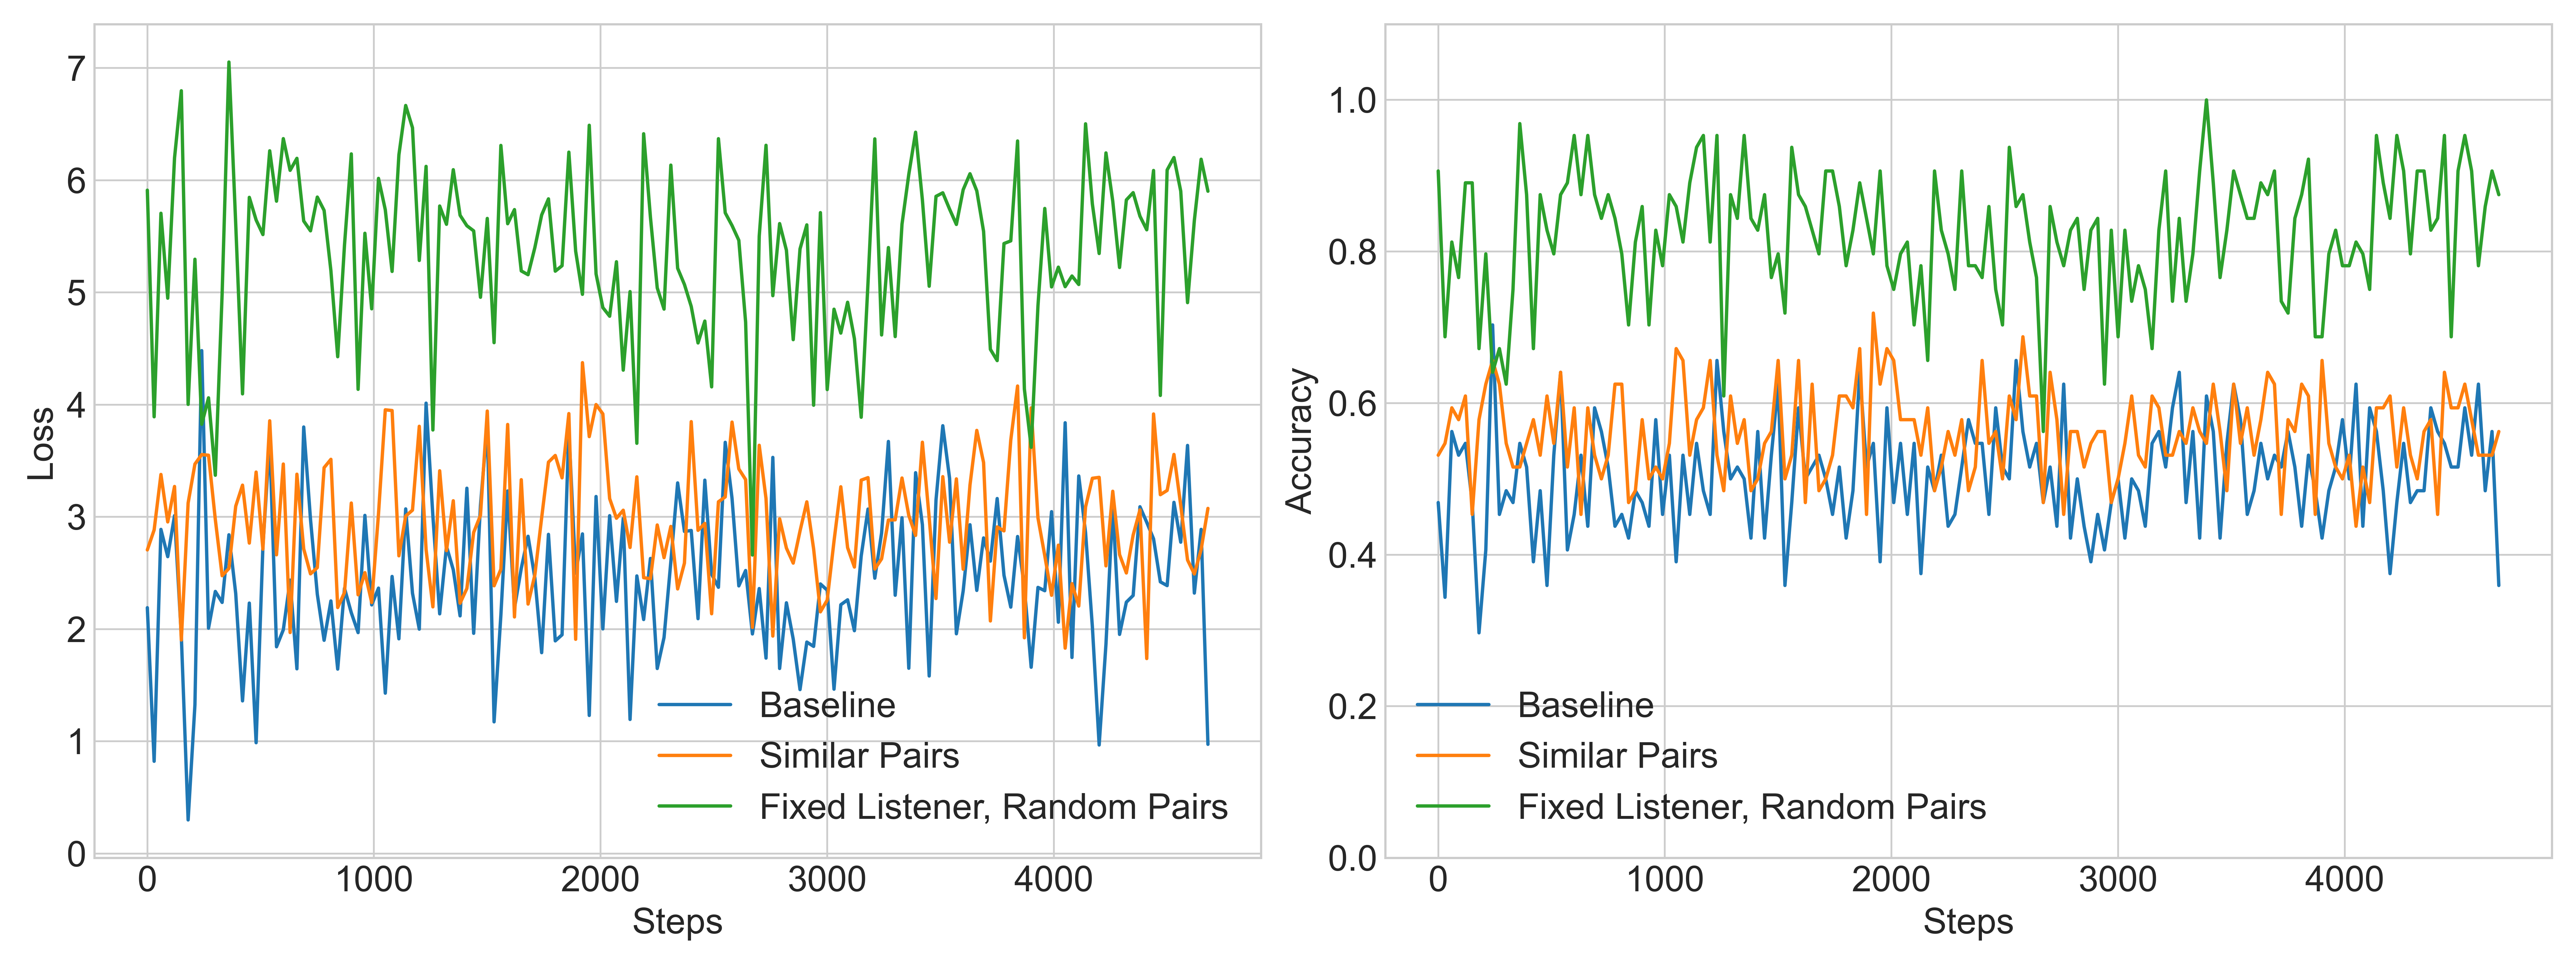
\includegraphics[width=\linewidth]{images/coco_greedy_all_075_losses.png}
	\caption{Training results of three experiment with greedy decoding on MS COCO ($\lambda_s = 0.75$): baseline random pairs, with a fixed listener on random pairs, and with a joint listener on similar pairs. Left: Total speaker training loss. Right: Listener training accuracy.}
	\label{fig:coco_greedy_baseline}
\end{figure} 
\pt{def add example generations here}
Interestingly, although the messages seem to be unsuitable for learning the reference game, their semantic and structural drifts during training were well \emph{above} the drifts of both ground truth captions and the pure decoding experimental results (Fig.~\ref{fig:coco_greedy_drifts}~vs.,~e.~g.,~Fig.~\ref{fig:coco_baseline_str_sem_drift_all}). Drift values on the test set clearly indicate that using greedy decoding led to messages with lower structural and semantic drift values. Intuitively, this makes sense because greedy decoding selected the highest probability tokens, resulting in overall higher message probabilities under the pretrained models measuring drift. Even the overlap metrics were higher under greedy test decoding compared to pure test decoding for the random pairs experiments, suggesting that it was not the absence of discriminative words that potentially was responsible for the task failure of the joint listeners. Only for similar pairs greedy decoding might not have been able to retrieve critical discriminative words. This could be because there were less options among which discriminative words could be selected, and these were simply ignored due to lower probability.
\begin{figure}
	\centering
	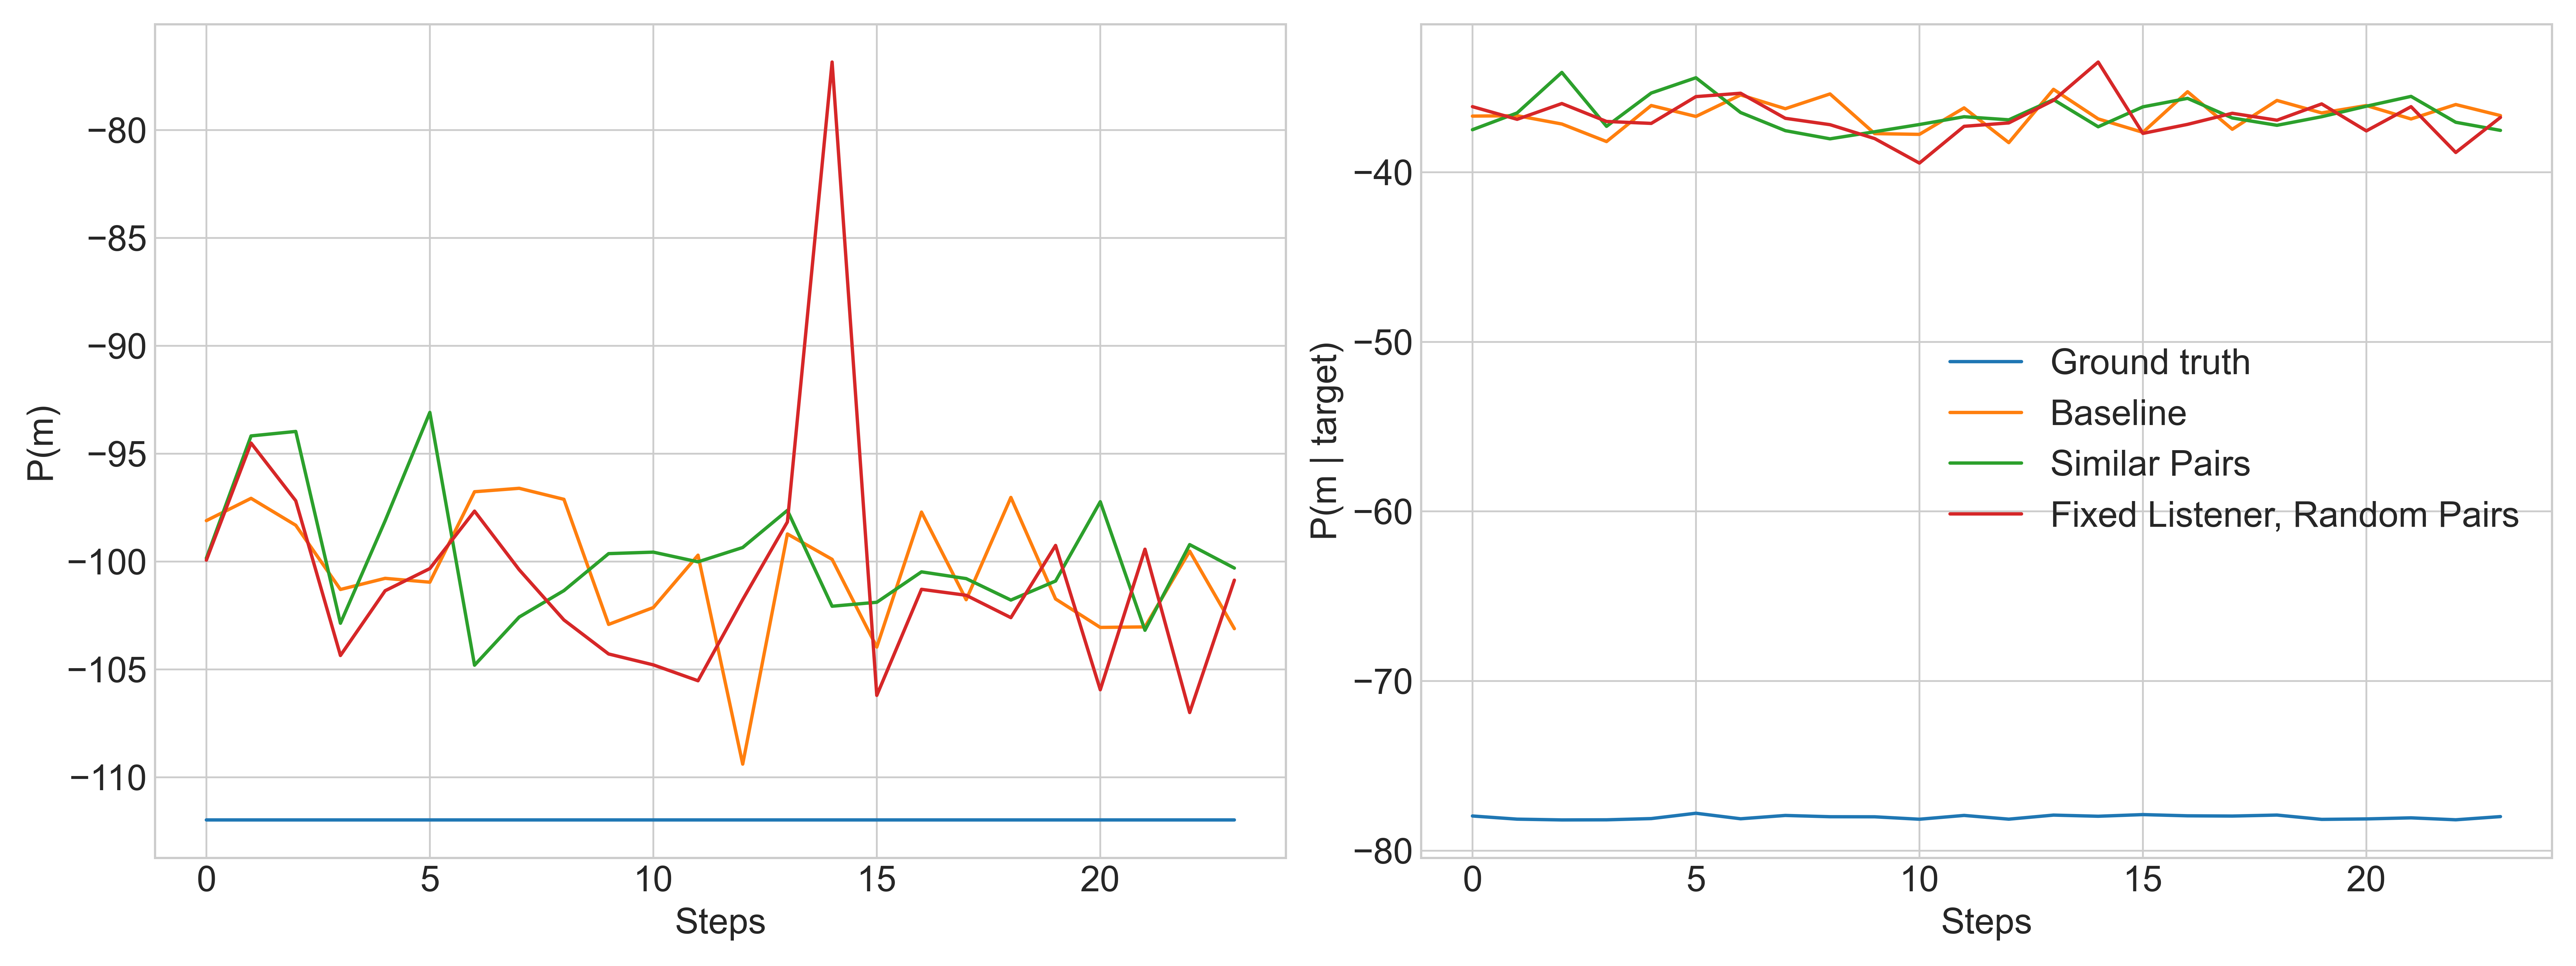
\includegraphics[width=\linewidth]{images/coco_structural_semantic_drift_greedy_all_4000_pure_075.png}
	\caption{Drift computed during training of three MS COCO experimens, using greedy speaker decoding ($\lambda_s = 0.75$). Left: Strucutral drift of ground truth and predicted captions under a pretrained LM. Right: Semantic drift of ground truth and predicted captions under the pretrained speaker model.}
	\label{fig:coco_greedy_drifts}
\end{figure} 

The most plausible explanation for the task failure might be that the speaker was pretrained using pure decoding, yet fine-tuned on the reference game using greedy decoding. This change in strategy might have been disadvantageous for the learned conditioning on the images, hindering the listener from successful grounding. Therefore, for more comprehensive results, these experiments should be replicated using a greedily pretrained speaker. Another potential source of failure might be the observation that greedy decoding agents tend towards word repetitions \parencite[cf.][]{lee2019countering}. While the fixed listener might have been able to ignore the repetitions and attend to critical content words, it seems that these repetitions might have overriden the critical grounding signal for the jointly trained listeners. Comparing the fixed listener test semantic drift to the same value in the pure decoding experiment (Tab.~\ref{tab:coco_greedy}~vs.~Tab.~\ref{tab:coco_drift_metrics_basic}), it is visible that the fixed listener did not mitigate semantic drift in the greedy decoding experiment that well, further supporting that greedy decoding fine-tuning might have corrupted the speaker's grounding from pretraining. 
These trends also overpowered differences in the visual input, yielding similar results on random and similar pairs.
Overall, this combination of low drifts with a failure to learn the reference game indicates that the drift values alone are not representative of the agents' success, and factors which are not captured by the metrics may play a critical role for functional success, especially when training the listener agent from scratch. The results also suggest that the decoding strategy is a critical component of the system which may need to be held constant between pretraining and task-based fine-tuning, which may imply limitations when using pretrained models for fine-tuning on downstream tasks.

\pt{Overall summary of MS COCO experiments goes here.}
Summarizing the experiments on the MS COCO dataset, it was shown that artificial agents could learn to play a reference game on real-world images, while using natural language. Their learning speed in the game crucially depended on the discriminability of the target among distractors. Consistent with the literature, the agents were subject to structural and semantic language drift which was best mitigated by training the speaker against a fixed listener, but, at the same time, was pre-determined by the quality of the pretrained speaker. The decoding strategy was shown to be an important factor for the drift. Finally, it was shown that task-conditional fine-tuning of the speaker's messages might require longer training, although even a few epochs were sufficient for the speaker to adjust the granularity of her messages according to the complexity of the image pairs.

\subsection{3Dshapes: Baseline Experiments}
\label{expt:3dshapes_baseline}

The goal of these experiments was to investigate the importance of presenting exhaustive example captions to the model during training for potentially mitigating language drift. To this end, the 3Dshapes dataset was annotated with exhaustive captions (see Section \ref{ds:3dshapes}) and various experiments were conducted. %Additionally, these experiments focus on investigating the model's potential to generate informative captions, without being overinformative. \pt{spell out the operationalization}

\begin{table}[] 
	\begin{tabularx}{\textwidth}{|X|l|l|X|X|X|X|}
		\hline
		\textbf{Model name}                                    & \textbf{log $P(m)$} & \textbf{log $P(m \mid i)$} & \textbf{Overlap (d)} & \textbf{Overlap (c)} & \textbf{Acc. (random)} & \textbf{Acc. (similar)} \\ \hline
		Ground truth exh.       &      -164.752            &         -101.329               &       6.881             &      0.023               &                 &                \\ \hline
		Pretrained 3D exh. speaker                            &       -195.753            &         -145.638               &        5.428              &      0.001                & 0.953 (random listeners)                 & 0.808 (similar listeners)                 \\ \hline
		3D Baseline, random, $\lambda_s = 0$ &       -195.420            &    -147.938                    &           5.294            &      -0.002                &                 0.979                         &                                           \\ \hline
		3D Baseline, random, $\lambda_s = 0.25$     &     -196.811              &       -140.862                 &          5.104            &       -0.006               &          0.969                                &                                           \\ \hline
		3D Baseline, random, $\lambda_s = 0.5$   &         -196.722          &        -144.301                &        4.968              &          0.002            &                  0.971                      &                                           \\ \hline
		3D Baseline, random, $\lambda_s = 0.75$  &       -195.495        &           -147.313           &          5.247            &         0.001             & 0.979                                    &                        0.959                   \\ \hline
		3D Baseline, random, $\lambda_s = 1$   &      -196.019             &            -137.456             &        5.257              &          -0.005            &              0.979                            &                                           \\ \hline
		3D fixed listener, random, $\lambda_s = 0$&      -196.111          &     -136.134                  &             5.339         &         -0.008            &                   0.927                      &                                           \\ \hline
		3D fixed listener, random, $\lambda_s = 0.75$&      -194.990          &     -140.483                  &             5.298         &         -0.003            &                   0.927                      &                                           \\ \hline
		3D fixed listener, similar fixed, same test &  -198.434       &      -147.121     &     2.892 &    0.025         &        &      0.744          \\ \hline
		3D fixed listener, similar fixed, diff. test & -198.188   & -143.309      & 2.187   & 0.045    &    &   0.822     \\ \hline
	\end{tabularx}
	\caption{\label{tab:3dshapes_drift_metrics_basic_baseline} Language drift metrics and listener test accuracies (``Acc.'') on different pairs. 
		``Baseline'' refers to the setup wherein the listener is trained jointly with the speaker, using pure decoding. 3D refers to the 3DShapes dataset. ``Random'' refers to speakers trained on random target-distractor pairs; ``similar'' refers to speakers trained on similar pairs. ``Overlap (d)'' refers to the discrete overlap metric, ``overlap (c)'' to continuous overlap. The speakers trained on similar pairs are still tested on random pairs.}
\end{table}

\begin{figure}[h]
	\centering
	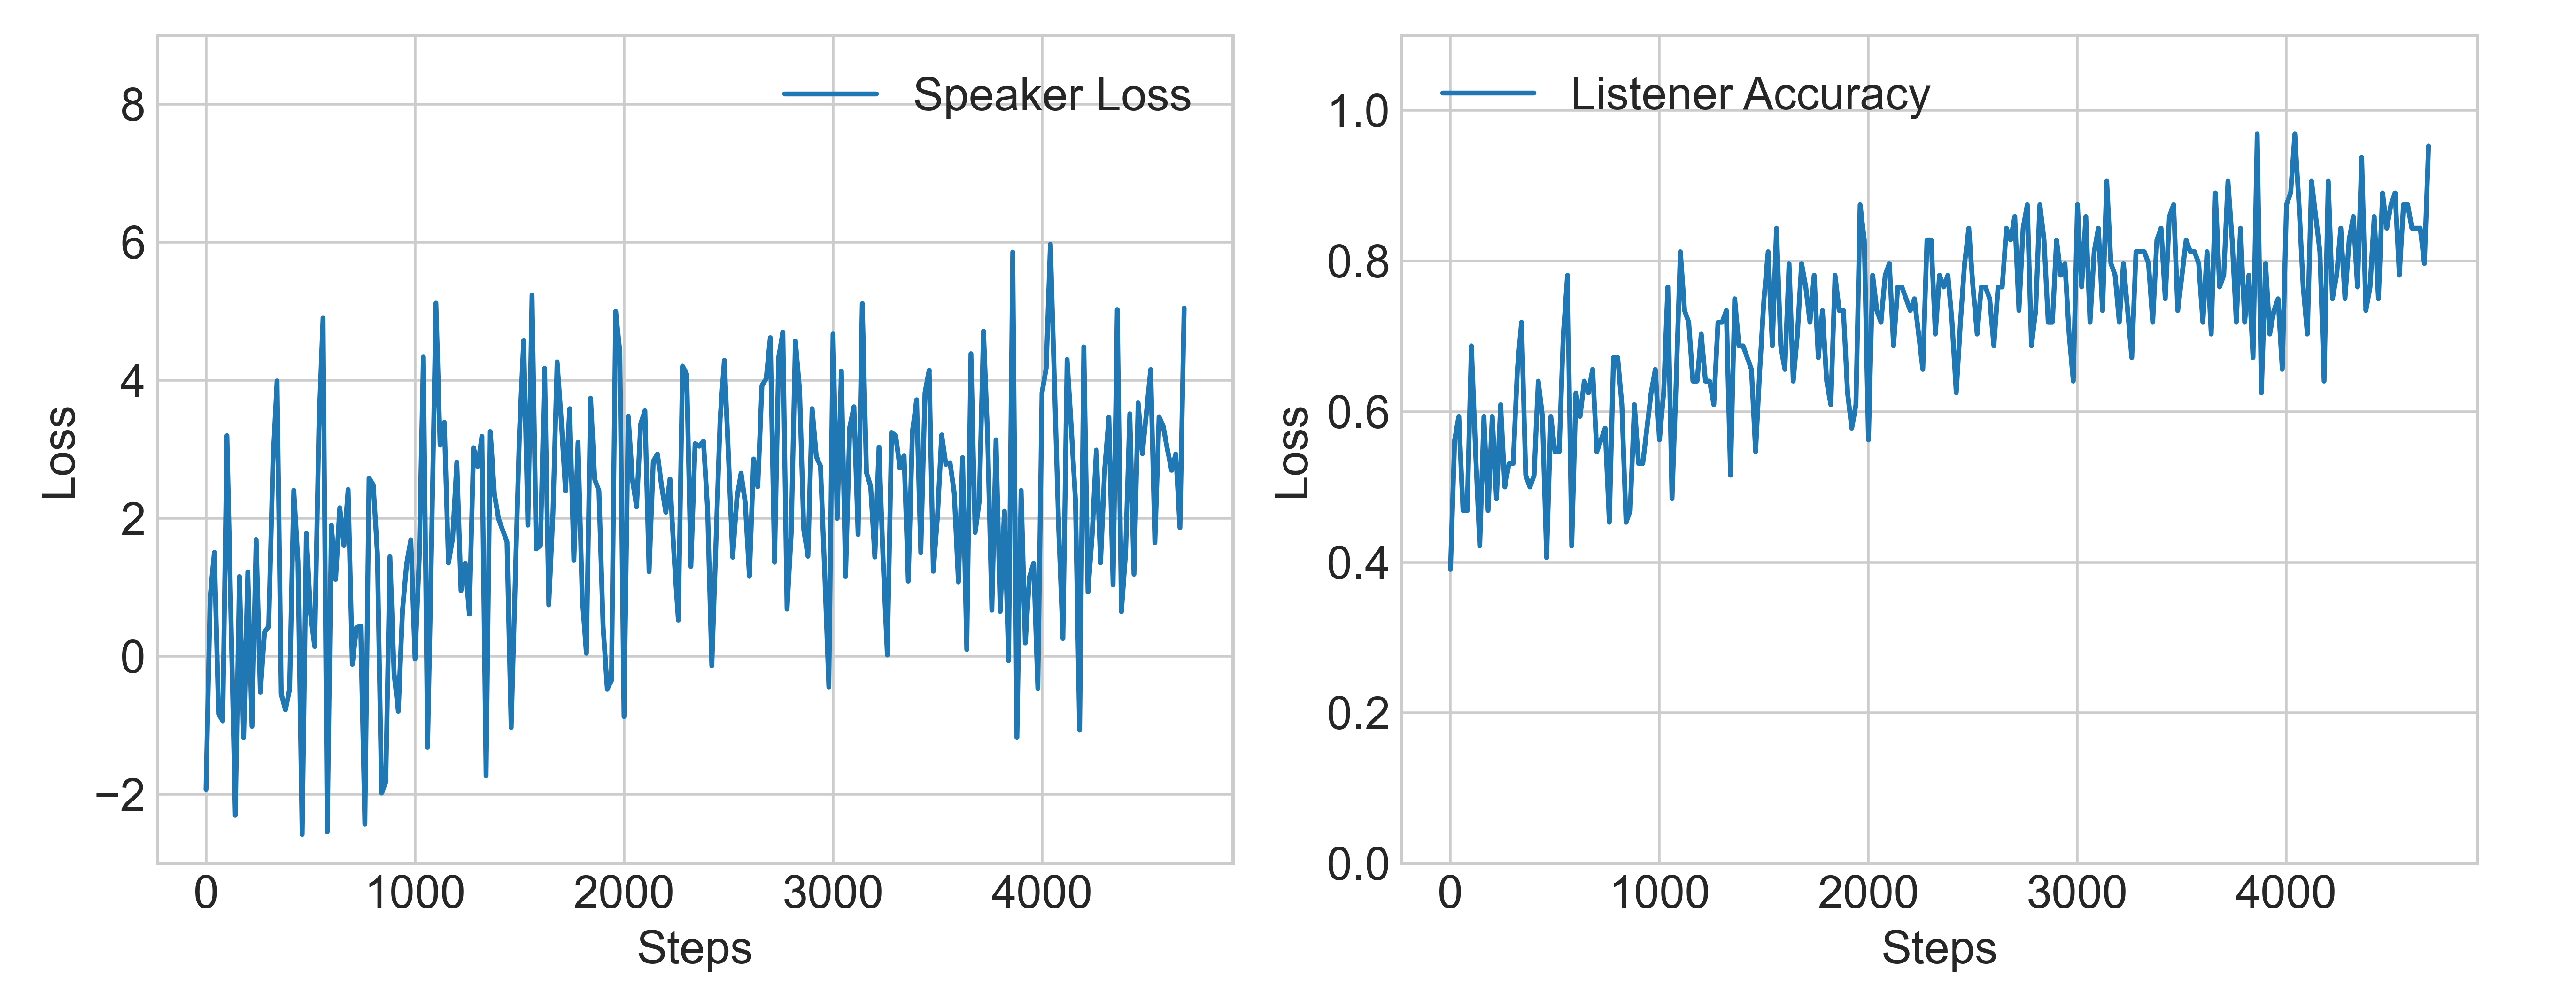
\includegraphics[width=\linewidth]{images/3dshapes_refgame_49_pure_075.png}
	\caption{Training results of the baseline 3Dshapes experiment (pure decoding, random pairs, $\lambda_s = 0.75$). Left: Total speaker training loss. Right: Listener training accuracy.}
	\label{fig:3dshapes_baseline_075_speaker_loss_listener_acc}
\end{figure}

\begin{figure}
	\centering
	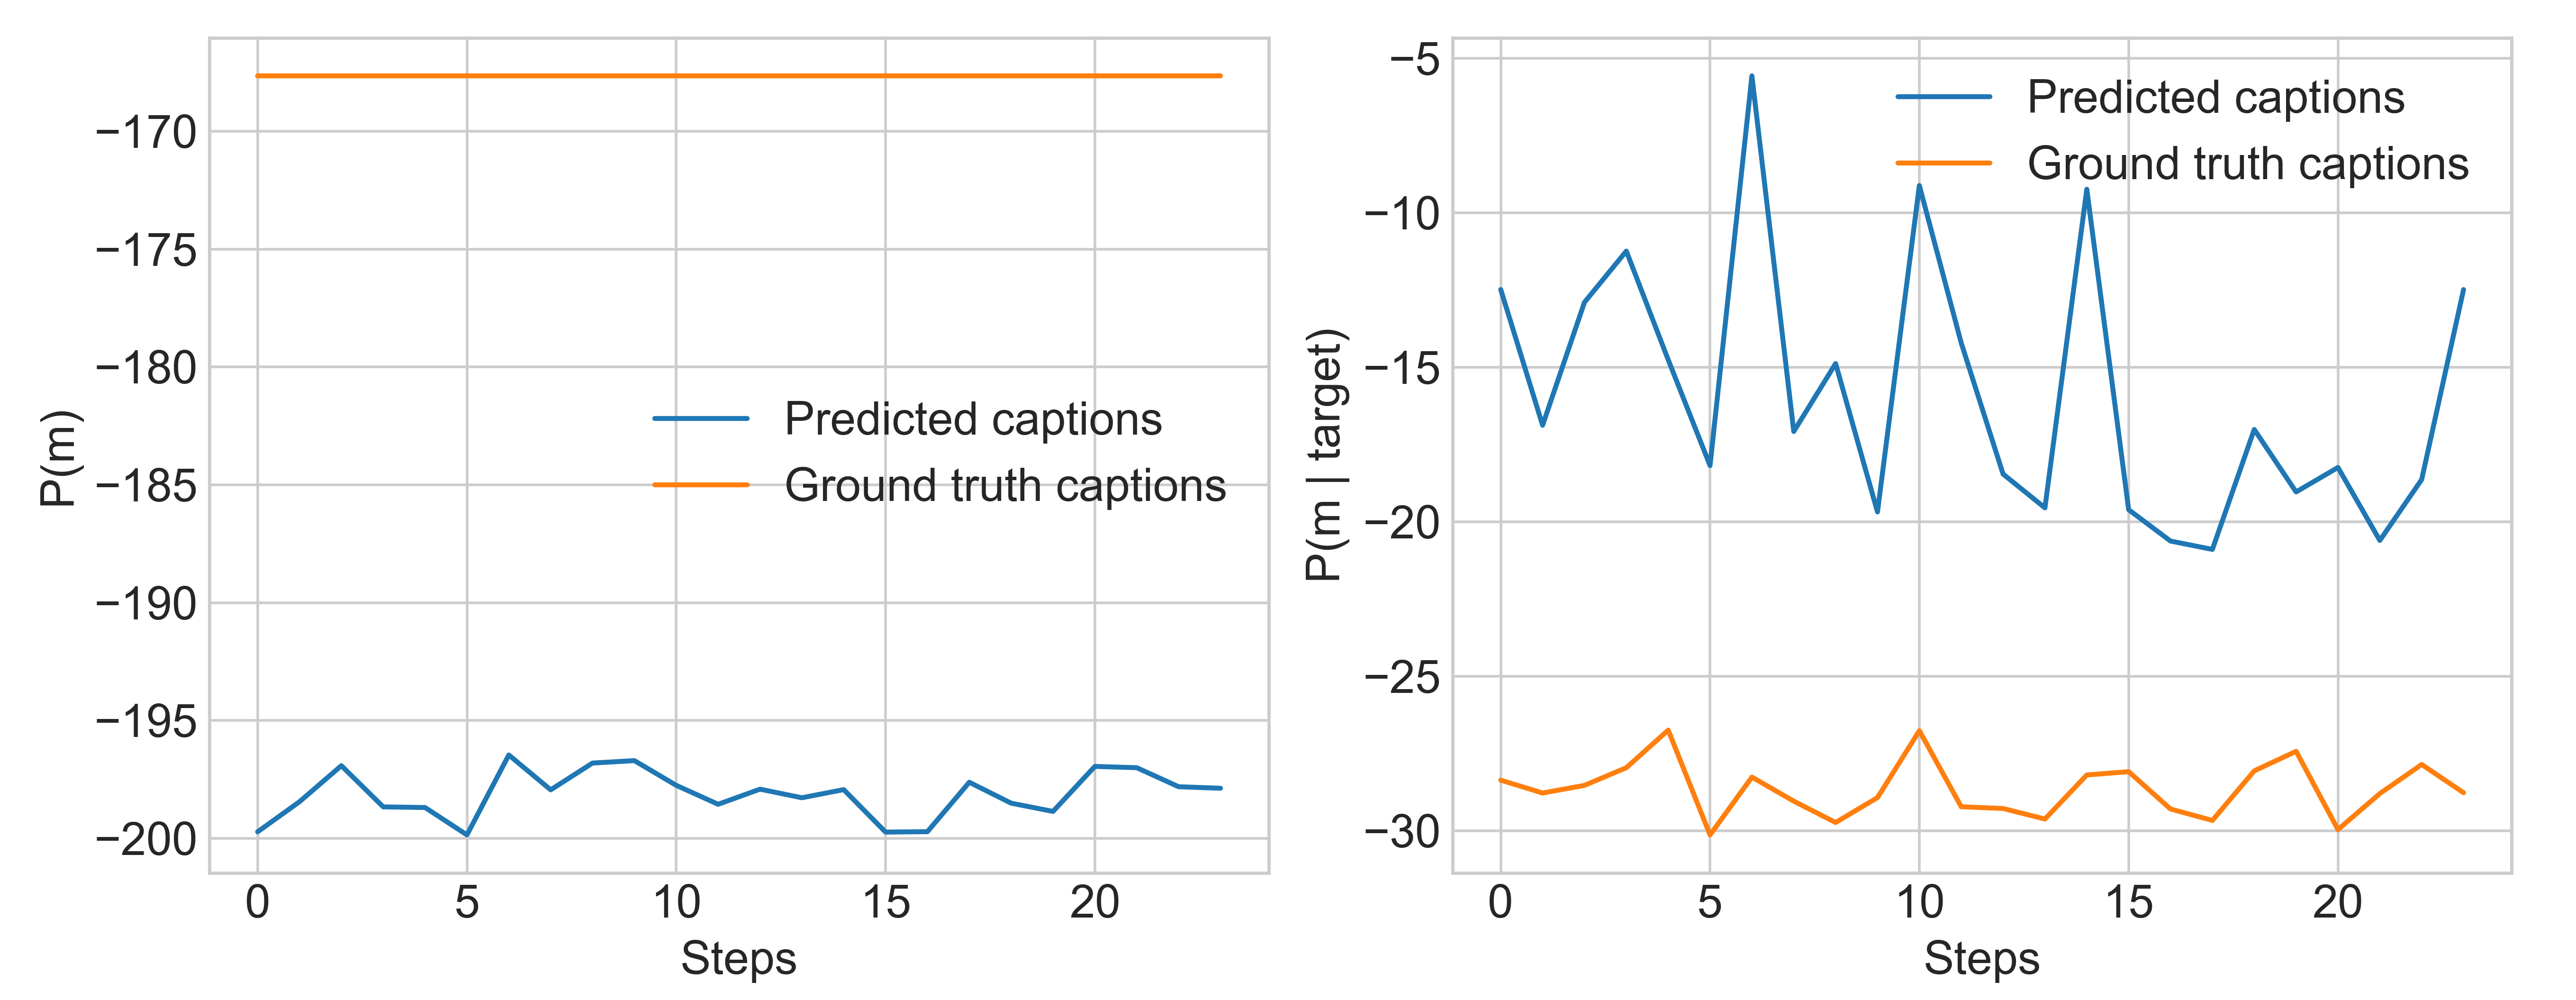
\includegraphics[width=\linewidth]{images/3dshapes_structural_semantic_drift_49_pure_075_random.png}
	\caption{Drift values computed during training in the baseline 3Dshapes experiment (pure decoding, $\lambda_s = 0.75$). Higher values are better. Left: Strucutral drift of ground truth and predicted captions under a pretrained LM. Right: Semantic drift of ground truth and predicted captions under the pretrained speaker model.} 
	\label{fig:3dshapes_baseline_075_str_drift}
\end{figure}

First, a baseline experiment with pure decoding and $\lambda_s = 0.75$ was conducted.
The configurations as well as the training procedure of this experiment matched the general configurations of the MS COCO baseline experiment in Section \ref{expt:coco_baseline}. The training dynamics of this baseline experiment can be seen in Figure \ref{fig:3dshapes_baseline_075_speaker_loss_listener_acc}. Interestingly, compared to the reference game on MS COCO (see Fig.~\ref{fig:coco_baseline_075_speaker_loss_listener_acc}, right), the training of the listener did not visibly converge faster, although the action space (i.e., vocabulary space---49 tokens for 3Dshapes~vs.~4054 tokens for MS COCO) that the speaker had to learn was significantly smaller. 
 
Supporting the visual results, Table \ref{tab:3dshapes_drift_metrics_basic_baseline} shows that the agents successfully learned the reference game---the listener test accuracy was 0.979, even outperforming the MS COCO baseline experiment. Accuracy also improved by 0.026 compared to the pretrained speaker. 
Supporting \textbf{H2}, slight semantic drift can be observed in this experiment---the average conditional log likelihood of the captions generated by the trained speaker decreased by 1.675, compared to the captions produced by the pretrained speaker. In contrast to the MS COCO baseline experiment, \textbf{H1} was not supported in this experiment, as the average log likelihood under the pretrained LM actually increased by 0.258, compared to the pretrained speaker (Table~\ref{tab:3dshapes_drift_metrics_basic_baseline}).
 
The dynamics of structural and semantic drifts during training can be seen in Figure \ref{fig:3dshapes_baseline_075_str_drift}; these are in line with the validation results (Tab.~\ref{tab:3dshapes_drift_metrics_basic_baseline}).\footnote{Due to a coding mistake, the language drift computed during training of the baseline random pairs experiment on 3Dshapes was computed on 50 images from the training dataset, not the validation dataset. Furthermore, semantic drift was computed using greedy decoding, and only on one image pair.} 
Interestingly, the magnitude of the structural drift values was much higher for 3Dshapes than for MS COCO, indicating that the generated captions might in general be less likely under the pretrained Transformer XL model used for the computation. Similarly, the higher magnitude of the semantic drift values indicates that the speaker was generally uncertain when generating captions for these images. This could partly be due to the difference in the 3Dshapes data distribution compared to the ImageNet data on which the visual module of the speaker was pretrained. Additionally, this could be due to the variability of the syntactic structures of the generated ground truth sentences (cf. Section \ref{ds:3dshapes}). 

Turning to the overlap metrics in Table~\ref{tab:3dshapes_drift_metrics_basic_baseline}, against predictions, the discrete overlap decreased by 0.181 tokens on average, compared to the pretrained speaker, while the continuous overlap did not change. Similarly to MS COCO, the overlap was also generally lower than for the ground truth captions, indicating that the trained speaker's captions might not cover all features mentioned in the exhaustive ground truth captions. An interesting direction for future work is the investigation of potential regularities in the type of feature descriptions omitted by the speaker. A further interesting observation is that the difference in the discrete overlaps between the baseline speaker and the ground truth captions was much smaller in the 3Dshapes experiment (1.634), compared to MS COCO (7.95). This might be an indication of a more robust grounding of the 3Dshapes speaker mentioning more of the features contained in the images, compared to the MS COCO speaker, which might be attributed to the significantly smaller action space of the former. In sum, \textbf{H3} was not supported by the data from the 3Dshapes baseline experiment.

\pt{Linear regressions will be computed on the drift values collected during the training.}

Additionally, the fine-tuned speaker was evaluated with standard image captioning metrics. Table \ref{tab:eval_metrics_refgame} shows that caption quality marginally decreased with respect to almost all metrics except for CIDEr and BLEU-1. Noteworthily, in contrast to the language drift metrics, these metrics are significantly higher for the 3Dshapes dataset compared to MS COCO, indicating that the generated captions have a relatively high overlap with ground truth captions. This calls for careful consideration of the pretraining datasets and their similarity to the target dataset when using available pretrained models like ResNet and Transformer XL.

\subsubsection{Varying Structural Loss}

\begin{figure}[h]
	\centering
	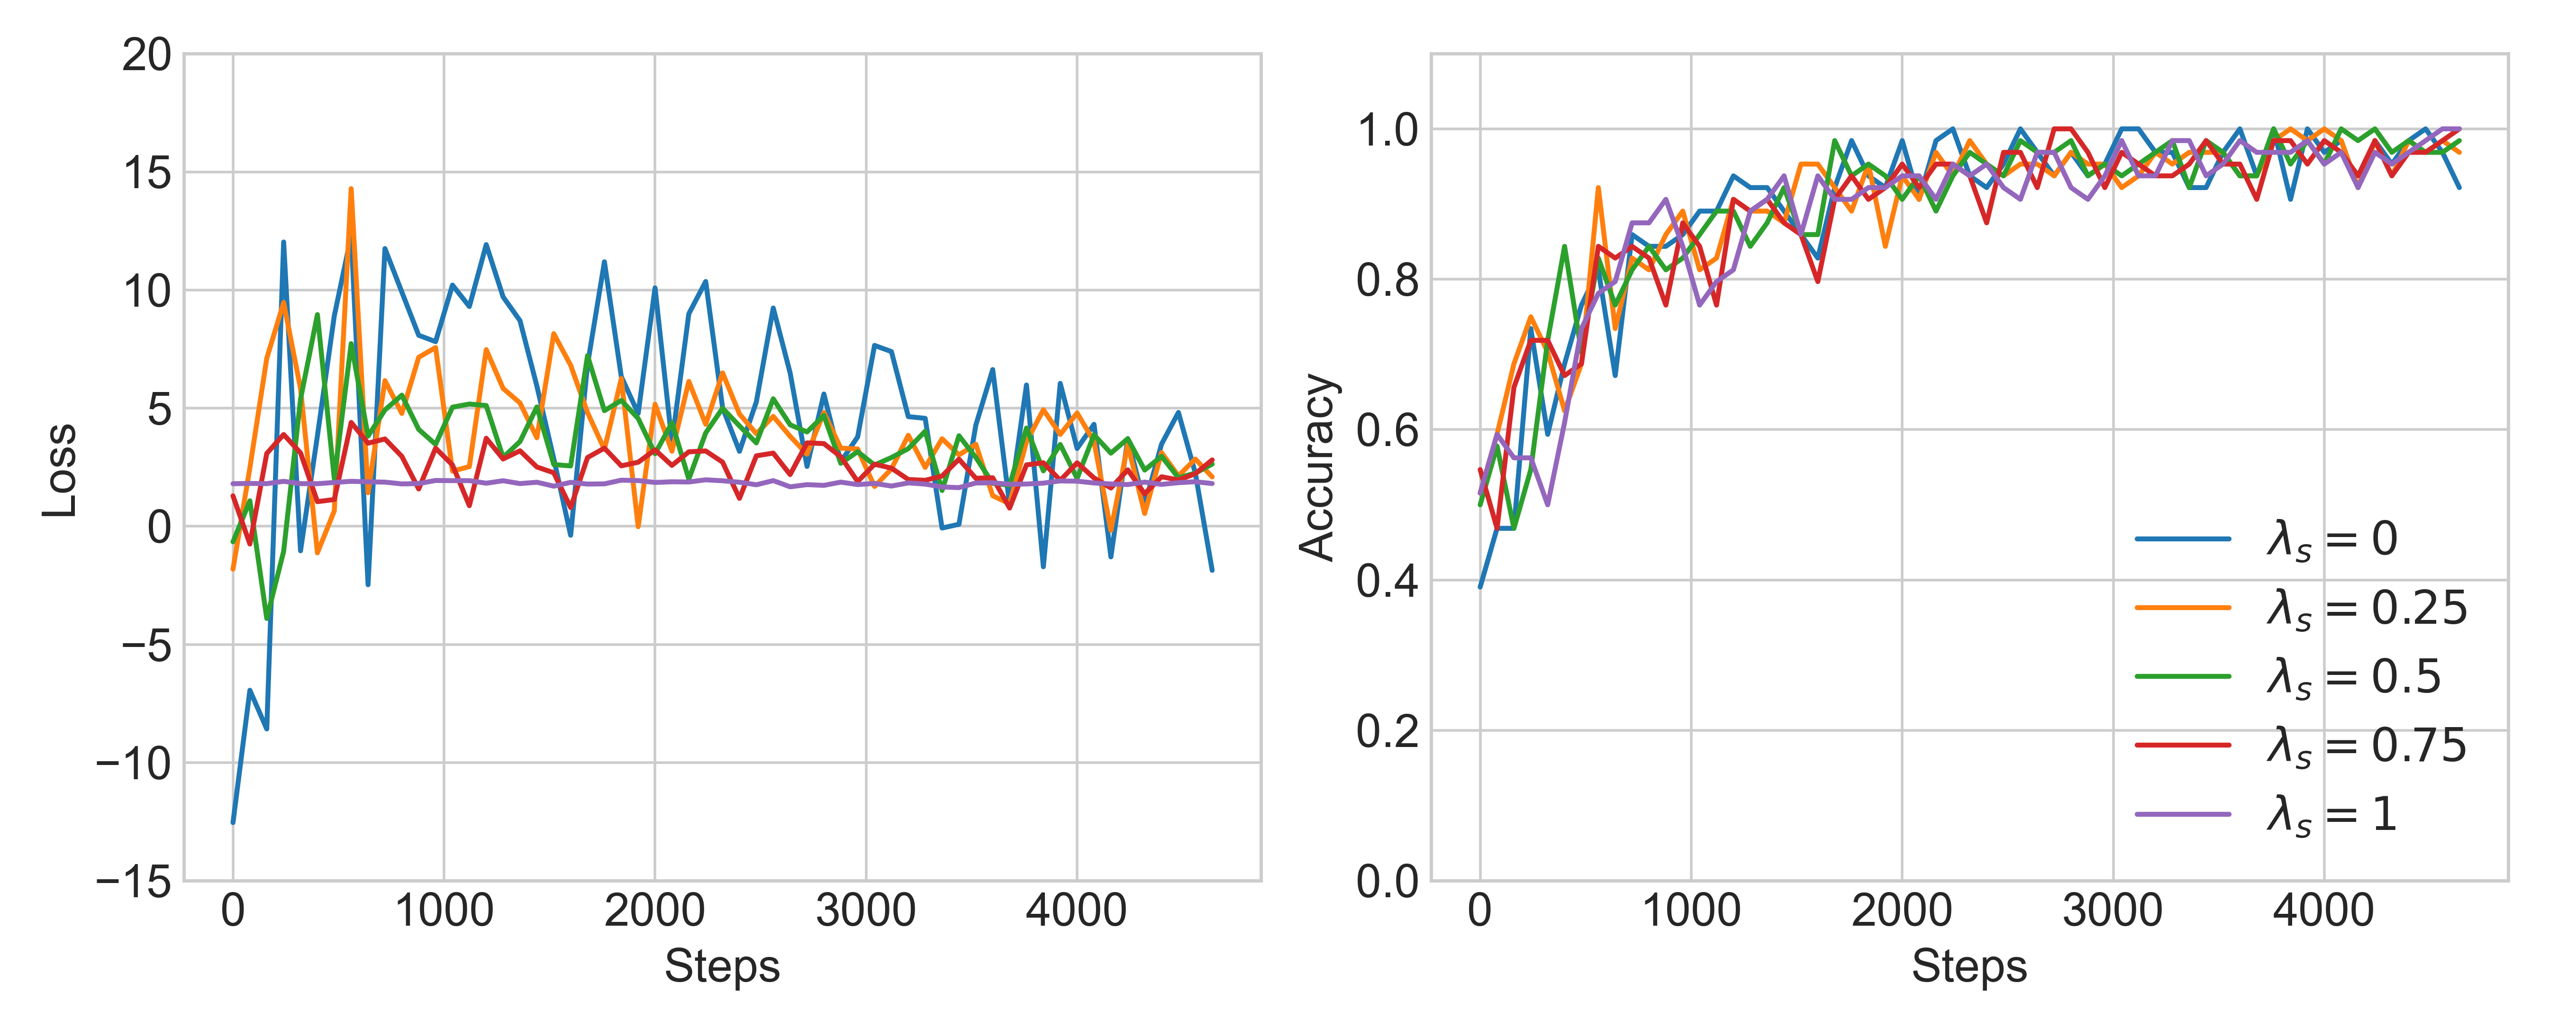
\includegraphics[width=\linewidth]{images/shapes_refgame_49_pure_losses_all_Ls_random.png}
	\caption{Training results of the 3Dshapes experiment with varying $\lambda_s$ weights (pure decoding). Left: Total speaker training loss. Right: Listener training accuracy.}
	\label{fig:3dshapes_baseline_speaker_loss_listener_acc_all}
\end{figure}

\begin{figure}[h]
	\centering
	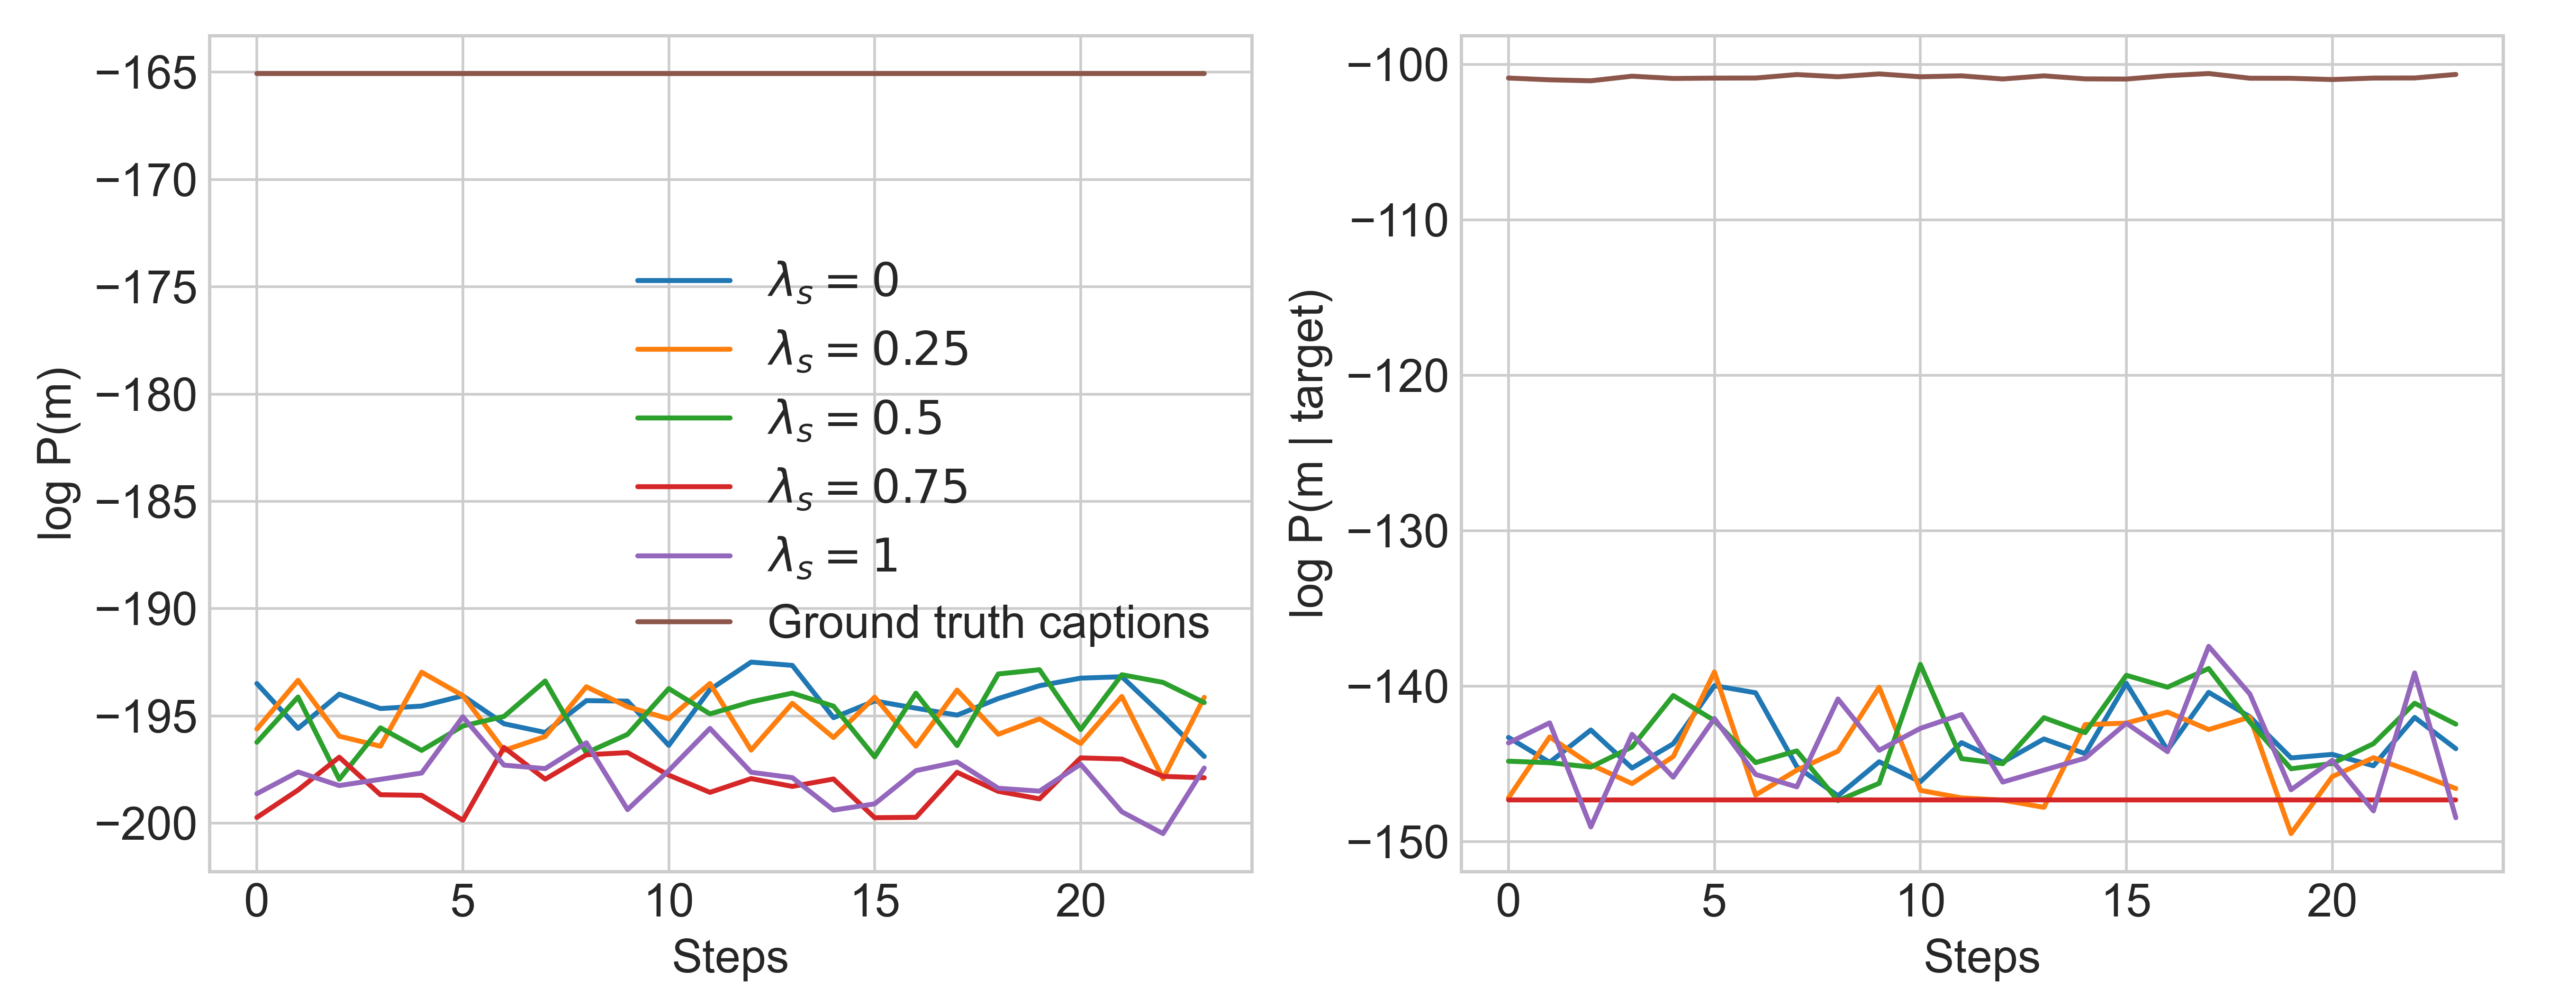
\includegraphics[width=\linewidth]{images/shapes_structural_semantic_drift_49_pure_L_s_all_random.png}
	\caption{Drift metrics computed every 200 training steps on 192 images in the baseline 3Dshapes experiments, across $\lambda_s$ values. Higher values indicate less drift. Left: Strucutral drift of ground truth and predicted captions under a pretrained LM. Right: Semantic drift of ground truth and predicted captions under the pretrained speaker model. The drift is constant for $\lambda_s = 0.75$ due to a coding error, it is the mean validation drift from Table \ref{tab:3dshapes_drift_metrics_basic_baseline}.} 
	\label{fig:3dshapes_baseline_all_str_sem_drift}
\end{figure}

In order to address \textbf{H4} with the 3Dshapes dataset, a line of experiments identical to MS COCO ones was conducted. Specifically, the structural loss weight $\lambda_s$ was also varied. The pattern of results visible in Figure~\ref{fig:3dshapes_baseline_speaker_loss_listener_acc_all} was very similar to MS COCO. The magnitude of the speaker loss is what was mostly influenced by the $\lambda_s$ weight; the listener's training accuracy was not affected by the variation. This is confirmed by the consistently high listener test accuracy, outperforming the pretrained speaker (Table~\ref{tab:3dshapes_drift_metrics_basic_baseline}, fifth column). Differently to MS COCO, the speaker trained with $\lambda_s = 1$ outperformed the pretrained speaker by 0.026, indicating that there might have been room for further pretraining of the speaker. \pt{be careful to not confuse task performance with pretraining; also check this in coco.}

Also following the general procedure, validation language drift metrics on 3Dshapes were computed on a held out test set of 1000 images. Table \ref{tab:3dshapes_drift_metrics_basic_baseline} indicates that, similarly to MS COCO, no clear trends can be observed with respect to all four drift metrics. Negative continuous overlap values (Tab.~\ref{tab:3dshapes_drift_metrics_basic_baseline}, fourth column) indicated that the emebddings of generated captions were partly more similar to the distractor ground truth embeddings, than to target ground truth embeddings. These findings were generally corroborated by the dynamics of structural and semantic drifts computed during training (see Fig.~\ref{fig:3dshapes_baseline_all_str_sem_drift}). In contrast to MS COCO, semantic drift of the captions produced by the speakers was stronger than of the ground truth captions, i.e., the conditional log likelihood of the generated captions was lower. 

These speakers were also evaluated on the image captioning metrics. \pt{TODO Table \ref{tab:eval_metrics_refgame} indicates that the captions for all $\lambda_s$ configurations were closer to ground truth captions compared to MS COCO results.}

These experiments in comparison to analogous experiments on MS COCO (Section \ref{expt:coco_baseline}) also allowed to adress \textbf{H9} as they provided different degrees of freedom for the model to exploit structural deterioration as a method for producing more discrminative captions. In line with \textbf{H9}, the largest difference in structural drift compared to the pretrained speaker in 3Dshapes experiments on random image pairs was 1.058 (Tab.~\ref{tab:3dshapes_drift_metrics_basic_baseline}), compared to 5.164 on MS COCO (Tab.~\ref{tab:coco_drift_metrics_basic}). That is, these results supported \textbf{H9}.

To sum up, similarly to MS COCO, the precise parametrization of the loss did not consistently influence task performance or language drift, given the model and the dataset, indicating that there was no connection to the presence of exhaustive annotation examples in the training dataset.

\subsection{3Dshapes: Similar Pairs Experiments}
\label{expt:3dsapes_similar}

\begin{table}[]
	\begin{tabularx}{\textwidth}{|X|l|l|X|X|X|X|}
		\hline
		\textbf{Model name}                                    & \textbf{log $P(m)$} & \textbf{log $P(m \mid i)$} & \textbf{Overlap (d)} & \textbf{Overlap (c)} & \textbf{Acc. (random)} & \textbf{Acc. (similar)} \\ \hline
		Ground truth exh.       &      -164.752            &         -101.329               &       6.881             &      0.023               &                 &                \\ \hline
		Pretrained 3D exh. speaker                            &       -195.753            &         -145.638               &        5.428              &      0.001                & 0.953 (random listeners)                 & 0.808 (similar listeners)                 \\ \hline
		3D Baseline, random, $\lambda_s = 0.75$  &       -195.495        &           -147.313           &          5.247            &         0.001             & 0.979                                    &                        0.959                   \\ \hline
		3D Baseline, similar, $\lambda_s = 0.75$ &      -198.189             &       -140.786                 &           5.578           &        0.001              & 0.878                      &            0.906                        \\ \hline
		3D Baseline, similar fixed, random test &       -193.709            &    -141.010                  &        3.280            &      -0.003         &            0.688       &                           \\ \hline
		3D Baseline, similar fixed, same test &      -199.014        &        -146.280           &        2.875       &      0.029   &              &          0.691                   \\ \hline
		3D Baseline, similar fixed, diff. test &     -194.510     &    -146.557          &   2.071      & 0.020    &                &              0.570          \\ \hline
		%3D Short, similar, $\lambda_s = 0.75$&      -145.014             &      -76.474                  &             1.565         &         0.000             &                   0.885                       &                                           \\ \hline
		%3D Short, similar fixed, same test $\lambda_s = 0.75$&      -190.010           &     -58.128                  &             2.086         &         0.001             &                   0.731                       &                                           \\ \hline
		%3D Short, similar fixed, diff. test $\lambda_s = 0.75$&     -191.051        &        -59.088           &   1.947        &        0.002          &        0.717                               &                                           \\ \hline
	\end{tabularx}
	\caption{\label{tab:3dshapes_drift_metrics_basic_similar} Language drift metrics and listener test accuracies (``Acc.'') on varying pairs. 
		``Baseline'' refers to the setup wherein the listener is trained jointly with the speaker, using pure decoding. ``Random'' refers to speakers trained on random target-distractor pairs; ``similar'' refers to speakers trained on similar pairs, ``similar fixed'' being the experiments where the image pairs matched on three fixed features. ``Overlap (d)'' refers to the discrete overlap metric, ``overlap (c)'' to continuous overlap. ``Random'' test refers to random held out image pairs, ``same / diff.'' to pairs matching on the same and different features, respectively.}
\end{table}

\begin{figure}[h]
	\centering
	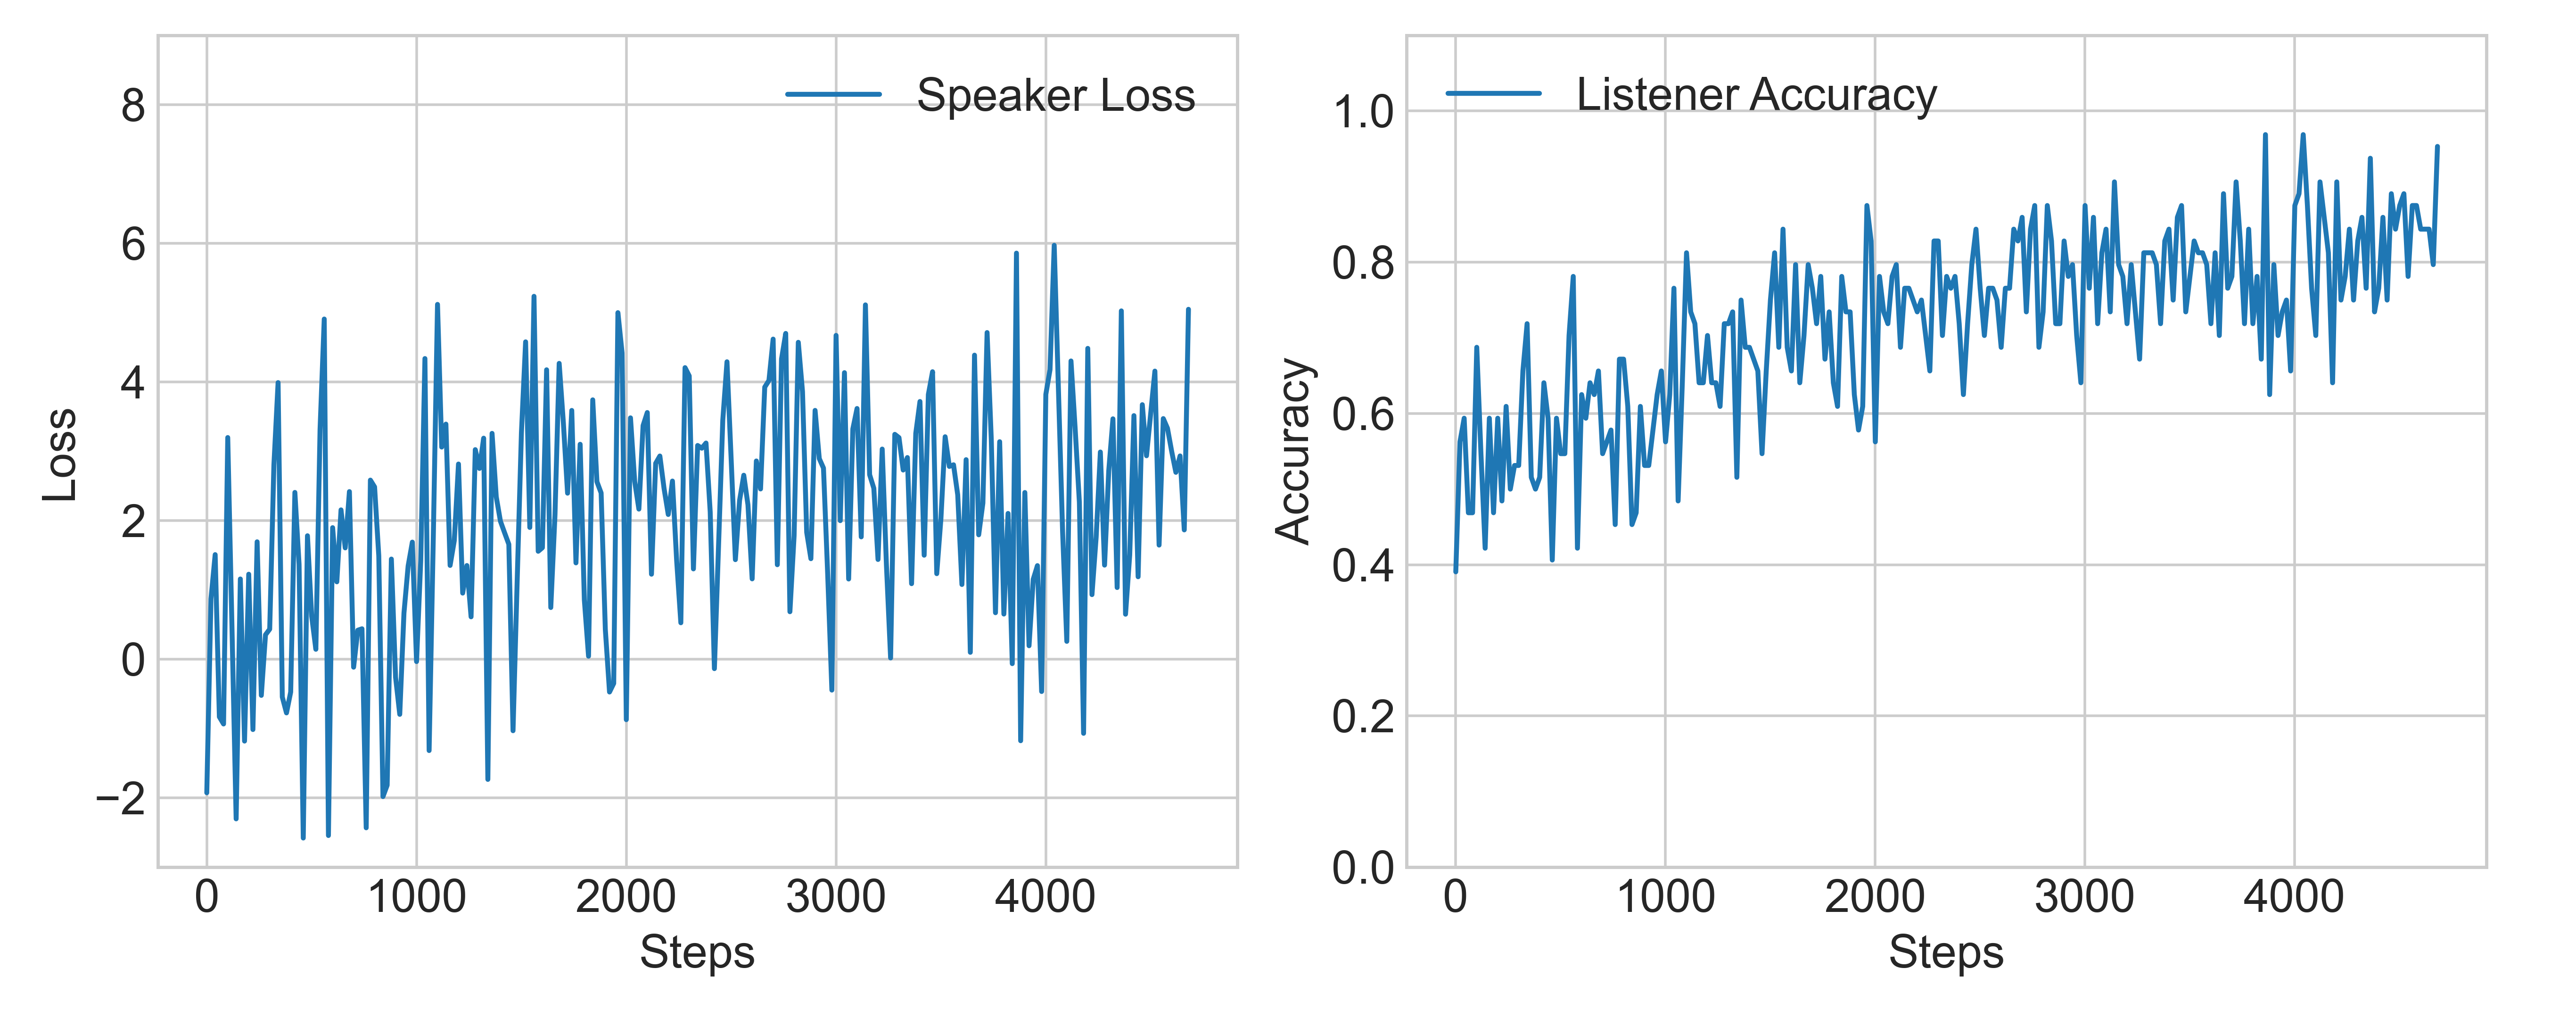
\includegraphics[width=\linewidth]{images/3dshapes_refgame_49_pure_075_similar.png}
	\caption{Training results of the 3Dshapes experiment on similar image pairs (pure decoding, $L_s = 0.75$). Left: Total speaker train loss. Right: Listener train accuracy.}
	\label{fig:3dshapes_similar_075_speaker_loss_listener_acc}
\end{figure}

\begin{figure}[h]
	\centering
	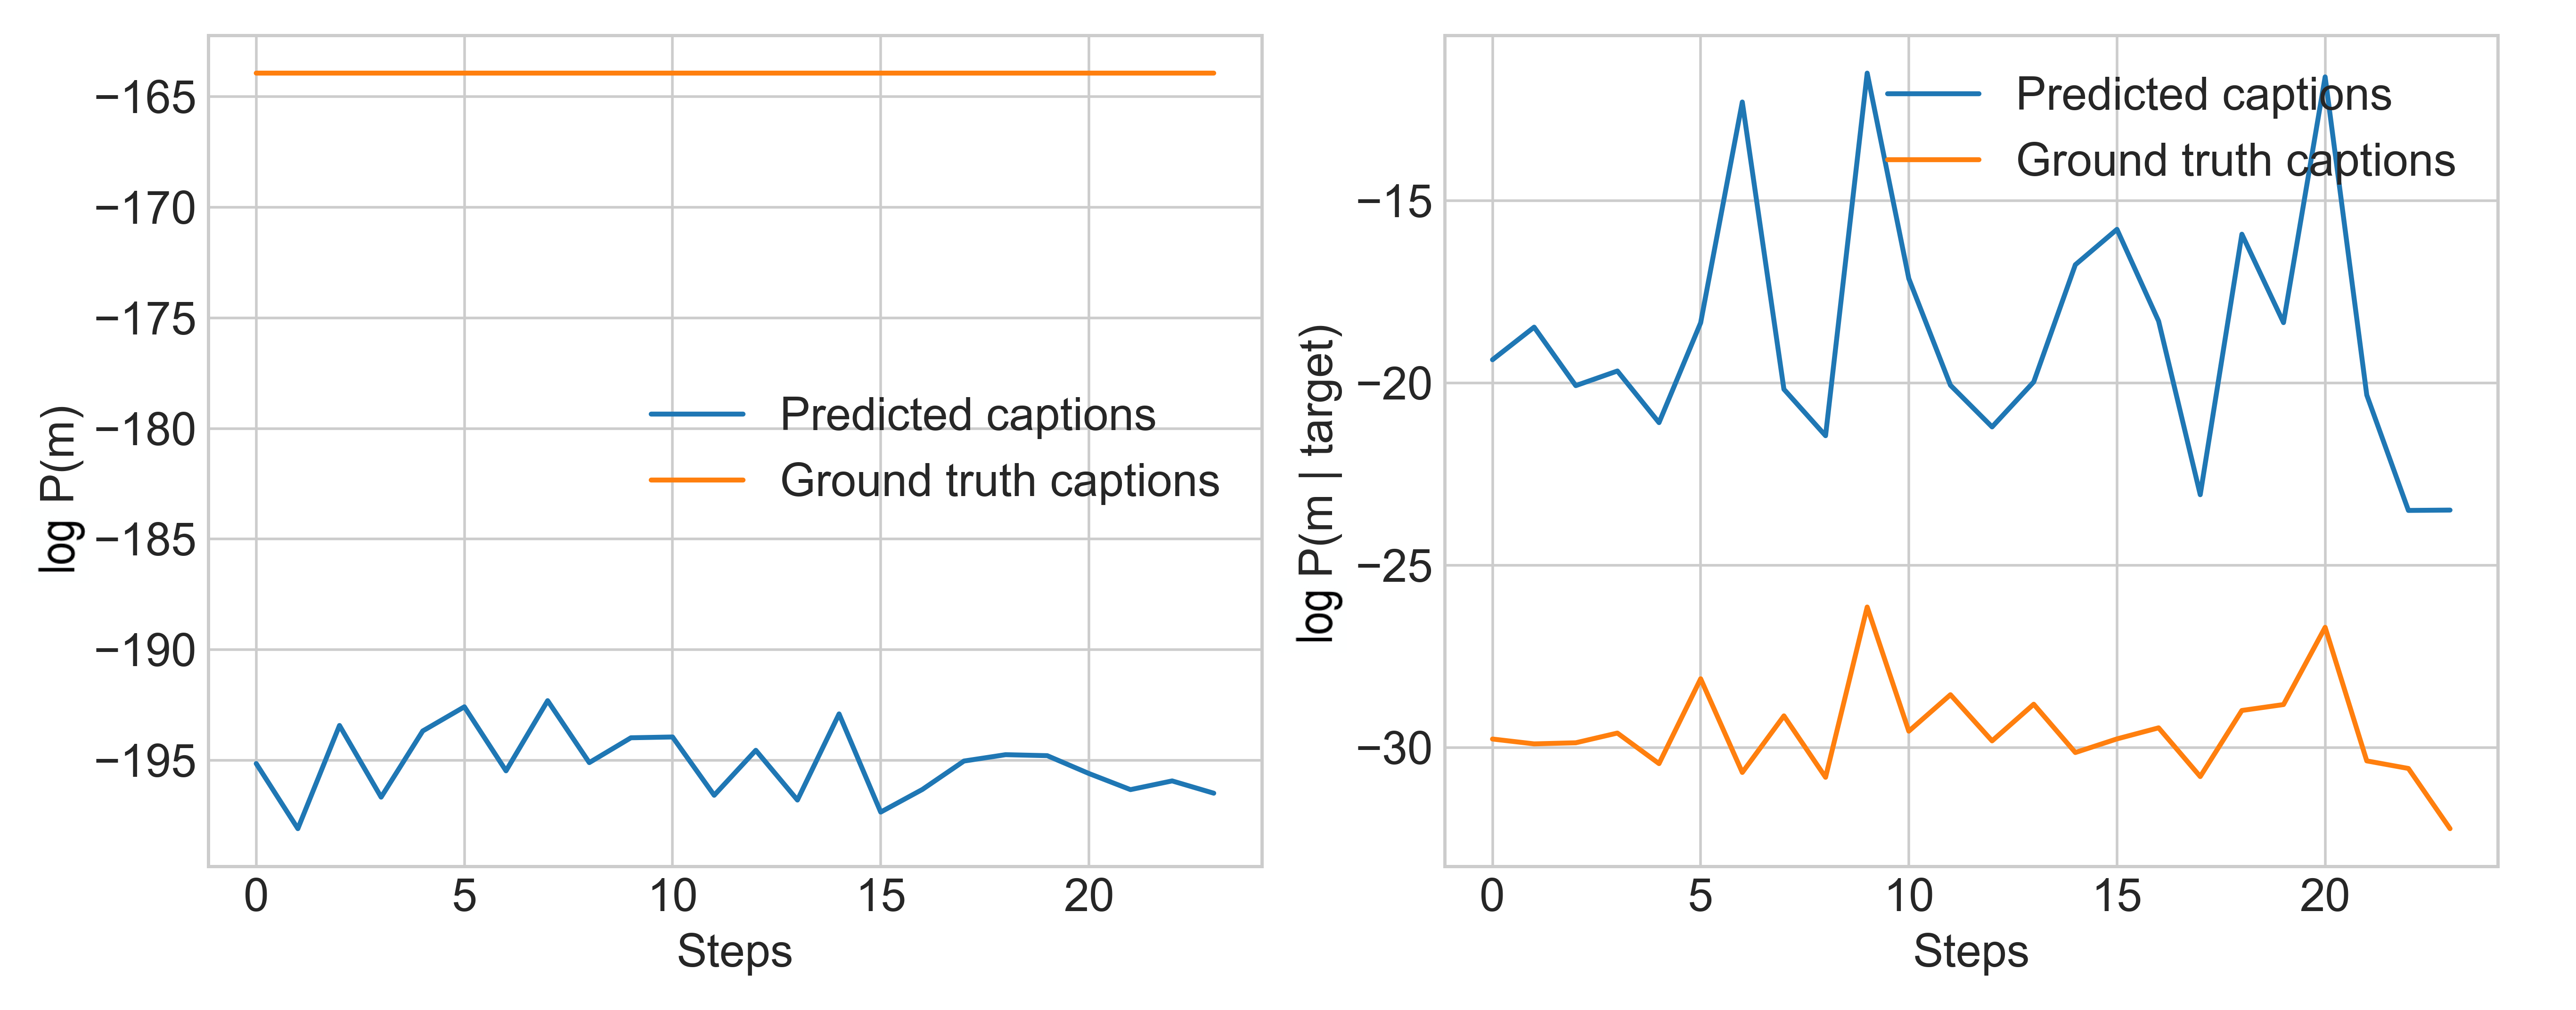
\includegraphics[width=\linewidth]{images/3dshapes_structural_semantic_drift_4000_pure_075_similar.png}
	\caption{Drift values computed during training in the similar image pairs of the 3Dshapes experiment (pure decoding, $L_s = 0.75$, pairs constructed with any features). Higher values are better. Left: Structural drift of ground truth and predicted captions. Right: Semantic drift of ground truth and predicted captions under the model pretrained on similar image pairs.} 
	\label{fig:3dshapes_similar_075_str_sem_drift}
\end{figure}

In this experiment, the target-distractor pairs consisted of similar images. That is, at least three of the six features selected at random matched in the target and distractor image. Otherwise, the procedure and configurations were the same as in the baseline experiment in Section \ref{expt:3dshapes_baseline}. 
Figure \ref{fig:3dshapes_similar_075_speaker_loss_listener_acc} (left) indicates that it was much harder for the speaker to learn producing discriminative messages when the target-distractor pairs were similar, compared to random pairs (Fig.~\ref{fig:3dshapes_baseline_075_speaker_loss_listener_acc}). There were less options for producing discriminative messages, such that the functional training signal was much weaker than in the former experiment. The listener was much slower to learn the reference game and the grounding of the speaker's messages in the images, respectively (Figure \ref{fig:3dshapes_similar_075_speaker_loss_listener_acc}, right). These dynamics confirm that the agents were sensitive to their visual input, and that the task success was closely dependent on the perceptual difficulty to discriminate the target and distractors. These results pattern with the similar pairs experiment on MS COCO (Section \ref{expt:coco_similar_pairs}), although the 3Dshapes agents were faster to learn the reference game on similar pairs. Nonetheless, the agents were still able to learn the reference game successfully, as indicated by rather high test accuracy (Tab.~\ref{tab:3dshapes_drift_metrics_basic_similar}, ``3D Baseline, similar, $\lambda_s = 0.75$'')

The main hypothesis addressed in this experiment was whether the agents were able to flexibly adapt the specificity of their messages, compared to the random pairs baseline experiment (\textbf{H5}). This was approximately investigated via the distribution of POS tags in messaged generated for a test set of 1000 target-distractor pairs.\footnote{The term POS tagging is used in a rather loose sense here---the tags were created manually such that they reflected the specific feature of the image the respective word is used in reference to for this dataset.} The distributions were compared when the 1000 pairs were random versus similar. The results are shown in Figure \ref{fig:3dshapes_pos}. Based on visual inspection, it can be seen that the distribution of the token categories, especially the modifier tokens like color or size adjectives, did not shift significantly depending on the type of pairs (blue~vs.~orange), neither for the random nor the similar pairs experiment speaker. This suggests that the speaker agent was not as flexible in adapting the granularity of feature descriptions in her messages to differences in the input as human speakers (cf. Chapter \ref{chapter03}). Furthermore, there was no apparent difference between speakers trained on the different types of pairs, indicating that the considered training on similar pairs did not lead to better speaker adaptation to more complex visual input. However, it is evident from Figure \ref{fig:3dshapes_similar_075_speaker_loss_listener_acc} that the agents did not converge after two epochs, so longer training might provide a different picture.

\begin{figure}[h]
	\centering
	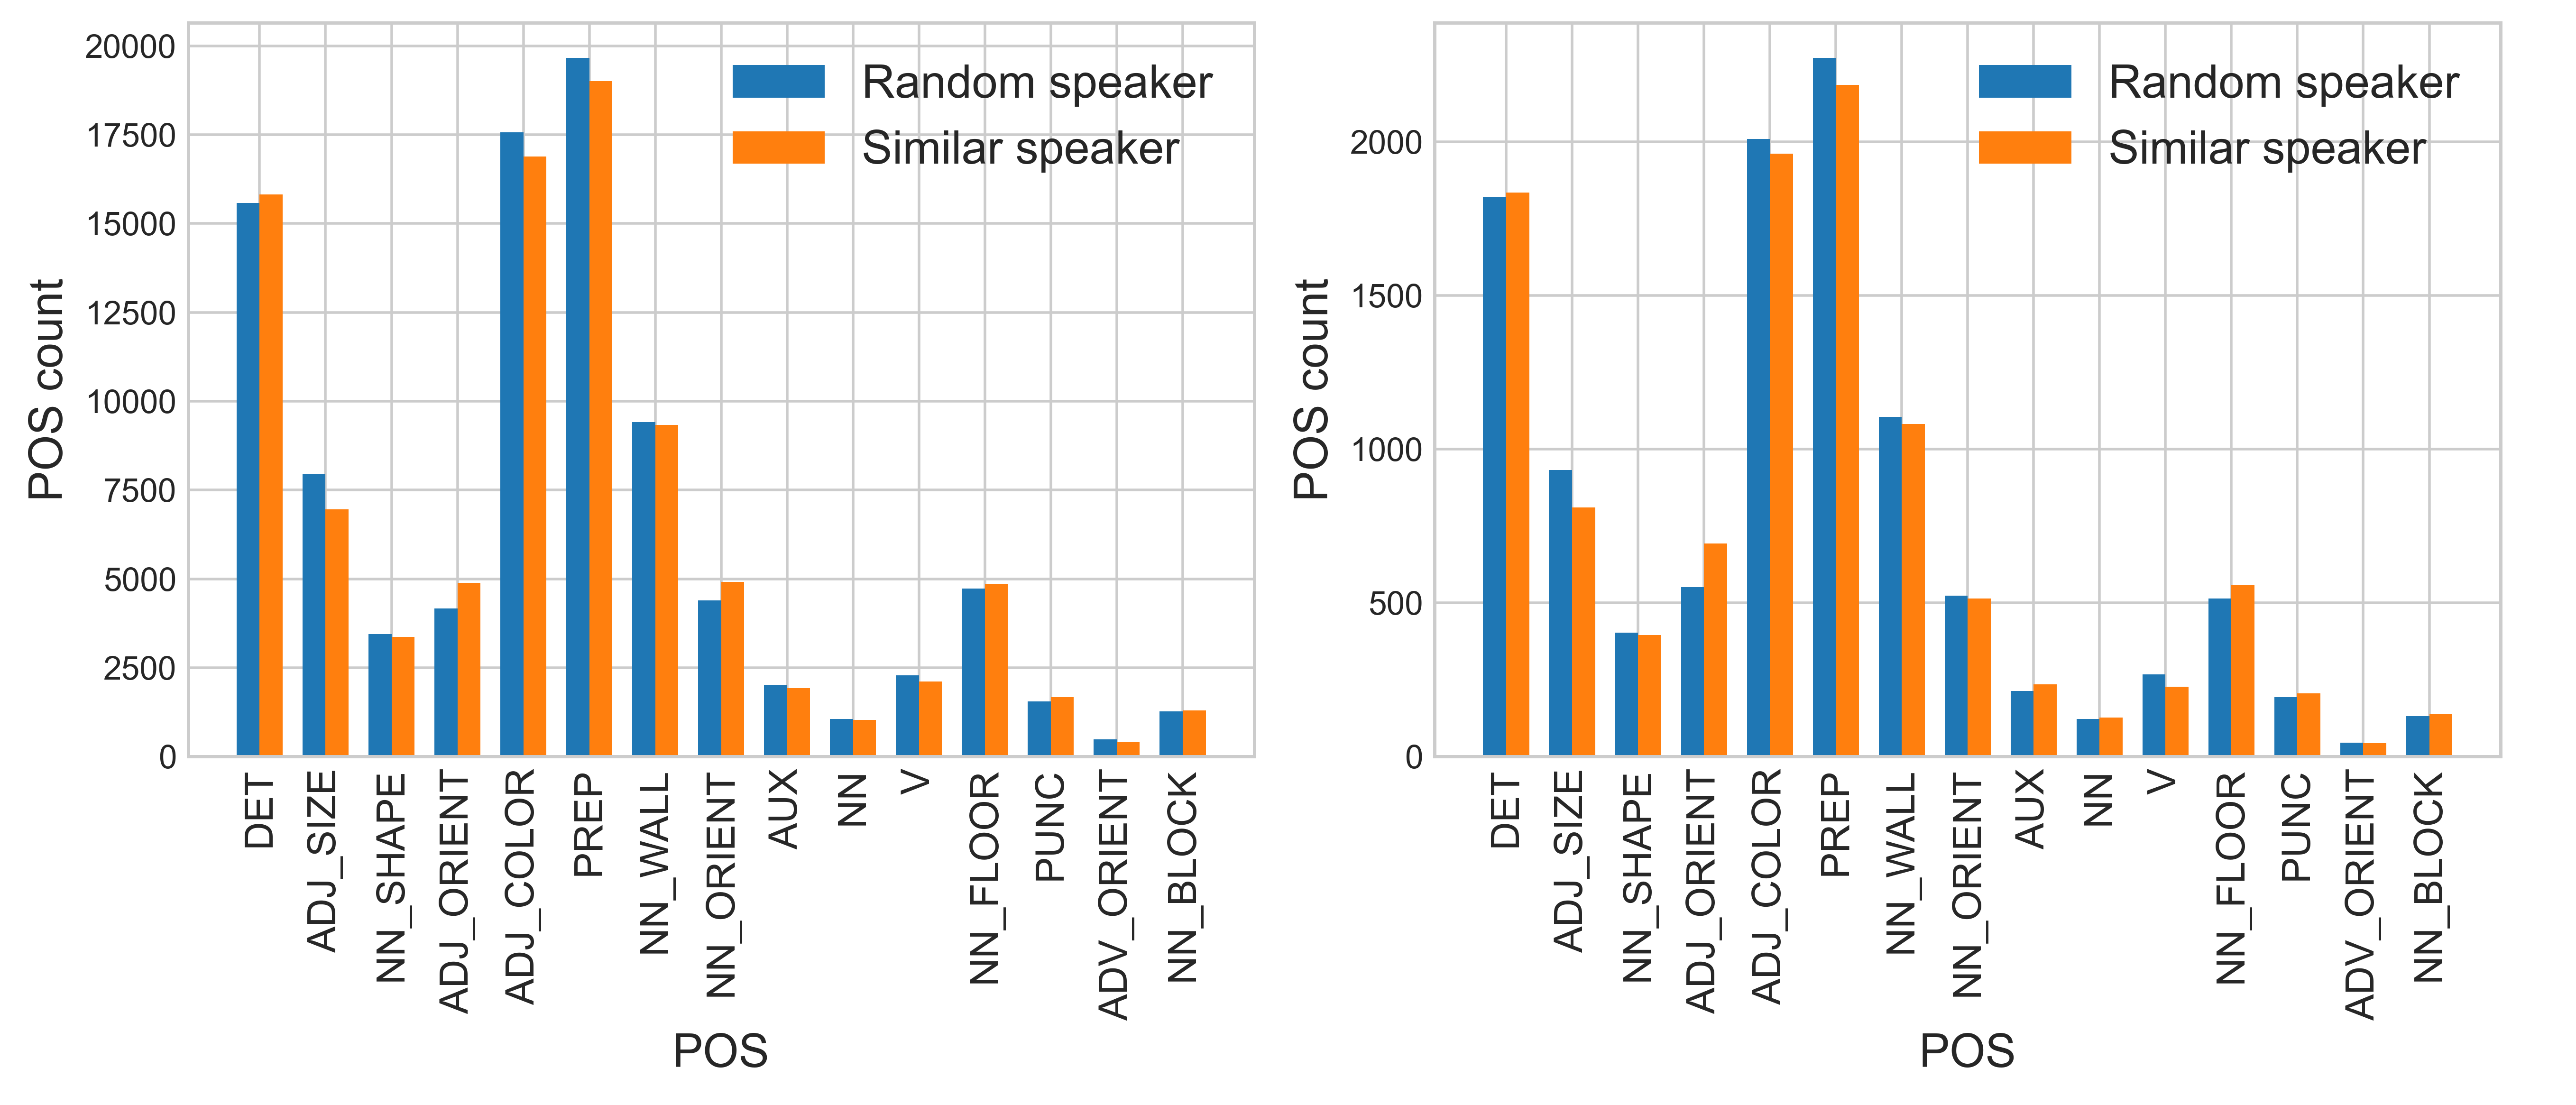
\includegraphics[width=\linewidth]{images/3dshapes_random_vs_similar_POS_counts.png}
	\caption{Left: POS counts in captions produced by a speaker trained on random pairs (blue) and a speaker trained on similar pairs (orange) for 1000 random test image pairs. Right: POS counts in captions produced by a speaker trained on random pairs (blue) and a speaker trained on similar pairs (orange) for 100 similar test image pairs. \pt{The difference in the number of pairs will be fixed}}
	\label{fig:3dshapes_pos}
\end{figure}

In this experiment, stronger structural drift compared to both the pretrained speaker and the baseline experiment could be observed (see Table \ref{tab:3dshapes_drift_metrics_basic_similar}), which was corroborated by a slight visually apparent trend in Figure \ref{fig:3dshapes_similar_075_str_sem_drift}.\footnote{The same coding mistake also led to the use of 50 images from the training dataset and greedy decoding for semantic drift during the training drift computations.} Again patterning with MS COCO results, semantic drift was lower for the similar pairs compared to the random pairs experiment. Going beyond MS COCO, the drift was even smaller than for the pretrained speaker (Tab.~\ref{tab:3dshapes_drift_metrics_basic_similar}). This suggests that the reference game signal helped fine-tuning the speaker.
A little increase in the discrete overlap compared to the pretrained speaker and to the random pairs baseline indicated that the speaker improved on the task and found a way of producing slightly more discriminative messages (Tab.~\ref{tab:3dshapes_drift_metrics_basic_similar}), inspite of perceptual similarity of the images. In sum, these similar pairs experiment results on 3Dshapes did not provide evidence in support of \textbf{H5}. One reason for this might be the variability in the features the images matched on and the potentially varying difficulty for a model to discriminate them. For instance, fine-grained object size differences might be more difficult to detect compated to different object types.

So in order to investigate effects of visual pair similarity in more detail, a follow-up experiment was conducted wherein the features along which the target and the distractor matched were fixed. These features were the object type (cube, ball, pill or cylinder), the object color and the background color. For instance, assuming that the first image on the left in Fig.~\ref{fig:3dshapes_example} was the target, the distractor could depict a cyan smaller cube in front of the same blue wall, but in the left corner and on red floor.
The selection of these features for being fixed was rather arbitrary, and follow-up experiments should address the visual discriminability of different features more systematically. The training results can be seen in Figure~\ref{fig:3dshapes_wShort_similarFixed_075_speaker_losses_listener_acc} (blue lines). Visually, the agents' task performance did not differ much from the random pairs experiments (Fig. \ref{fig:3dshapes_baseline_075_speaker_loss_listener_acc}). Yet compared to the previous experiment wherein all fixed features were considered, the agents learned the reference game more quickly (Fig.~\ref{fig:3dshapes_similar_075_speaker_loss_listener_acc}). In order to investigate the listener's test accuracy as well as details of language drift, two kinds of evaluations were done. First, the agents were tested on a held out test set of 1000 similar image pairs which matched along the same features as the pairs used during training (`same features' test). Second, they were tested on a held out test set of 1000 image pairs which matched along the \emph{other three} features than the training pairs (i.e., floor color, size of the object and its position in the room, `different features' test). The motivation for this distinction was to investigate whether the speaker was capable to adjust the granularity of her messages depending on the familiarity of the distinctive features.

The listener test accuracy of 0.691 (Table \ref{tab:3dshapes_drift_metrics_basic_short}) on the same features test set was surprisingly low compared to the training accuracy (Fig. \ref{fig:3dshapes_wShort_similarFixed_075_speaker_losses_listener_acc}, right, blue line), hinting at potential speaker-listener co-adaptation and overfitting on the training set. The test accuracy on different features was even lower (0.570), confirming that it was more difficult for the agents to communicate about unfamiliar distinctive features. 

The language drift dynamics shown in Figure \ref{fig:3dshapes_wShort_similarFixed_075_str_sem_drift} (blue and green lines) were similar to the random pairs experiments dynamics. While this patterned with MS COCO results regarding structural drift (see Section \ref{expt:coco_similar_pairs}), in contrast to MS COCO, there was no increase in semantic drift during training here. This indicates that the 3Dshapes agents did not resort to speaker-listener co-adaptation as strongly, possibly due to higher tractability of the action space and easier grounding of the listener, even in context of similar image pairs.
Table \ref{tab:3dshapes_drift_metrics_basic_short} shows that structural drift increased for the same features test compared to both the random pairs baseline and the pretrained speaker. Interestingly, it was not the case for semantic drift which even slightly improved compated to the random pairs baseline. These results suggest that the speaker did not resort to drift behavior as a functional improvement strategy given more complex context. The discrete overlap decreased compared to the random baseline for both tests (and even more so for the same features test), mirroring the increased difficulty to select words that apply to the target but not to the distractor. Further, this experiment was the first one showing a significant increase in continuous overlap compared to both pretrained speaker and random baseline; therefore, perhaps the fine-grained functional signal was advantageuous for shaping the embedding space of the speaker more precisely. Finally, addressing the question of speaker flexibility with increasing pressure towards more granular messages, in Figure \ref{fig:3dshapes_exh_short_same_diff_lengths} (right), a tendency towards longer messages for the different features test set could be observed. That is, the speaker might flexibly adjust her message granularity as approximated by message length to contextual needs. % and, to some extend, listener expectations (as represented by the implicit adaptation to the listener which was trained jointly with the speaker on other feature pairs). 
Analysing the distribution of POS tags in the different test sets (akin to the analysis described above), it can be observed in Figure~\ref{fig:3dshapes_exh_short_same_diff_POS} (left) that, although, visually, the differences in the occurrence frequencies were marginal, some intuitions were borne out. Intuitively, the discriminative features for the same features test set were the color of the floor, the orientation and the size of the object. For the different features test set, these were the color of the background (i.e., wall), the object's color and its type.
Indeed, the speaker referred to the floor (``NN\_FLOOR'' tag) and the orientation of the object (``ADJ\_ORIENT'', ``ADV\_ORIENT'') more frequently for the same test set than for the different test set. This was not the case for the size of the object (``ADJ\_SIZE''). For the different features test set, she referred to the wall (``NN\_WALL'') and the object type (``NN\_SHAPE'') more frequently. 
The distribution of color references would require a more detailed analysis in order to disentangle which part of the image it might apply to. That is, these results indicate that the speaker was capable of identifying discriminative features of the images. Given that there was almost no difference in this capacity between the two test sets (same~vs.~different features), one could hypothesize that this flexibility was driven by the skills from pretraining rather than reference game based adaptation. However, tests with splits along other features fixed during reference game training would provide a more comprehensize picture.

To sum up, this follow-up experiment further supported \textbf{H5} on the 3Dshapes dataset, at least in terms of discrete overlap and with respect to speaker's message flexibility.

%\pt{Add results to table, finish discussion, compare convergence speed to randomly chosen similar pairs, overall random pairs experiment}

\subsection{3Dshapes: Fixed Listener Experiments}
\label{expt:3dshapes_fixed}

Similarly to MS COCO in Section \ref{exp:coco_fixed_listener}, \textbf{H6} was also investigated for the 3Dshapes dataset in an analogous set up. The fixed listener was pretrained on exhaustive captions, and showed a post-pretraining test accuracy of 0.998 on ground truth held out test captions and 0.920 with the pretrained speaker messages on the same held out test set. 

The results on 3Dshapes patterned with those on MS COCO both in terms of training dynamics (Fig.~\ref{fig:3dshapes_fixed_listener_0_075_speaker_losses_listener_acc}, orange line) and the listener test accuracy being lower than for the joint listener experiment and the pretrained speaker (Tab.~\ref{tab:3dshapes_drift_metrics_basic_baseline}). That is, given the test accuracy of 0.927, no strong improvement beyond the listener's pretraining accuracy was observed. 
The lower accuracy compared to the pretrained speaker could be attributed to the fact that the listener was pretrained on ground truth captions and then tested with speaker generated captions which were somewhat different from the ground truth due to the auto-regressive generation (see Appendix \ref{app:grid_search}). 
\begin{figure}[h]
	\centering
	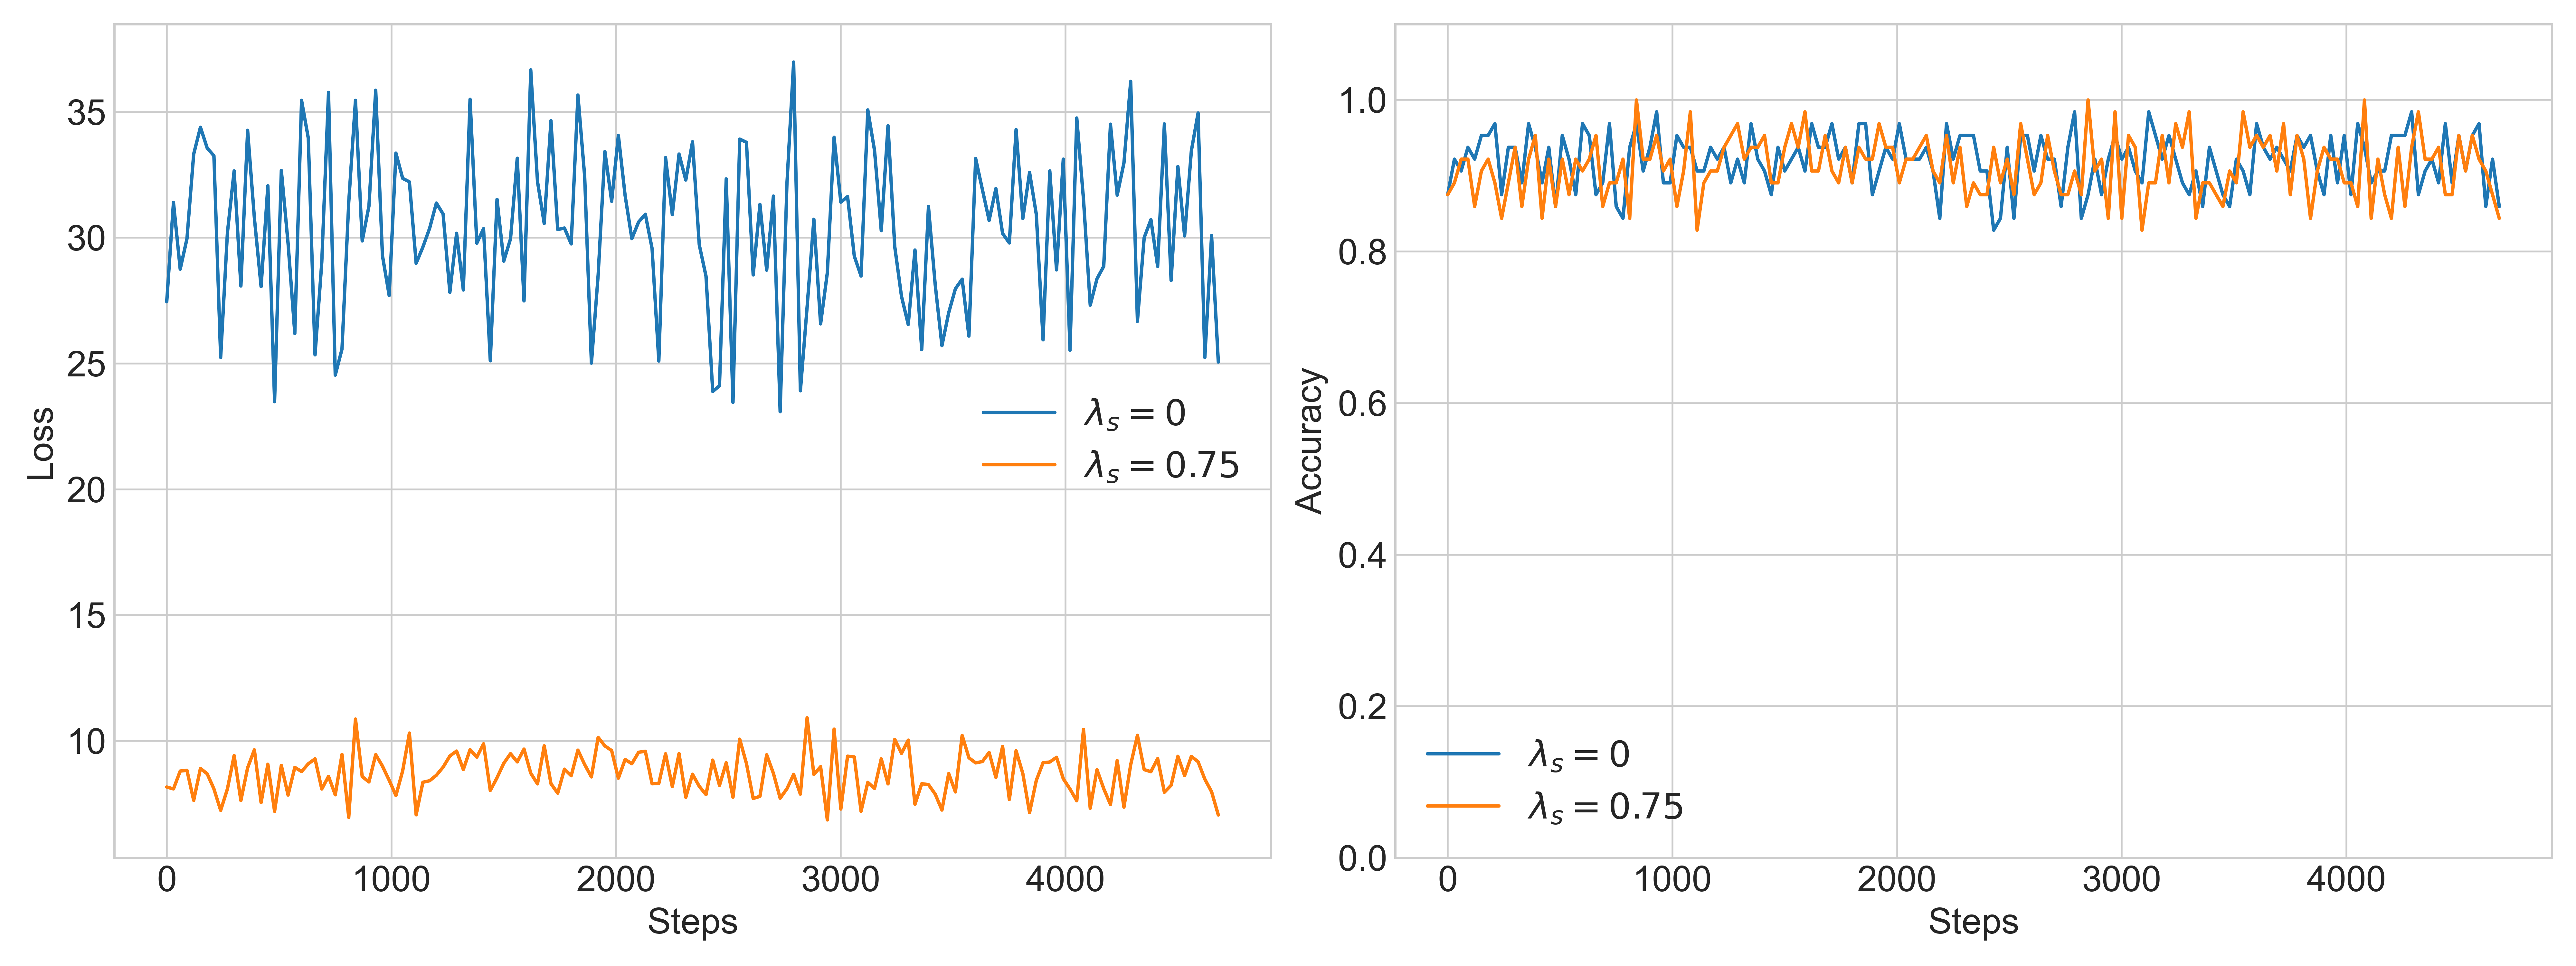
\includegraphics[width=\linewidth]{images/3dshapes_fixedListener_baseline_random_0_075_losses.png}
	\caption{Training results of reference games against a fixed listener on exhaustive captions of 3Dshapes (pure decoding, $\lambda_s=0$ vs. $\lambda_s=0.75$). Left: Total speaker training loss. Right: Listener training accuracy.}
	\label{fig:3dshapes_fixed_listener_0_075_speaker_losses_listener_acc}
\end{figure}

Similarly to MS COCO, training the speaker against a fixed listener also mitigated both structural and semantic drift (Tab.~\ref{tab:3dshapes_drift_metrics_basic_baseline}). In fact, the drift decreased even compared to the pretrained speaker. This suggests that in a smaller action space of the 3Dshapes experiment, the functional training signal from the listener pretrained on ground truth captions might be strong enough to further fine-tune the speaker towards more ground truth-like messages. However, the signal appeared to not be strong enough in order to lead to definitive increases in the overlap metrics, compared to the pretrained speaker (Tab. \ref{tab:3dshapes_drift_metrics_basic_baseline}). 

\pt{TODO image caption evaluation}
\begin{figure}[h]
	\centering
	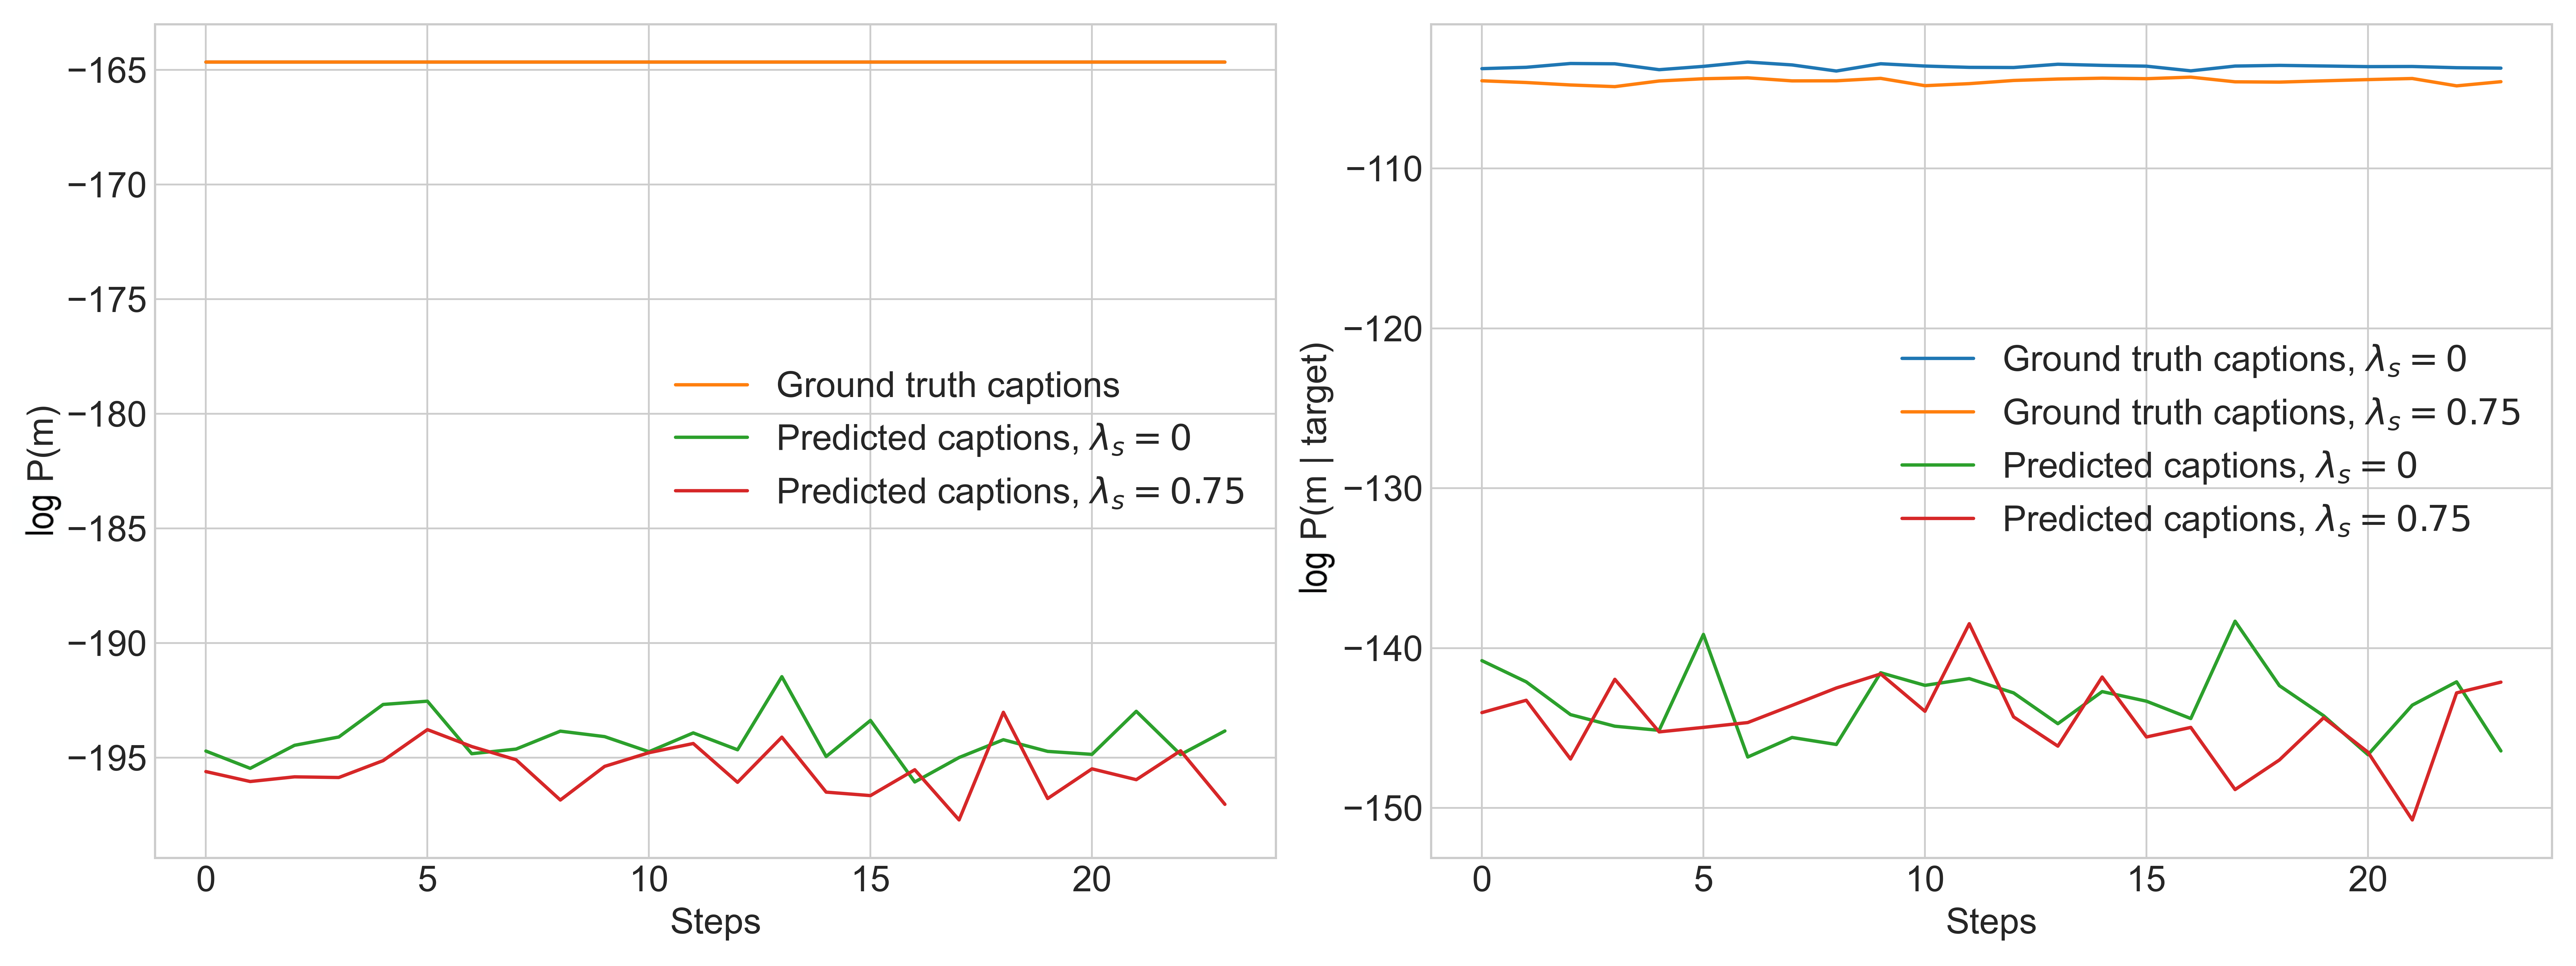
\includegraphics[width=\linewidth]{images/3dshapes_fixedListener_structural_semantic_drift_49_pure_0_075_random.png}
	\caption{Drift dynamics computed during reference game training with the fixed listener on 3Dshapes (pure decoding, $\lambda_s=0$ vs. $\lambda_s=0.75$). Higher values indicate less drift. Left: Structural drift of ground truth and predicted captions under the pretrained LM. Right: Semantic drift of ground truth and predicted captions under the pretrained speaker model.}
	\label{fig:3dshapes_fixed_listener_0_075_str_sem_drift}
\end{figure}

In order to investigate whether it was indeed the functional task signal that was responsible for mitigating the language drift, and whether better task improvement can be achieved given a stronger functional signal, a follow-up experiment with a functional loss only (i.e., $\lambda_s=0$) was also conducted for 3Dshapes. While the task success was not visibly improved (see Fig.~\ref{fig:3dshapes_fixed_listener_0_075_speaker_losses_listener_acc}, right, orange vs. blue line), structural and semantic drifts during training were indeed slightly lower for $\lambda_s=0$, compared to $\lambda_s=0.75$ (Fig.~\ref{fig:3dshapes_fixed_listener_0_075_str_sem_drift}, green line being slightly above the red one).\footnote{Semantic drift values of the ground truth are slightly different due to the known non-deterministic behaviour of some CUDA supporting RNN implementations in Pytorch, even with a random seed.} Validation results in Table \ref{tab:3dshapes_drift_metrics_basic_baseline} indicate that semantic drift was better mitigated under a stronger functional training signal ($\lambda_s =0$ compared to $\lambda_s =0.75$), suggesting that the grounding was better preserved. Structural drift, however, increased, compared to $\lambda_s =0.75$, which is expected given that there was no structural learning signal anymore in the $\lambda_s =0$ experiment. Further confirming intuitions regarding the role of the functional learning signal, the discrete overlap increased in the $\lambda_s =0$ configuration, outperforming the baseline joint listener experiment. The continuous overlap, on the other hand, decreased, compared to both pretrained and baseline joint speakers, indicating that the functional improvements might not be translated to topographic effects in the embedding space \parencite[cf.][]{lazaridou2018emergence}. Overall, results with both $\lambda_s$ configurations supported \textbf{H6}.

Additionally, in order to address the apparent overfitting and co-adaptation of the joint speaker and listener in the previous similar pairs experiment (Section~\ref{expt:3dsapes_similar}), as was apparent from the discrepancy between the training and testing accuracies (Fig.~\ref{fig:3dshapes_wShort_similarFixed_075_speaker_losses_listener_acc}, blue lines, and Tab.~\ref{tab:3dshapes_drift_metrics_basic_similar}), a follow-up experiment with a fixed listener was conducted. It also used similar pairs matching on the three fixed categories, and exhaustive captions. 
The training dynamics in Figure~\ref{fig:3dshapes_similarFixed_fixedListener_075_speaker_loss_listener_acc} were similar to the training on random pairs (cf.~Fig.~\ref{fig:3dshapes_fixed_listener_0_075_speaker_losses_listener_acc}), and resulted in a lower training accuracy than with the joint listener. The test accuracies both on the same features and different features test sets were closer to the training accuracy (Tab.~\ref{tab:3dshapes_drift_metrics_basic_baseline}, last two lines), showing that the discrepancy between trainining and test accuracy in Section \ref{expt:3dsapes_similar} was at least to some extend due to speaker-listener co-adaptation on the trianing dataset. At the same time, the listener's accuracy did not improve beyond pretraining level (it was, in fact, worse than the pretraining test accuracy on random pairs), indicating that the speaker did not adapt her messages to functional needs much. Surprisingly, the test accuracy was higher on the different features test set than on the same features set. This could be attributed to potential differences in the listener's ability to discriminate the particular features belonging to either set, as induced by the pretraining. Compared to the accuracy difference between the test sets in the joint listener experiment, it can also be inferred that reference game fine-tuning for two epochs was not sufficient for overriding the agents' capabilities learned during pretraining in the fixed listener experiment, like communicating about features which were not part of the reference game training but were used in the pretraining.

Visually, the drift dynamics during training also did not differ between the fixed and the joint listener experiments (Fig.~\ref{fig:3dshapes_similarFixed_fixedListener_075_str_sem_drift}~vs.~Fig.~\ref{fig:3dshapes_wShort_similarFixed_075_str_sem_drift}, blue and green lines). Interestingly, in contrast to random pairs, the semantic drift values did not improve with the fixed listener compared to the joint listener on the same features test set, but did improve on the different features test set (Tab.~\ref{tab:3dshapes_drift_metrics_basic_baseline}~vs.~Tab.~\ref{tab:3dshapes_drift_metrics_basic_similar}). The results were the other way around for structural drift. The discrete overlap was higher for both tests for the fixed listener than the joint one, and so was the continuous overlap on the different features test set.
Taken together, these results indicate that given more complex visual input, the listener grounding was more susceptible to overfitting, yet the functional signal was not strong enough so as to result in speaker-listener co-adaptation measured by semantic drift. Therefore, it seems to be a difficult task to fine-tune the speaker for a task on complex visual input in a way that provides a sufficiently strong task success signal, while also achieving a good generalization performance. 

\begin{figure}[h]
	\centering
	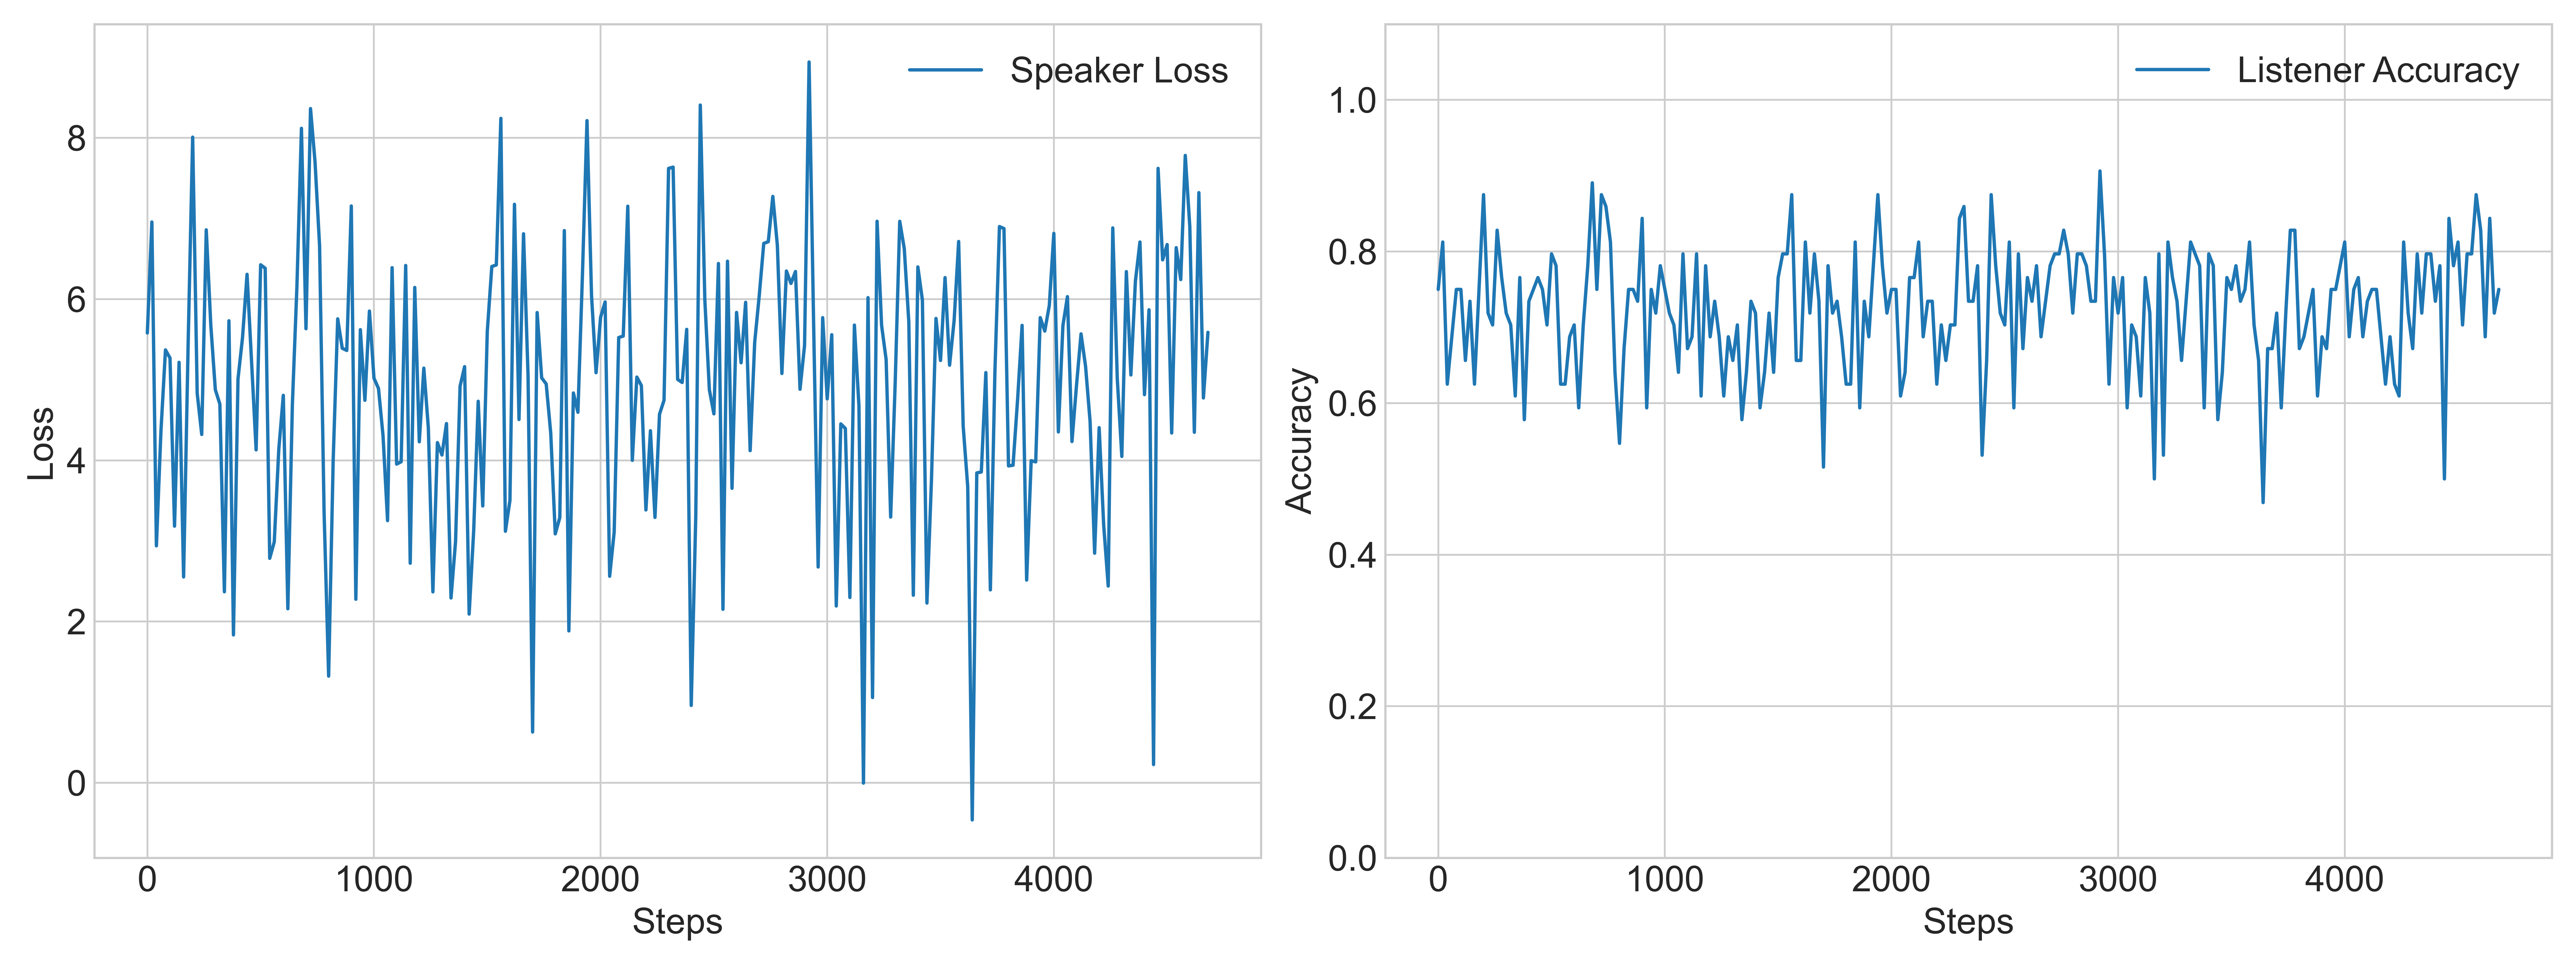
\includegraphics[width=\linewidth]{images/3dshapes_fixedListener_similarFixed_exh_075_losses.png}
	\caption{Training results of the 3Dshapes experiment on similar image pairs with fixed matching features with a fixed listener (pure decoding, exhaustive captions, $L_s = 0.75$). Left: Total speaker training loss. Right: Listener training accuracy.}
	\label{fig:3dshapes_similarFixed_fixedListener_075_speaker_loss_listener_acc}
\end{figure}

\begin{figure}[h]
	\centering
	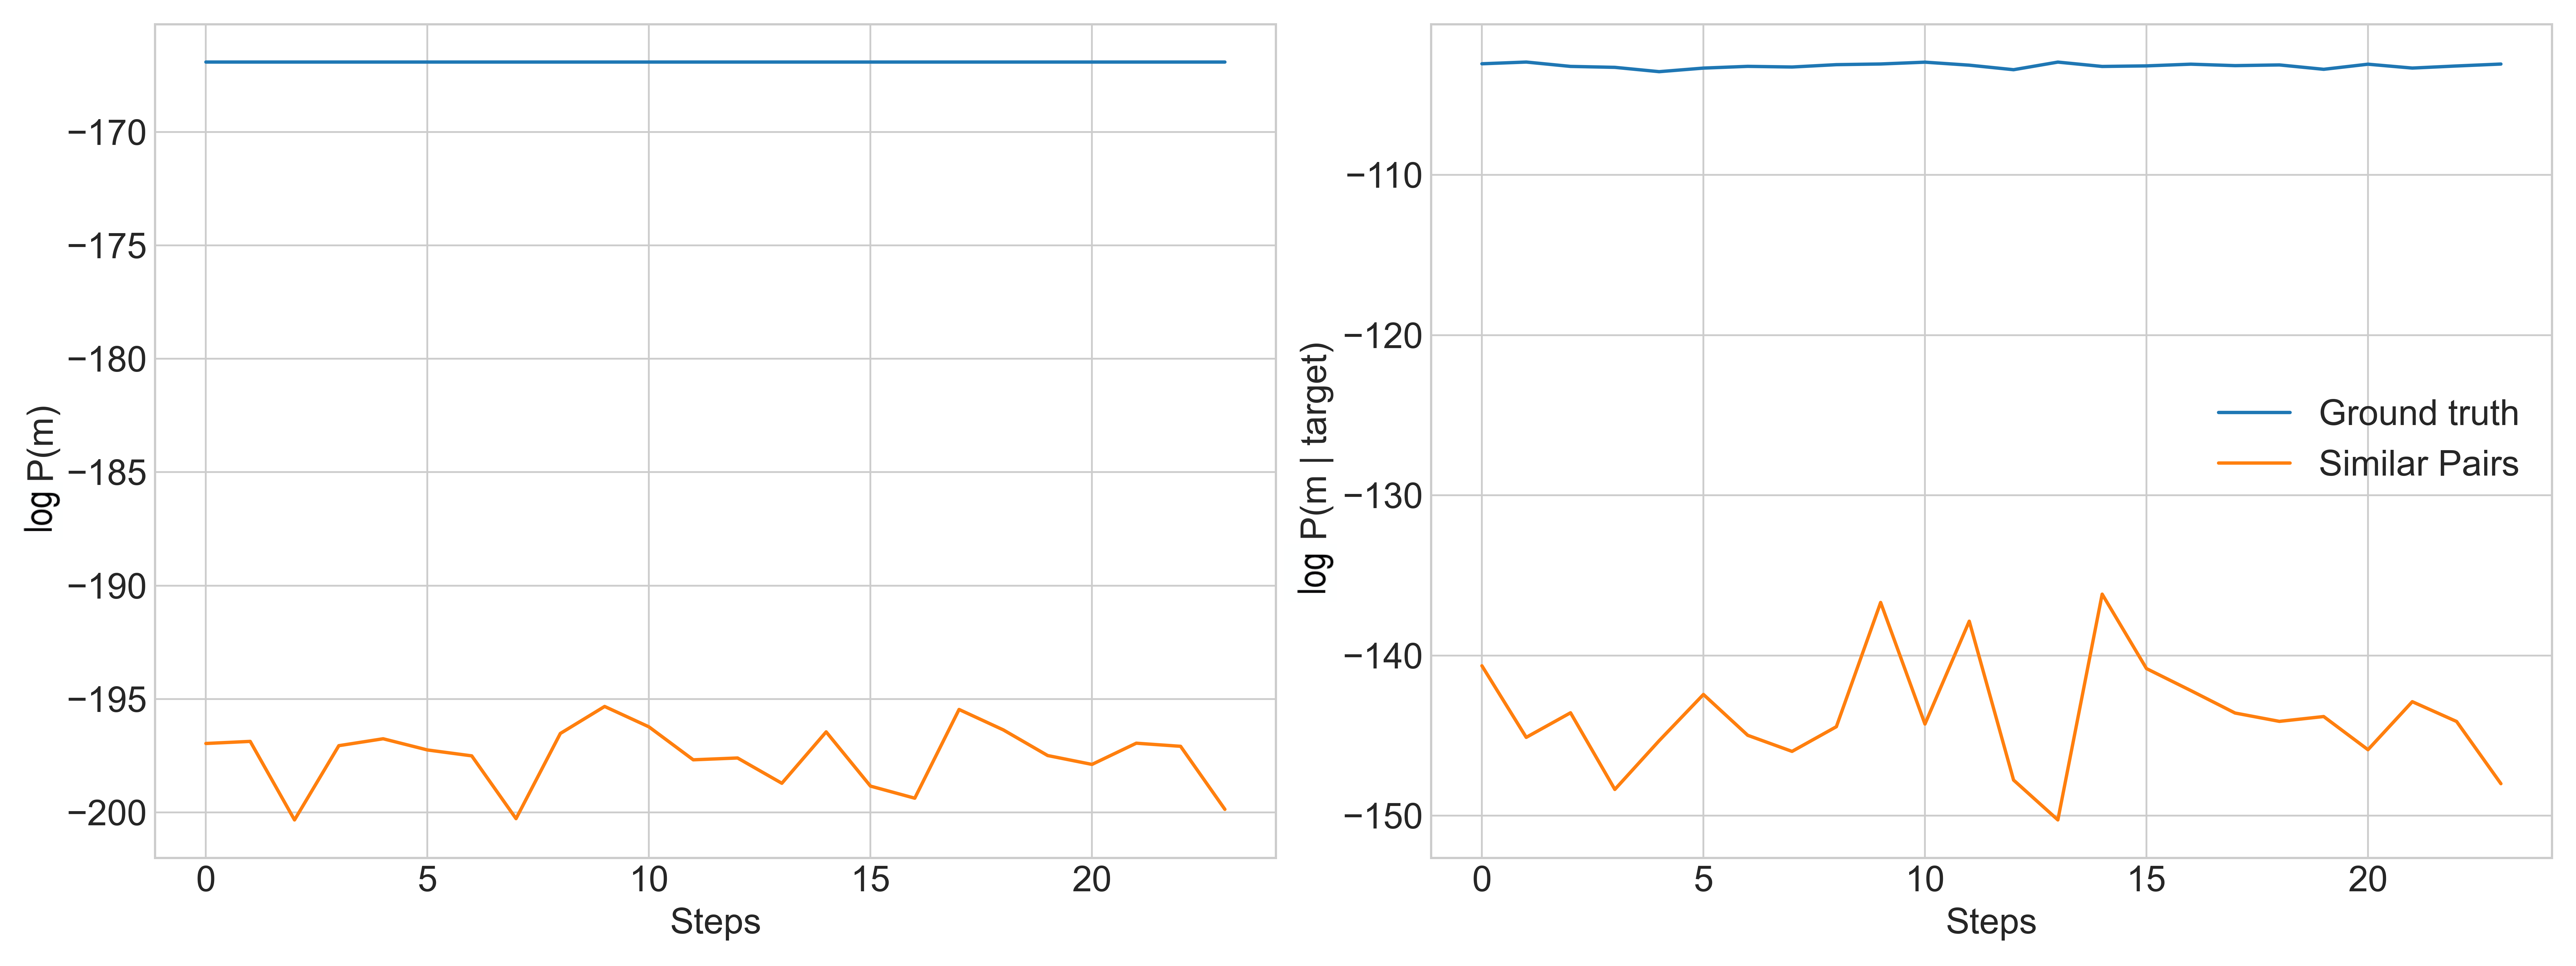
\includegraphics[width=\linewidth]{images/3dshapes_structural_semantic_drift_fixedListener_similarFixed_075.png}
	\caption{Drift dynamics computed during training of the 3Dshapes experiment on similar image pairs with fixed matching features with a fixed listener (pure decoding, exhaustive captions, $L_s = 0.75$). Left: Structural drift of ground truth and predicted captions under the pretrained LM. Right: Semantic drift of ground truth and predicted captions under the pretrained speaker model.}
	\label{fig:3dshapes_similarFixed_fixedListener_075_tr_sem_drift}
\end{figure}

To sum up, \textbf{H6} is also supported by the results of the 3Dshapes experiment with random image  pairs. Similarly to MS COCO, one can infer that reference game performance was at least partly carried by speaker-listener co-adaptation with the joint listener, and that the training signal available from the pretrained listener might both have structural effects in this smaller action space and mitigate semantic drift. 
Additionally, it was shown that training with a fixed listener on more complex visual input like similar image pairs did not provide conclusive support for \textbf{H6}, but instead revealed difficulties in grounding the joint listener in such complex input. Taken together, a complex interaction between the agents' co-adaptation, their task success capacity and the complexity of their input became apparent in these experiments.

\subsection{3DShapes: Short Captions Experiments}
\label{expt:3dshapes_short}

\begin{table}[] 
	\begin{tabularx}{\textwidth}{|X|l|l|X|X|X|X|}
		\hline
		\textbf{Model name}                                    & \textbf{log $P(m)$} & \textbf{log $P(m \mid i)$} & \textbf{Overlap (d)} & \textbf{Overlap (c)} & \textbf{Acc. (random)} & \textbf{Acc. (similar)} \\ \hline
		Ground truth mixed       &     -139.026            &    -80.323             &       7.401        &        0.028        &                 &                \\ \hline
		Pretrained 3D mixed speaker    &      -192.903           &         -59.623               &        2.309              &      -0.001                & 0.944 (baseline listeners)                 &                 \\ \hline
		%3D Baseline, random  &       -195.495        &           -147.313           &          5.247            &         0.001             & 0.979                                    &                        0.959                   \\ \hline
		%3D Baseline, similar all, $\lambda_s = 0.75$ &      -198.189             &       -140.786                 &           5.578           &        0.001              & 0.878                      &            0.906                        \\ \hline
		%3D Baseline, similar fixed, random test &       -193.709            &    -141.010                  &        3.280            &      -0.003         &            0.688       &                           \\ \hline
		%3D Baseline, similar fixed, same test &      -199.014        &        -146.280           &        2.875       &      0.029   &              &          0.691                   \\ \hline
		%3D Baseline, similar fixed, diff. test &     -194.510     &    -146.557          &   2.071      & 0.020    &                &              0.570          \\ \hline
		3D Short, random&      -189.285             &      -58.278                  &             2.316        &         0.000             &                   0.957                       &                                           \\ \hline
		3D Short, similar all, $\lambda_s = 0.75$&     -194.183        &   -59.371           &    1.032       &   0.000        &                   &         0.791       \\ \hline
		3D Short, similar fixed, random test&      -188.249           &     -121.830                  &             1.839         &         -0.001             &                   0.726                       &                                        \\ \hline
		3D Short, similar fixed, same test&      -192.130      &     -58.753      &   0.837      & 0.003      &                       &               0.723                           \\ \hline
		3D Short, similar fixed, diff. test &  -187.713       & -57.257     & 1.915        &  0.002         &      &     0.564       \\ \hline
	\end{tabularx}
	\caption{\label{tab:3dshapes_drift_metrics_basic_short} Language drift metrics and listener test accuracies (``Acc.'') of experiments on the 3Dshapes dataset including short annotations. 
		``Baseline'' refers to the setup wherein the listener is trained jointly with the speaker, using pure decoding, using exhaustive captions only. ``Random'' refers to speakers trained on random target-distractor pairs; ``similar'' refers to speakers trained on similar target-distractor pairs. $\lambda_s = 0.75$ is used in all experiments. ``Mixed'' and ``short'' refers to experiments and tests with annotation of varying lengths.}
\end{table}

The goal of these experiments was to address \textbf{H10} by conducting experiments wherein the speaker produced captions of varying granularity.
To this end, the second speaker pretrained on mixed-length captions (i.e., both exhaustive and short captions) was used (see Section \ref{speaker_pretraining}). During reference game training, the structural loss was also computed against ground truth captions of varying lengths. That is, the targets that the speaker had to refer to during training were associated with either exhaustive or short ground truth captions. Otherwise, the training followed the general procedure.

These experiments addressed several aspects. First, they addressed the question whether the presence of exhaustive captions (as was the case in the baseline experiment) was necessary for successful task completion. Second, they addressed whether absence of exhaustivity might be the reason for language drift because the speaker might have to resort to drift strategies in order to complete the functional task due to a lack of linguistic task-appropriate resources. 
Third, speaker flexibility to generate messages of variable length in absence of explicit message length regularization was investigated. 

\begin{figure}[h]
	\centering
	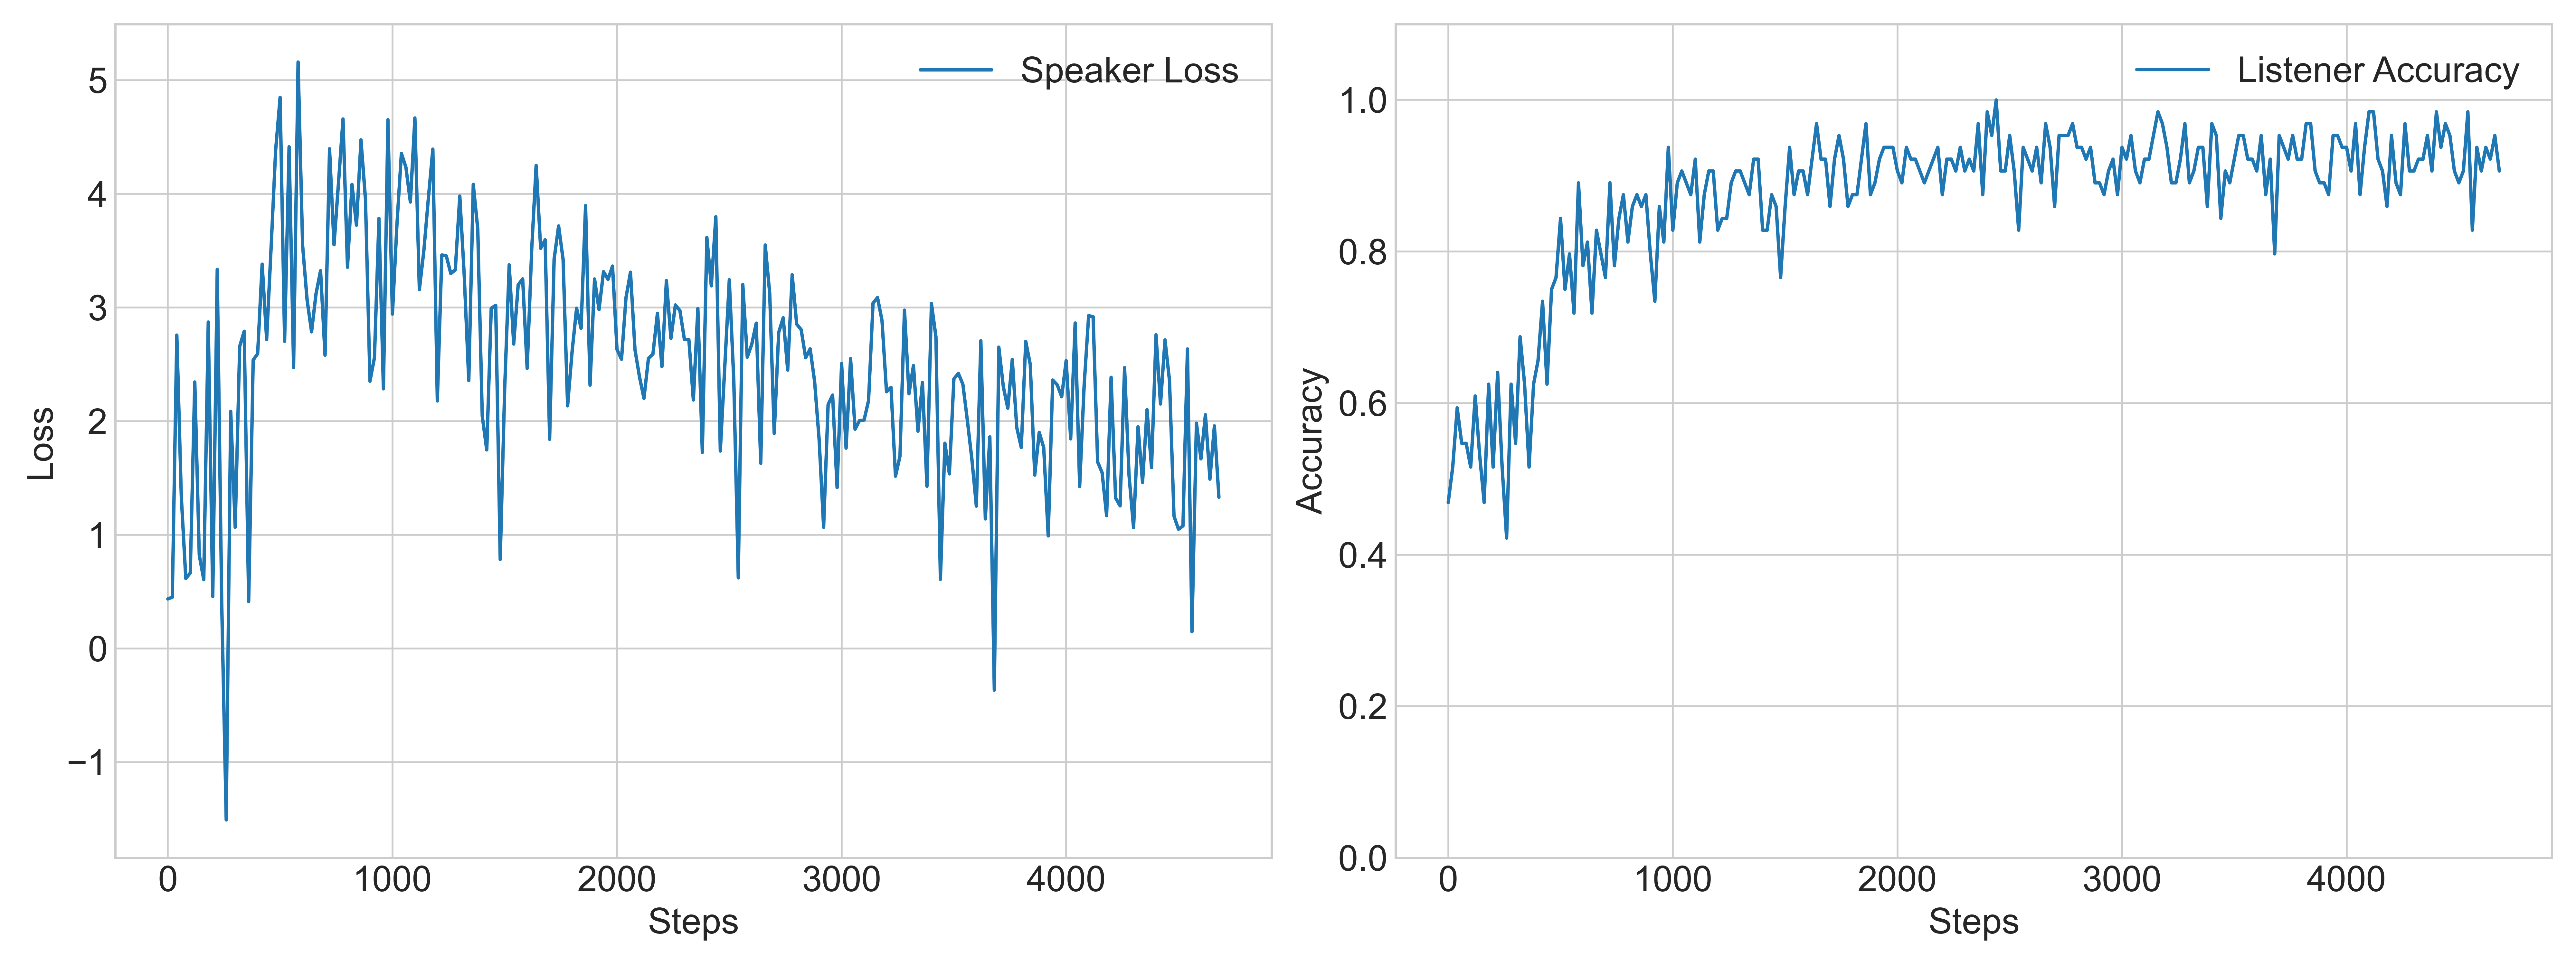
\includegraphics[width=\linewidth]{images/3dshapes_wShort_baseline_random_075_losses.png}
	\caption{Training results of the baseline reference game on both short and exhaustive captions of 3Dshapes (pure decoding, $\lambda_s=0.75$). Left: Total speaker training loss. Right: Listener training accuracy.}
	\label{fig:3dshapes_wShort_075_speaker_losses_listener_acc}
\end{figure}

First, the baseline experiment with pure decoding and $\lambda_s = 0.75$ was conducted with the mixed captions. Similar to the testing procedure in previous experiments, the model was evaluated in terms of listener accuracy and language drift on the same 1000 held out images. For the test set, it was now also chosen at random whether a target image was associated with three short or exhaustive ground truth captions out of five, in order to compute drift metrics of the ground truth captions. Therefore, the drift measures of the ground truth differ from the exhaustive ground truth captions.
The training results can be seen in Figure~\ref{fig:3dshapes_wShort_075_speaker_losses_listener_acc}. Based on visual comparison to the exhaustive captions baseline experiment (Fig.~\ref{fig:3dshapes_baseline_075_speaker_loss_listener_acc}), no qualitative differences in either speaker convergence or listener training performance could be observed. Nonetheless, listener test accuracy decreased by 0.022 compared to exhaustive baseline (Tab.~\ref{tab:3dshapes_drift_metrics_basic_short}).
This rather small difference could be because in this experiment the target and distractor images were paired at random and were, therefore, likely quite dissimilar, intuitively rendering the presence of exhaustive messages not necessary for successful reference.

Turning towards language drift, one can observe that both structural and semantic drift during training were lower for this experiment compared to the exhaustive experiment (Fig.~\ref{fig:3dshapes_wShort_075_str_sem_drift} vs. Fig.~\ref{fig:3dshapes_baseline_075_str_drift}), showing the opposite to the hypothesized effect. The lower structural drift could be attributed to generally higher naturalness of the short captions compared to the exhaustive ones, thus, rendering them more likely under a pretrained LM. The lower semantic drift which additionally was lower for the generated captions than for the ground truth ones might indicate that the speaker was further fine-tuned to produce messages that were more likely under the pretrained speaker generation strategy. This might be easier than for exhaustive captions because of the shorter effective message length which is advantageous for RNN training \parencite[cf.][]{jaeger2002tutorial}. This is further cofirmed by the test drift results. Structural drift was lower compared to both the exhaustive baseline and the pretrained speaker. However, the absolute difference to the drift value of the ground truth captions was much larger for mixed captions (50.259) compared to the exhaustive captions (30.743) (Tab.~\ref{tab:3dshapes_drift_metrics_basic_short}). This might suggest that due to the varying length of messages and the respective variation in sentence structure the speaker might struggle more to produce syntactically well-formed sentences after fine-tuning. 
Similarly, semantic drift was lower for mixed captions compared to the both exhaustive and pretrained speakers. The absolute difference in semantic drift of the fine-tuned speaker and the ground truth captions was 22.045 for mixed captions and 39.457 for the exhaustive experiment, where in the former the speaker actually improved over ground truth captions, while the latter was worse (Tab.~\ref{tab:3dshapes_drift_metrics_basic_short}). This might indicate that further supervised fine-tuning of the speaker model took place for the mixed but not the exhaustive captions. Again, this could be attributed to the effective message length difference of the ground truth captions and the respective difficulty of training.
Regarding overlap metrics, the discrete overlap decreased much more drastically compared to ground truth for the mixed captions than for exhaustive ones. This low value might be confounded with the variation of the granulaity of a sampled ground truth caption, and not be directly representative of functional performance. For instance, during evaluation, the speaker might have generated a valid discriminative short caption, but the sampled corresponding ground truth was an exhaustive caption, yielding a low overlap value. Overall, however, absence of exhaustive captions did not lead to `strategic' language drift.  

\begin{figure}[h]
	\centering
	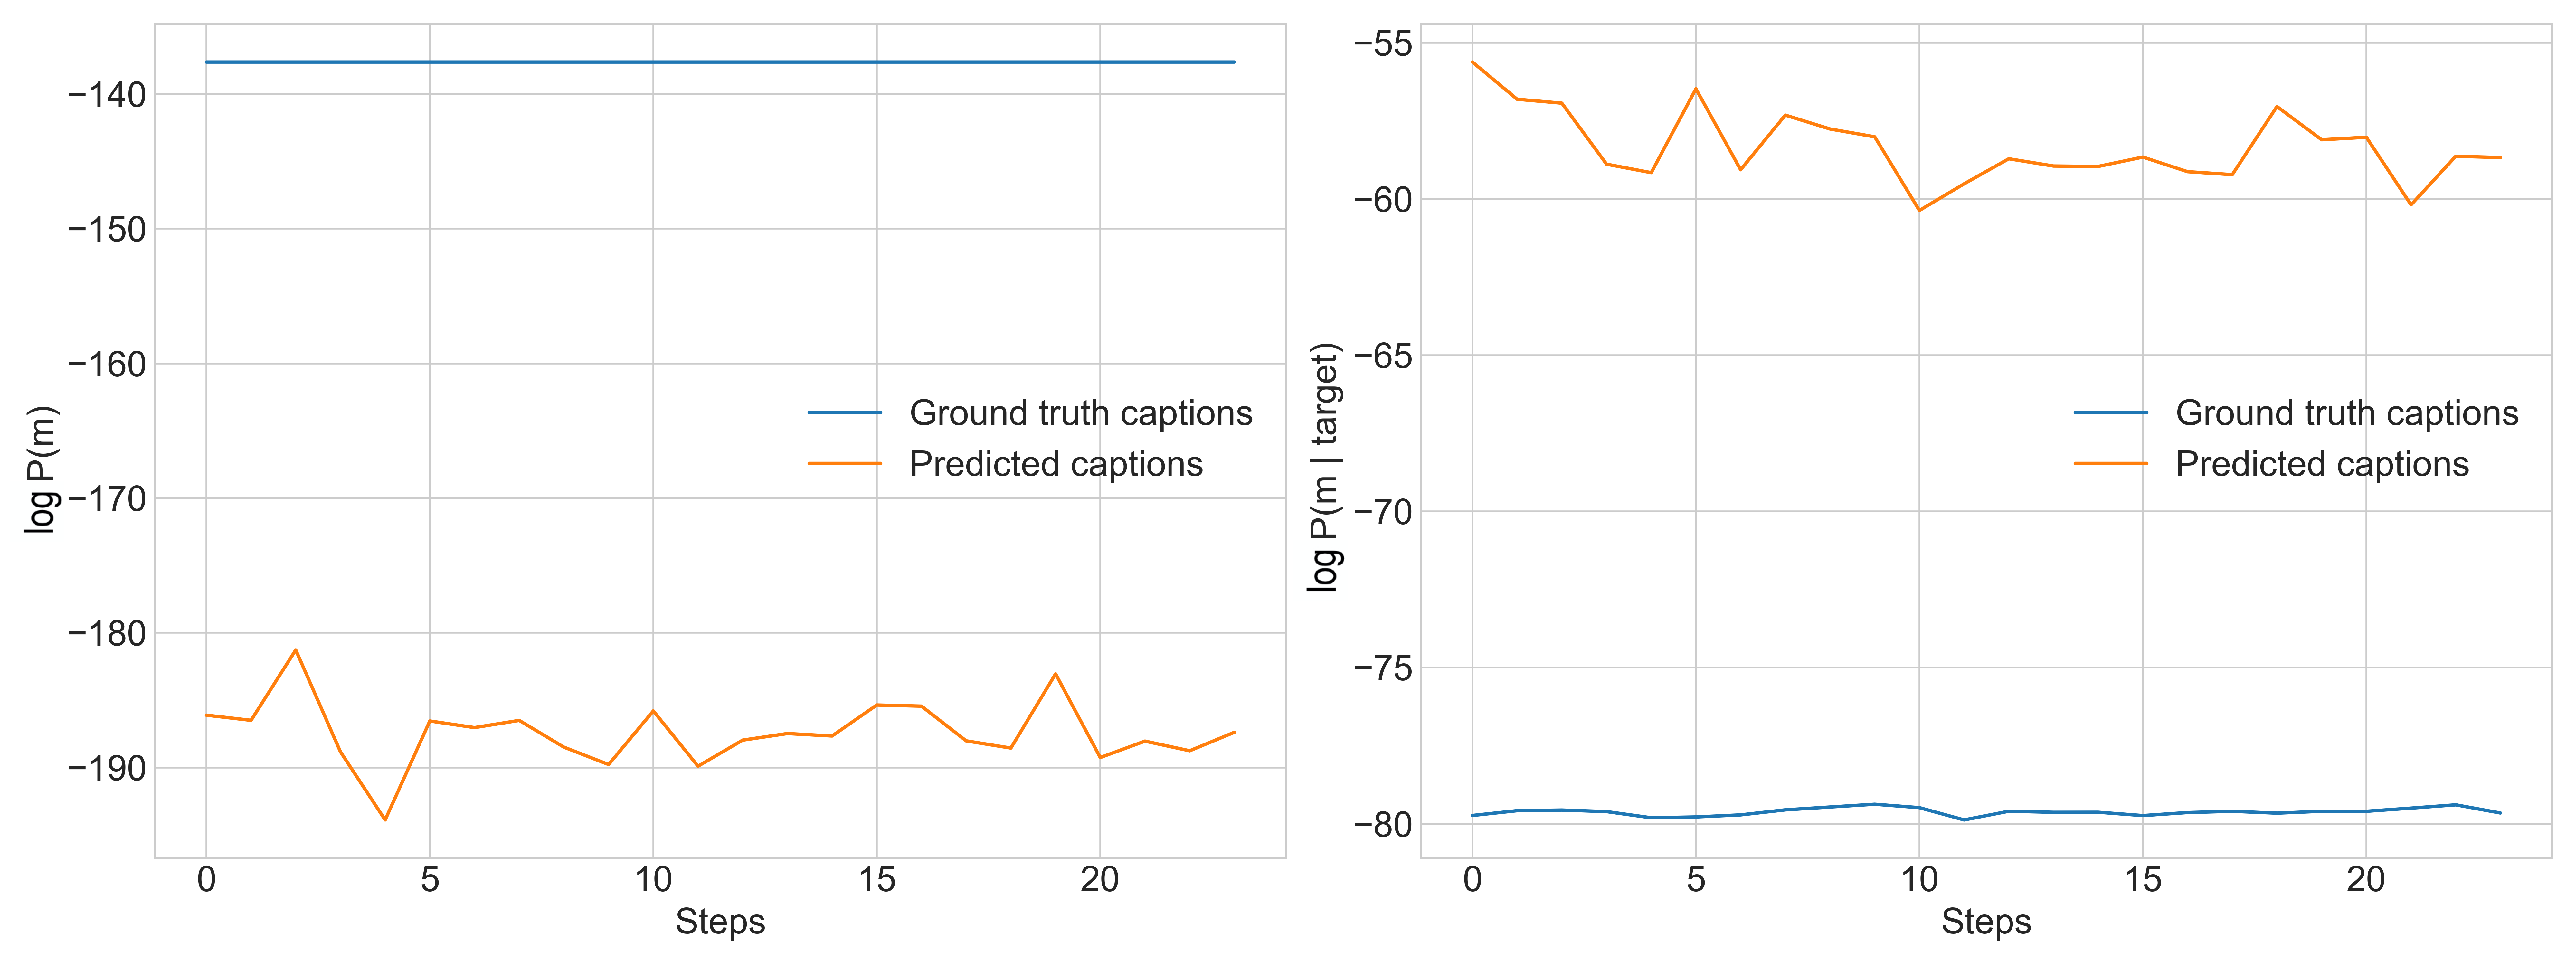
\includegraphics[width=\linewidth]{images/3dshapes_wShort_structural_semantic_drift_49_pure_075_random.png}
	\caption{Drift dynamics computed during reference game training on both short and exhaustive captions of 3Dshapes (pure decoding, $\lambda_s=0.75$). Higher values indicate less drift. Left: Structural drift of ground truth and predicted captions under the pretrained LM. Right: Semantic drift of ground truth and predicted captions under the pretrained speaker model.}
	\label{fig:3dshapes_wShort_075_str_sem_drift}
\end{figure}

In order to investigate the third aspect---speaker's generation length flexibility---lengths of the captions generated by the speaker on the validation set were computed. These were calculated by counting the number of tokens until the first occurrence of the special END token in the message (excluding it). As can be seen in Figure~\ref{fig:3dshapes_exh_short_random_lengths}, the speaker that saw short captions during pretraining and in the reference game has learned to produce captions with varying length with approximately uniform probability, except for a bias towards generating captions of maximal allowed length around one third of the time. This bias can also be observed for the exhaustive captions speaker, whose generated caption lengths matched the ones from the exhaustive training set. These results hint at the importance of the training data distribution for the speaker's potential to adjust her message length, possibly responding to different granularity needs (see Section \ref{expt:3d_similar} for details). 

\begin{figure}[h]
	\centering
	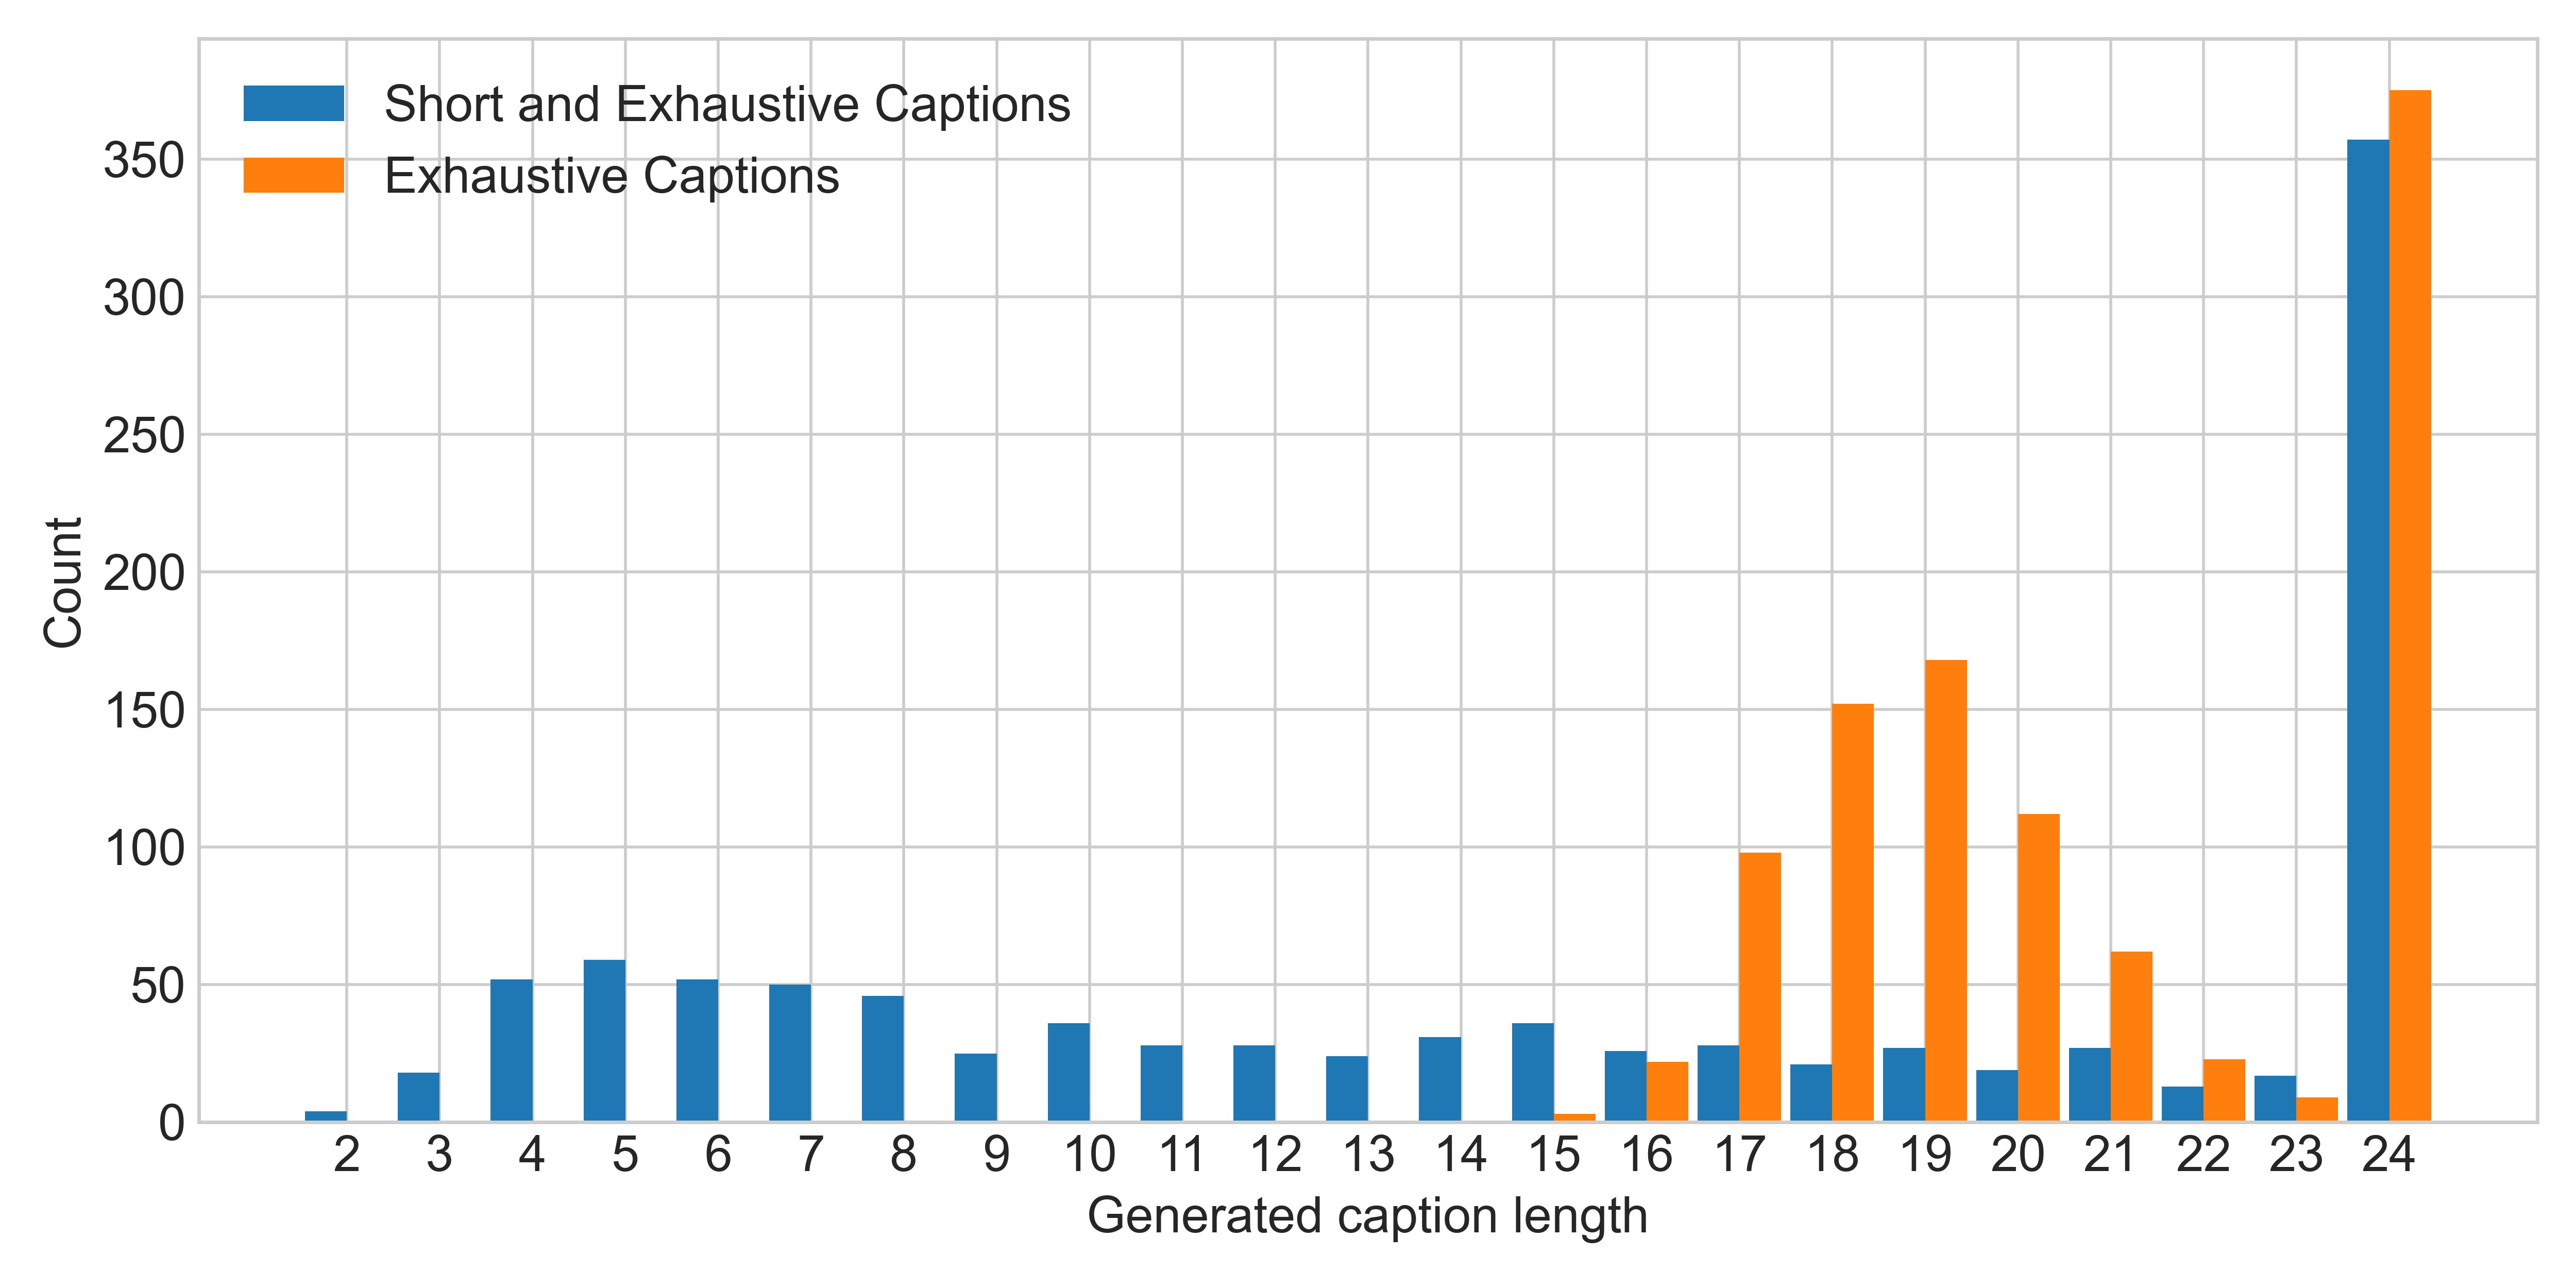
\includegraphics[width=0.7\linewidth]{images/3dshapes_exh_short_random_length_counts.png}
	\caption{Counts of effective sentence lengths generated on the validation dataset by the speakers from the exhaustive and the mixed-length experiments.}
	\label{fig:3dshapes_exh_short_random_lengths}
\end{figure}

In sum, \textbf{H10} was not supported by experimental results on random target-distractor pairs. In fact, language drift was even smaller compared to the exhaustive captions experiment. This suggests that architectural aspects like the length of messages the speaker was trained to generate have a larger influence on message quality than guaranteed presence of fully descriptive captions in the training dataset. At the same time, these results showed that the speaker was capable of flexibly varying her message length, if the respective inductive bias was provided during training. 

\subsubsection{Similar Pairs Experiment}
\label{expt:3d_similar}

In order to increase the pressure towards the necessity of exhaustive descriptions, an experiment including short captions was conducted on \emph{similar} target-distractor image pairs. Again, the similar pairs were constructed such that the target and the distractor matched with respect to object shape, object color and background color. Since this set up allows for more detailed analyses, the set up akin to the first experiment in Section \ref{expt:3dsapes_similar} (where all features were used for matching the pairs) is omitted for the mixed captions. The results of the comparable similar pairs experiment with exhaustive captions are discussed in Section \ref{expt:3dsapes_similar}. The effect of adding short captions during training compared to using exhaustive captions only can be seen in Figure~\ref{fig:3dshapes_wShort_similarFixed_075_speaker_losses_listener_acc} which shows that training the speaker on mixed length captions did not visibly influence the training dynamics compared to exhaustive captions only. However, similarly to exhasutive captions results, the listener's test performance on held out image pairs, both matching along the same and along different features, was much worse than training accuracy (0.723 and 0.564, respectively, see Tab.~\ref{tab:3dshapes_drift_metrics_basic_short}). This discrepancy was comparable to the exhaustive experiments, indicating that potential overfitting cannot be attributed to the difficulty of learning longer messages. Language drift results in Table \ref{tab:3dshapes_drift_metrics_basic_short} indicated a lower structural drift than for the exhaustive speaker compared to the respective pretrained speaker, suggesting that this drift is driven by message length as in the random pairs experiments, and is not as much influenced by perceptual context. Just as in the case of the exhaustive speaker in the similar pairs experiment, semantic drift also did not increase compared to the pretrained speaker, so no speaker-listener co-adaptation was observed. However, similarly to the random pairs experiment including mixed length captions, the semantic drift of the generated captions was tangibly lower than the drift of the ground truth captions (Tab.~\ref{tab:3dshapes_drift_metrics_basic_short}), which already became apparent during training (Fig.~\ref{fig:3dshapes_wShort_similarFixed_075_str_sem_drift}, right, red line being above the yellow line). Following the random pairs experiment, this could be attributed to easier training of the speaker on shorter messages and resulting further fine-tuning of the speaker during the reference game, even on complex visual input. 

In this experiment, a larger discrete overlap can be observed for the different features test set than for the same features test set, and no increase in continuous overlap compared to baseline can be seen. This might suggest that the speaker can more easily fall back to the messages applicable to different features which were learned during pretraining when the messages are shorter. On the other hand, this might indicate that the speaker was more successful in learning to refer to novel features not present in the ground truth captions with shorter messages, compared to the random pairs experiment with short captions. So the first two aspects of the short captions experiments were not influenced much by the similar pairs input, compared to the random pairs results.
\pt{Image caption evaluations tbd}
\begin{figure}[h]
	\centering
	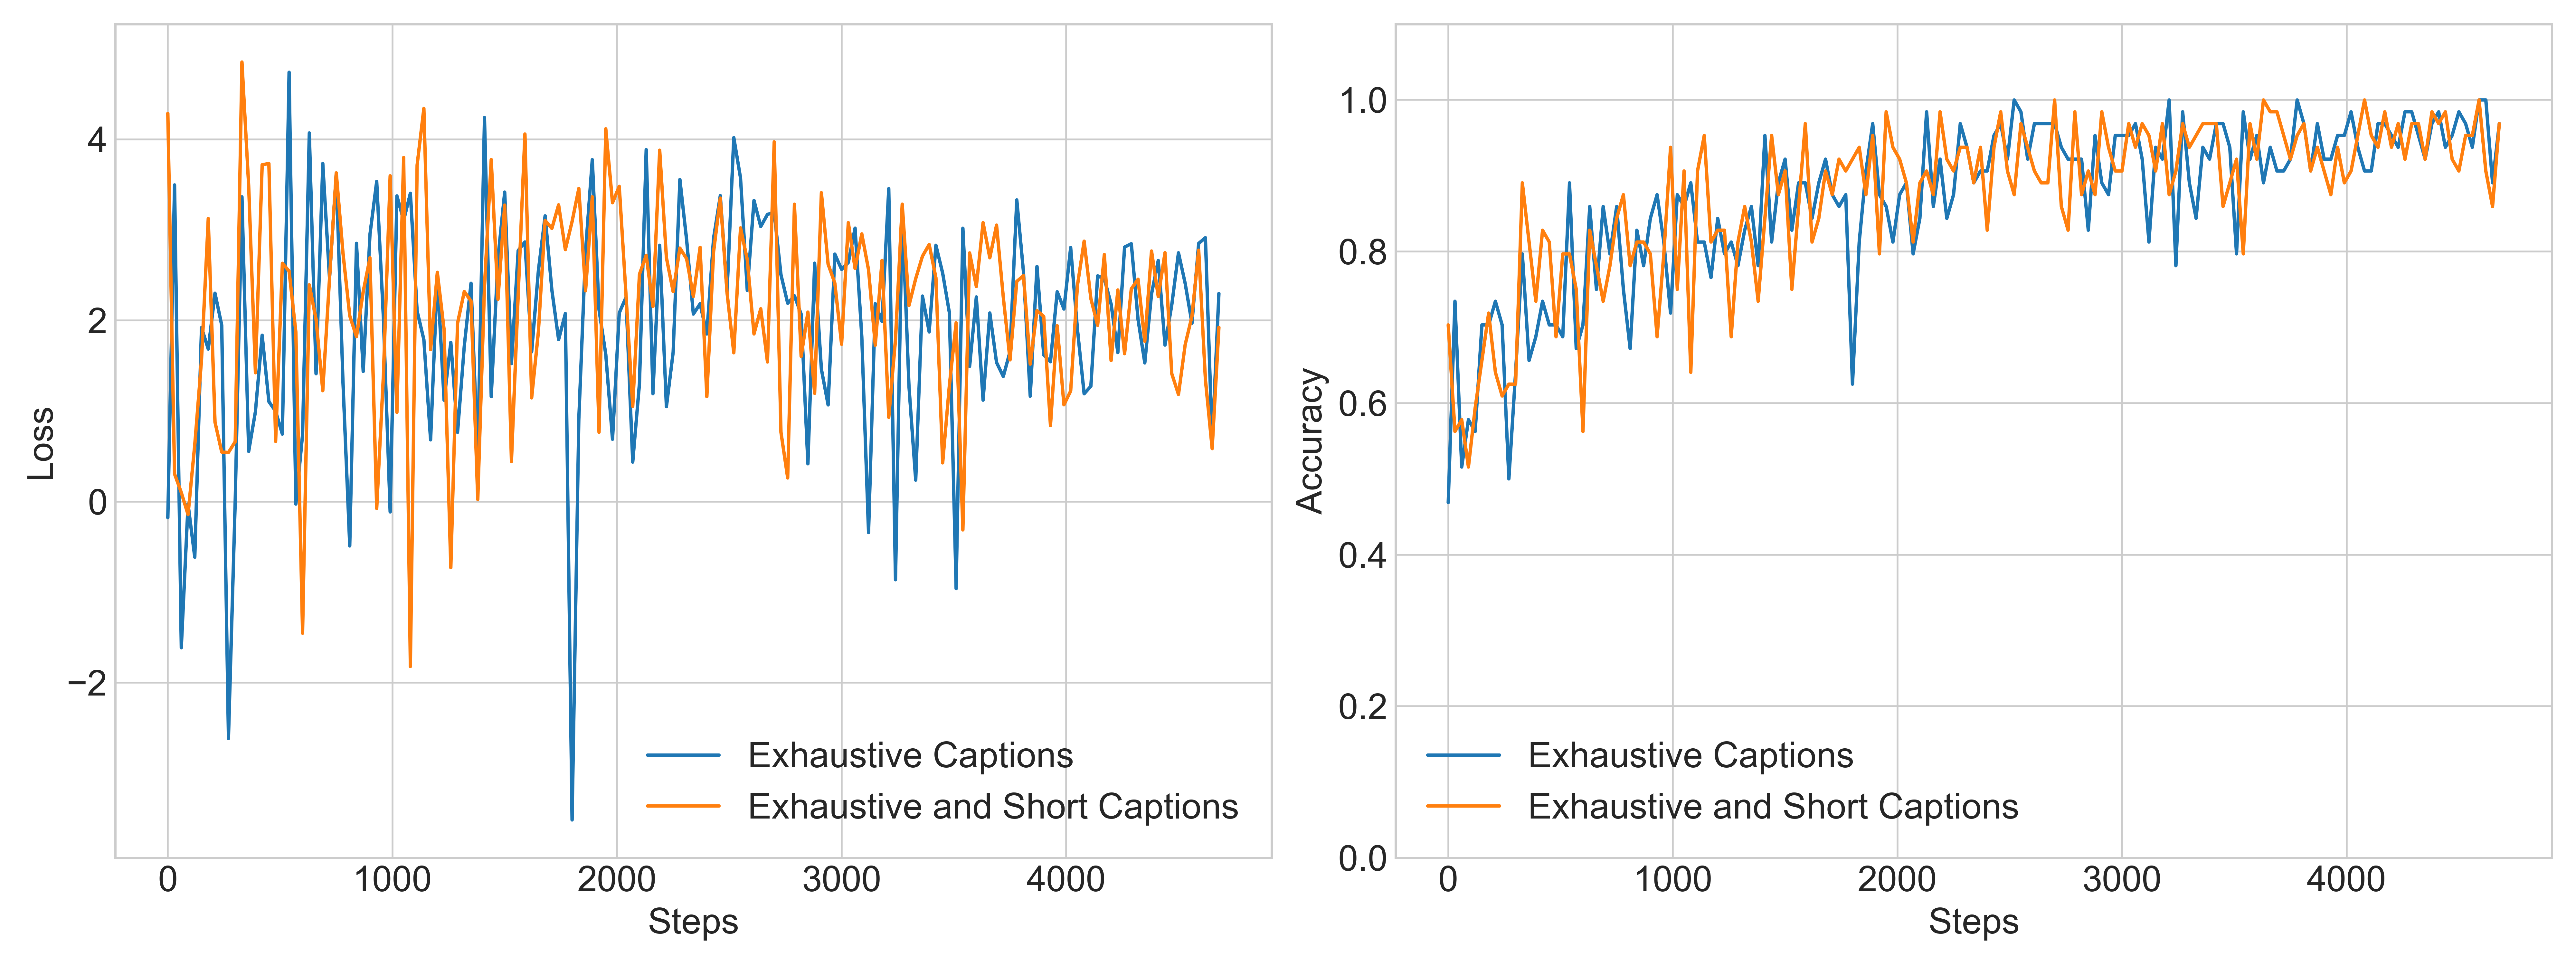
\includegraphics[width=\linewidth]{images/3dshapes_similarFixed_short_vs_exh_075_losses.png}
	\caption{Training results of the baseline reference game on both short and exhaustive captions of 3Dshapes on similar image pairs. Similar features were fixed (pure decoding, $\lambda_s=0.75$). Left: Total speaker training loss. Right: Listener training accuracy.}
	\label{fig:3dshapes_wShort_similarFixed_075_speaker_losses_listener_acc}
\end{figure}

\begin{figure}[h]
	\centering
	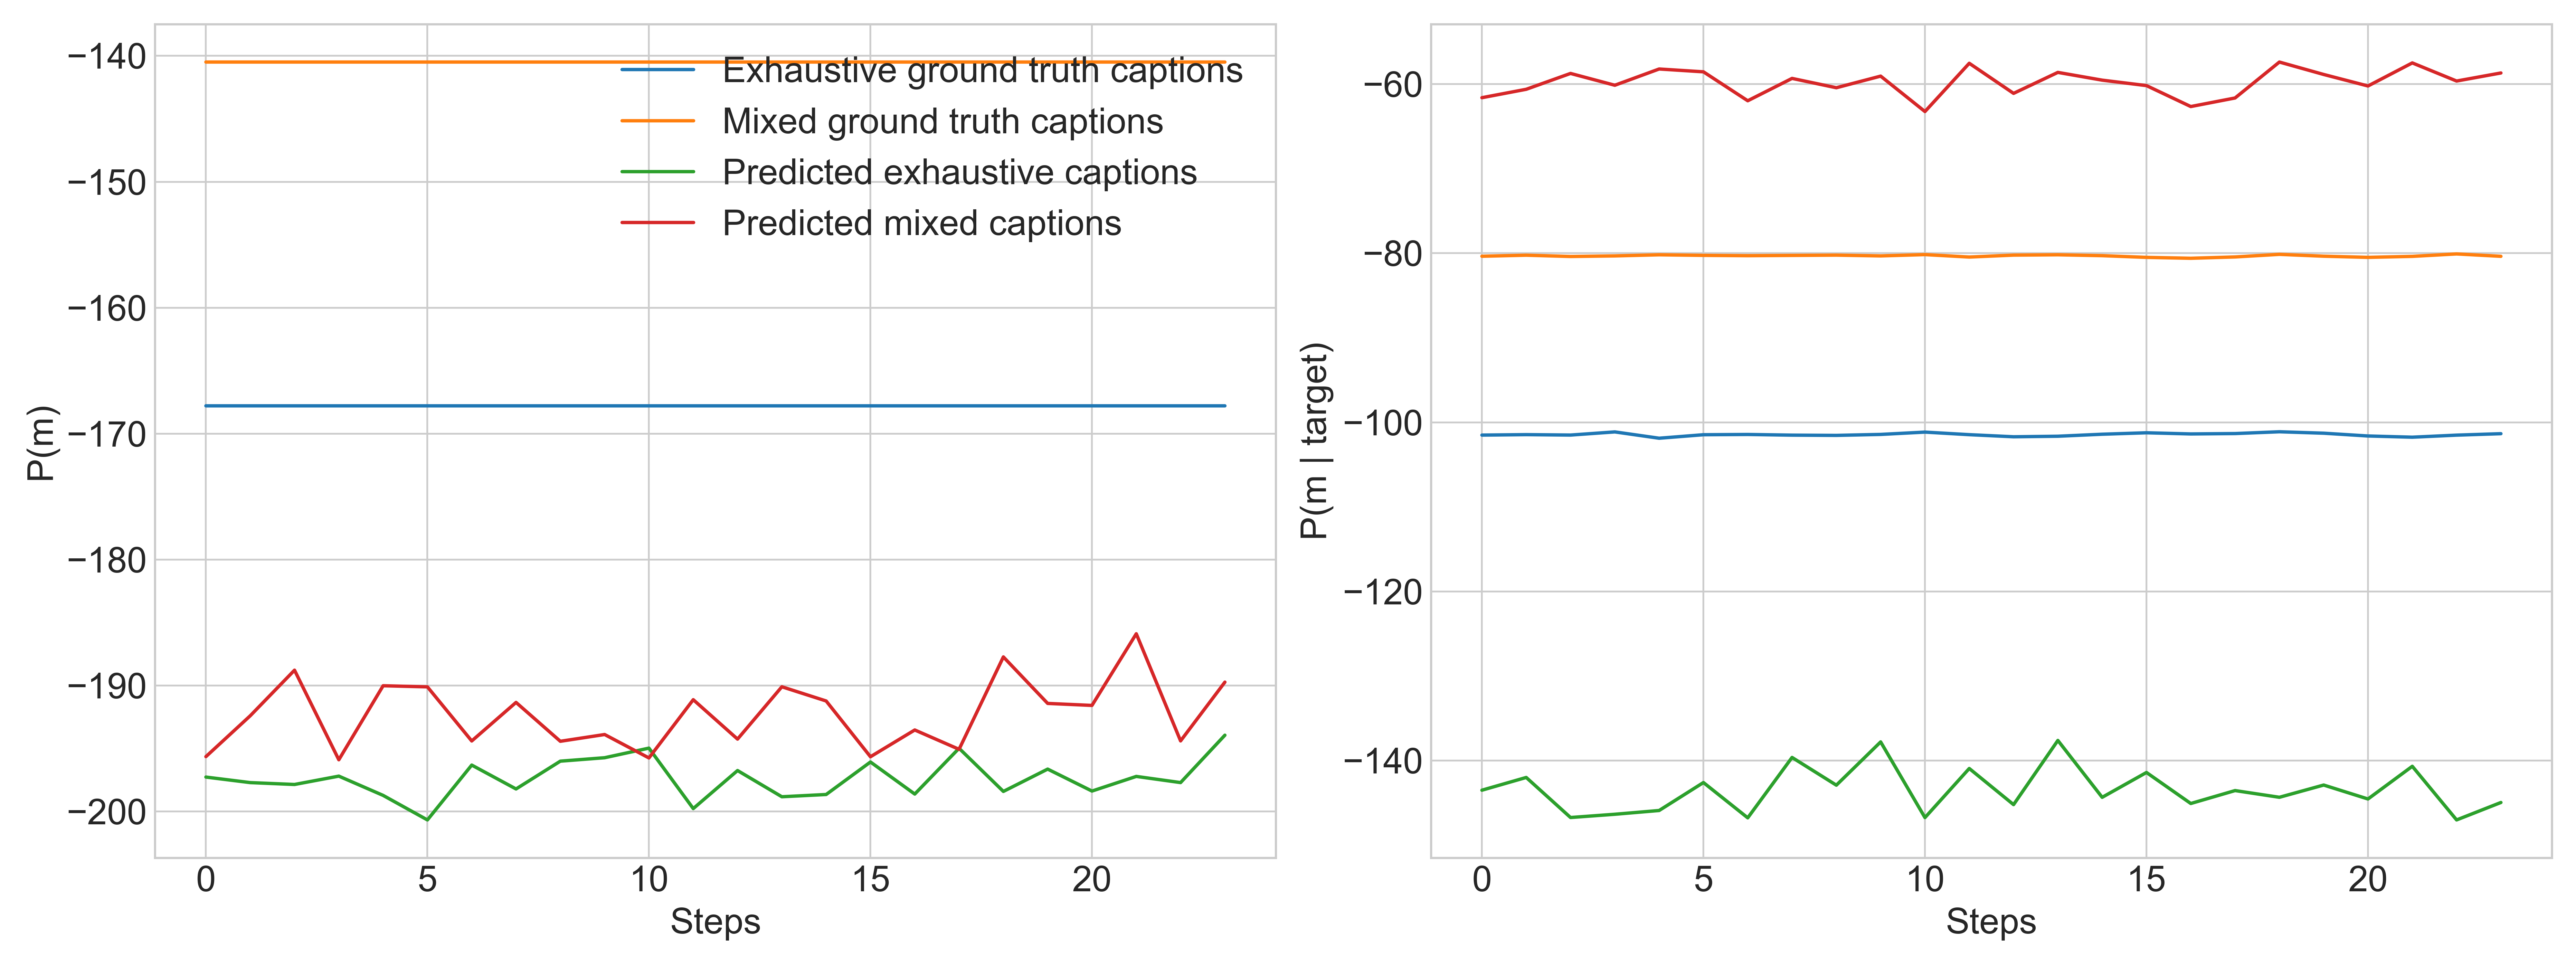
\includegraphics[width=\linewidth]{images/3dshapes_exh_short_structural_semantic_drift_49_pure_075_similarFixed.png}
	\caption{Drift dynamics computed during reference game training on both short and exhaustive captions of 3Dshapes (pure decoding, $\lambda_s=0.75$). Higher values indicate less drift. Left: Structural drift of ground truth and predicted captions under the pretrained LM. Right: Semantic drift of ground truth and predicted captions under the pretrained speaker model.}
	\label{fig:3dshapes_wShort_similarFixed_075_str_sem_drift}
\end{figure}

\begin{figure}[h]
	\centering
	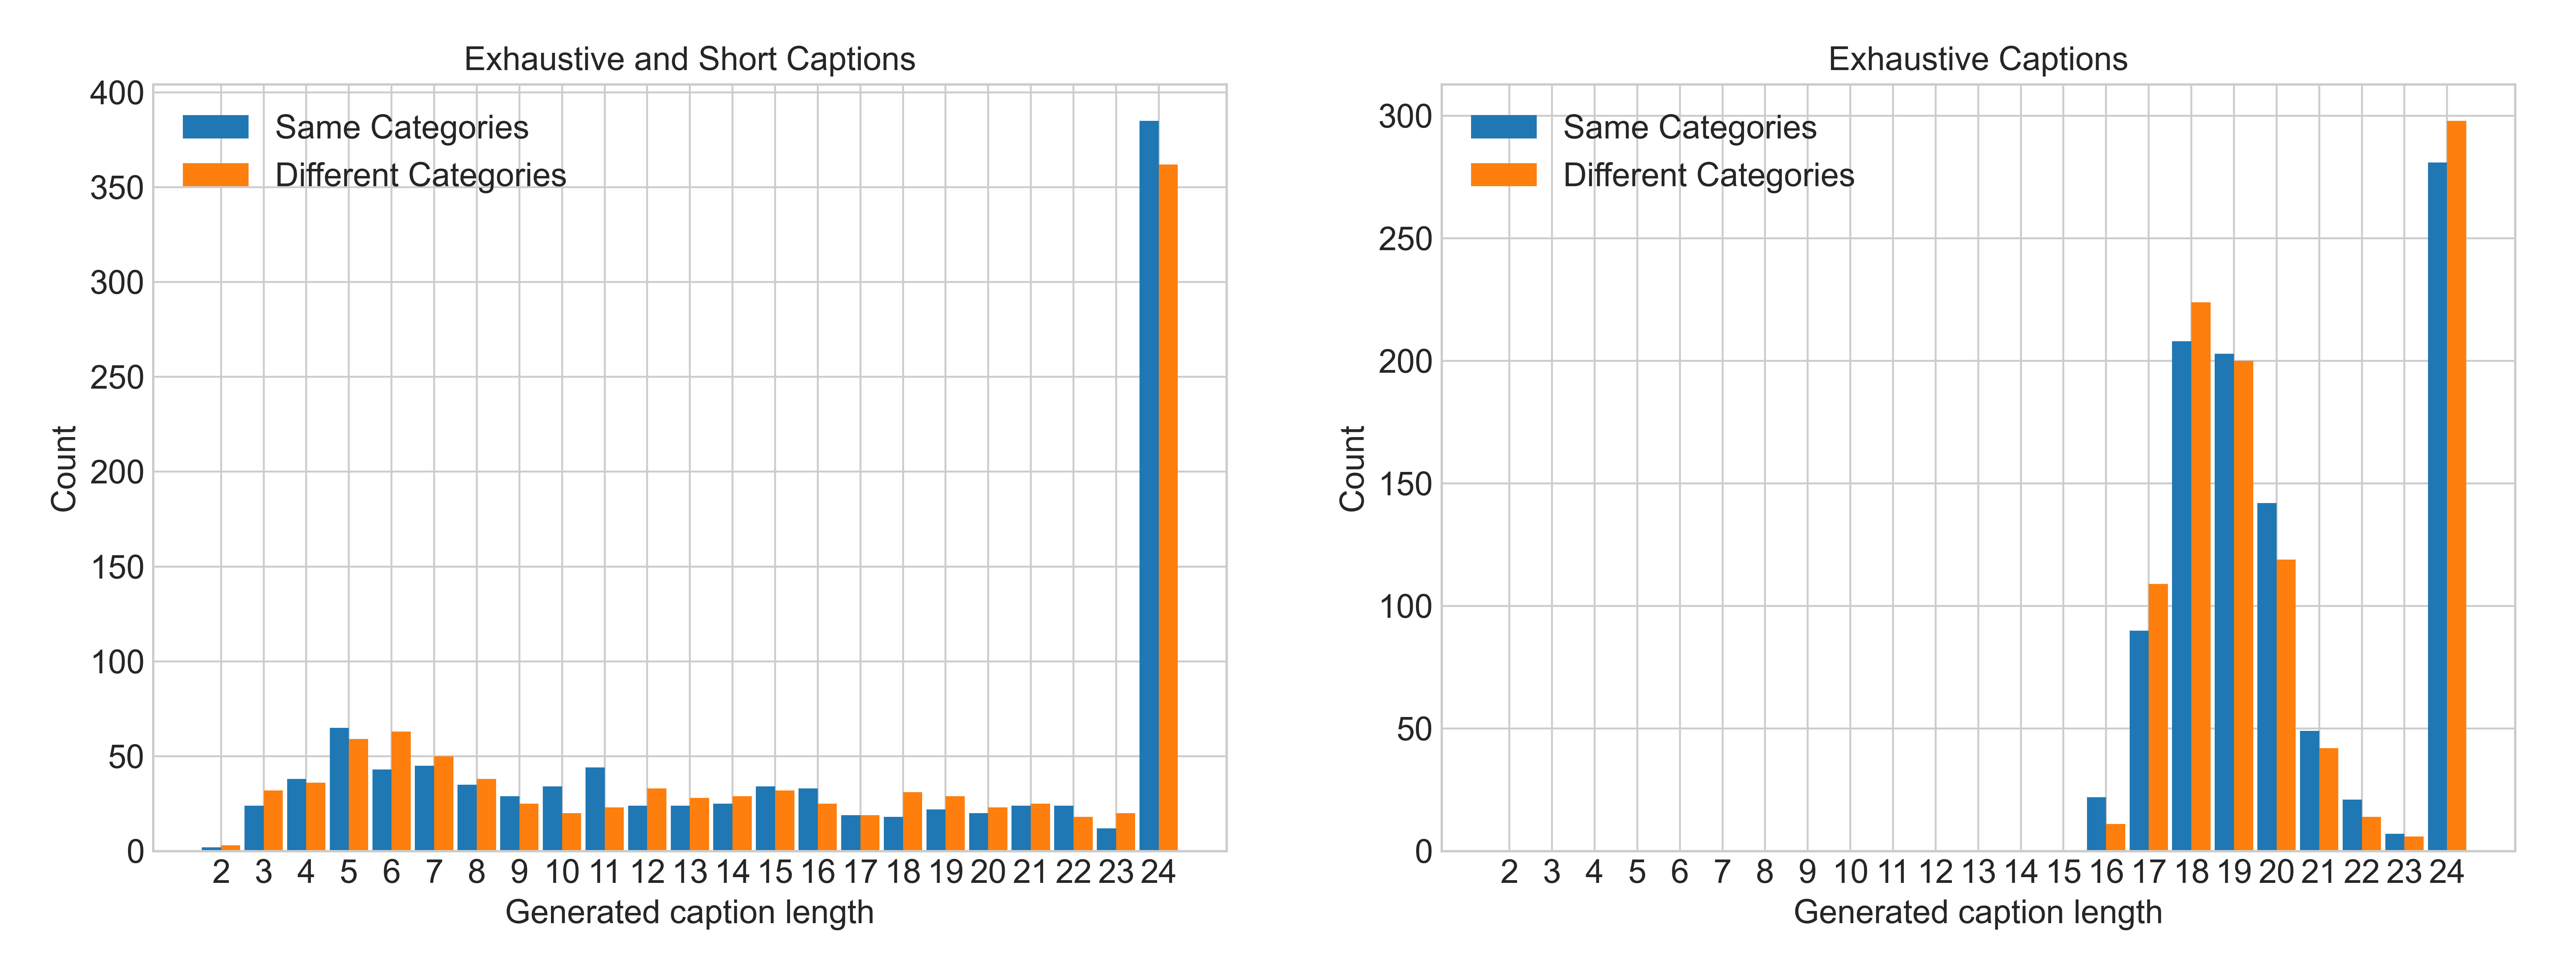
\includegraphics[width=\linewidth]{images/3dshapes_exh_short_similar_sameTest_diffTest_length_counts.png}
	\caption{Generated caption lengths for the mixed captions (left) and exhaustive (right) speakers trained in the similar pairs experiment on 3Dshapes. The test images were either similar along the same features as the training image pairs, or along the other three features.}
	\label{fig:3dshapes_exh_short_same_diff_lengths}
\end{figure}

\begin{figure}[h]
	\centering
	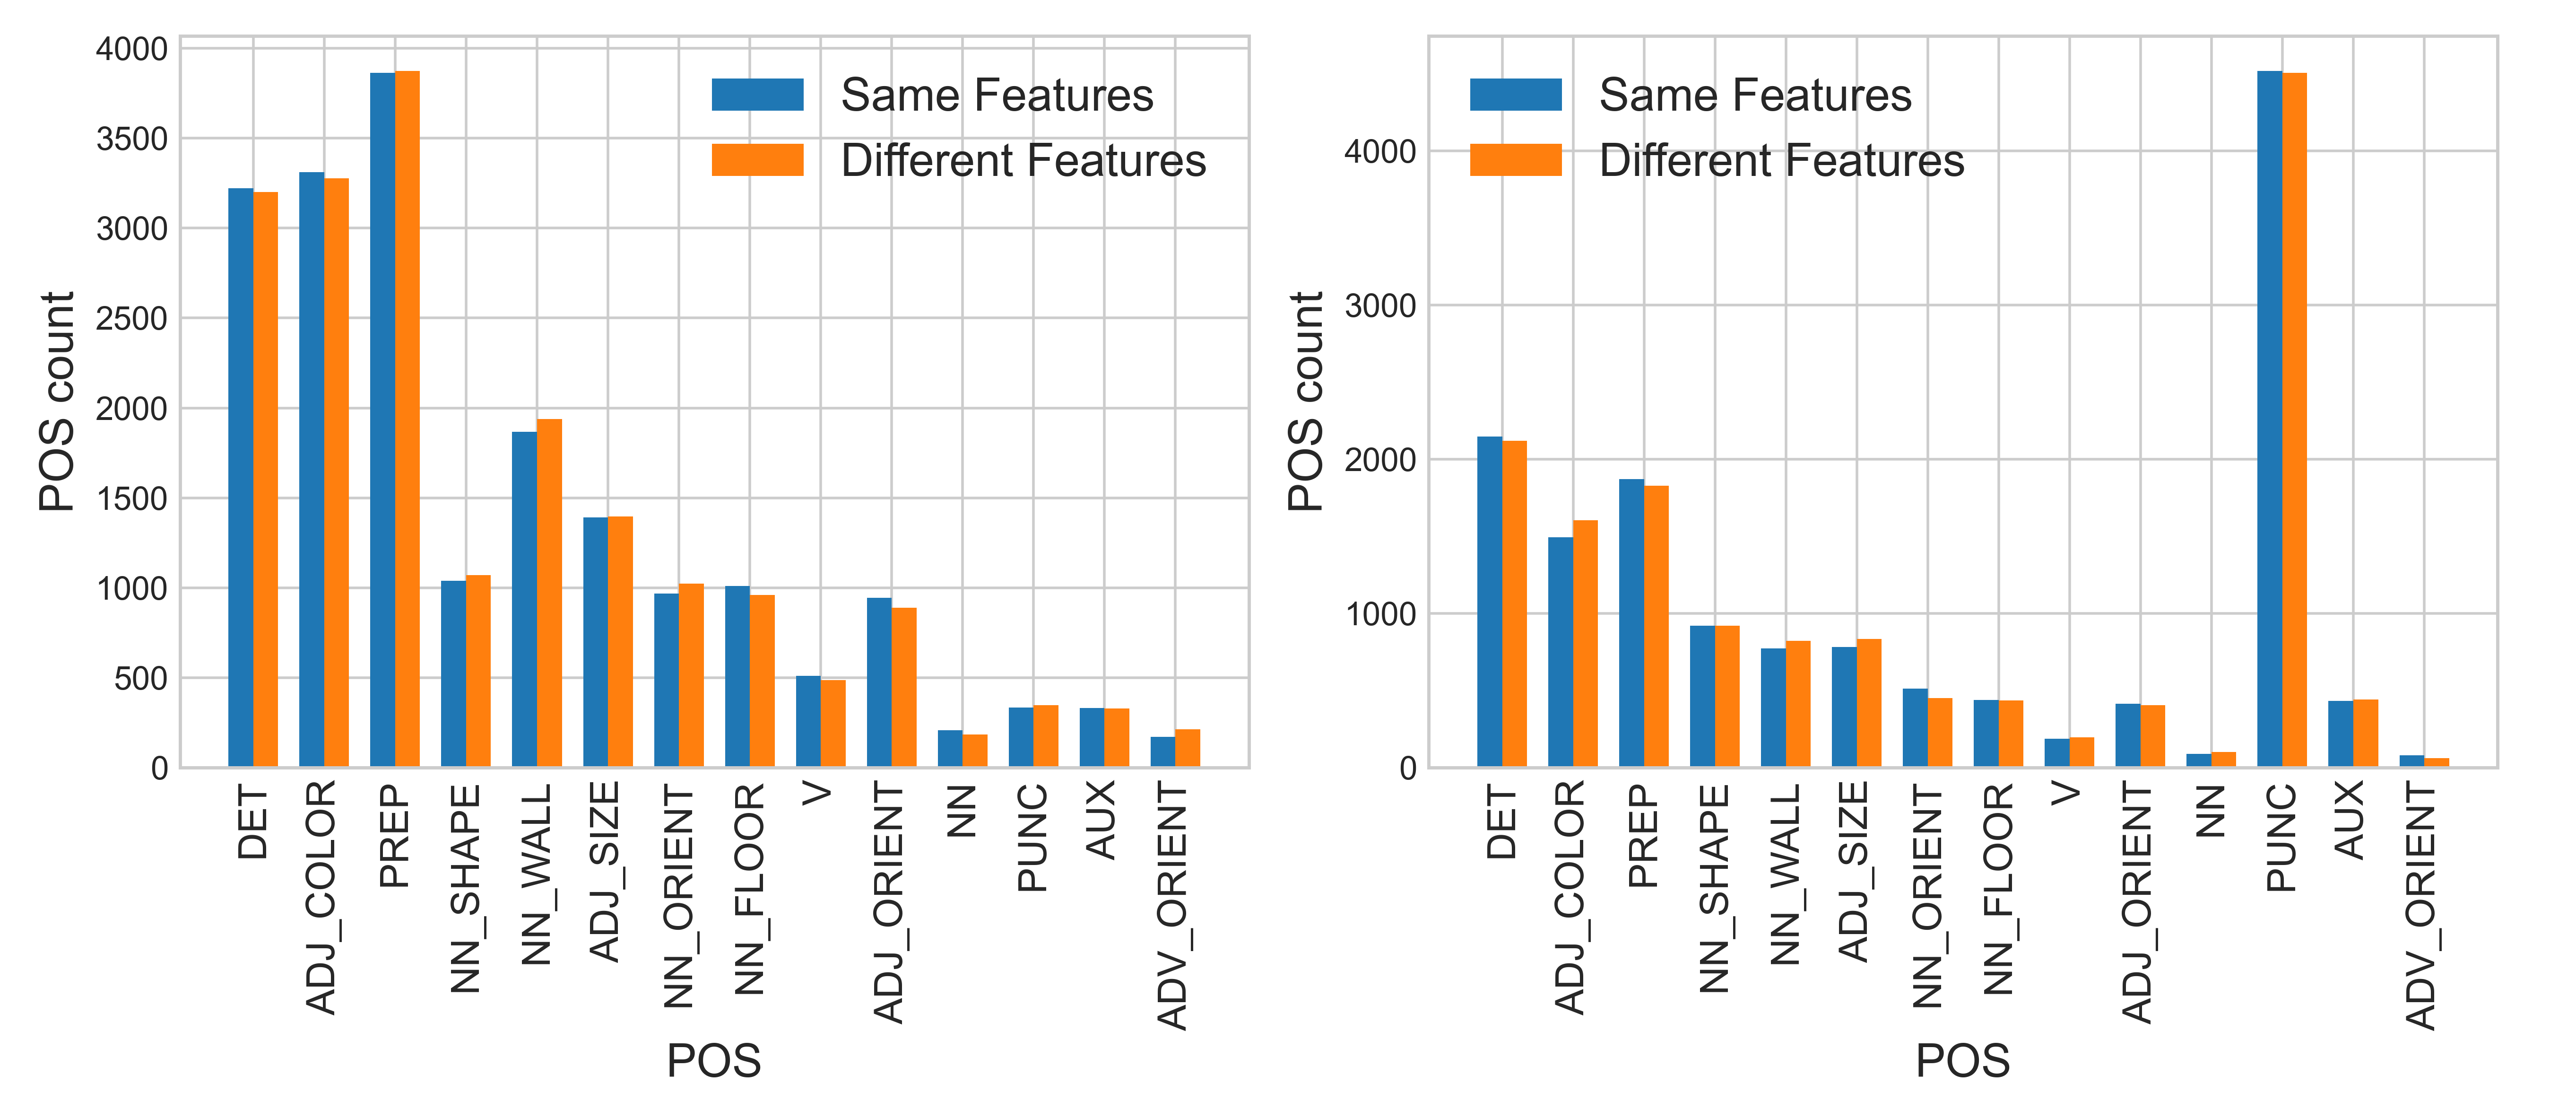
\includegraphics[width=\linewidth]{images/3dshapes_similarFixedPairs_exh_vs_short_sameTest_vs_diffTest_POS_counts.png}
	\caption{POS counts in captions produced by speakers trained on image pairs matching w. r. t. fixed features, tested on images matching on the same features (blue)~vs.~on different features (orange). Left: Speaker trained with exhaustive captions only. Right: Speaker trained with both short and exhaustive captions.}
	\label{fig:3dshapes_exh_short_same_diff_POS}
\end{figure}

Addressing the main question whether the speaker could flexibly adjust the granularity of her messages based on the difficulty of referring to discriminative features and if this required exhaustive captions, Figure \ref{fig:3dshapes_exh_short_same_diff_lengths} (left) shows a small trend towards longer messages for the different features test set compared to the same features test set. Therefore, the speaker learned to flexibly adapt her message length. However, this flexibility did not increase with the presence of both short and long annotations since the extent of the flexibility matches the exhaustive annotations experiment (Fig.~\ref{fig:3dshapes_exh_short_same_diff_lengths}, left~vs.~right). 
Investigating whether the speaker was able to refer to different discriminative aspects depending on the test set, the speaker's respective messages were POS-tagged (Fig.~\ref{fig:3dshapes_exh_short_same_diff_POS}, comparing the exhaustive speaker from Section \ref{expt:3dsapes_similar} to the current mixed lengths one). Again, the discriminative features for the same features test set were the color of the floor, the orientation and the size of the object. For the different features test set, these were the color of the background (i.e., wall), the object's color and its type. The differences in the occurrence frequencies were marginal, yet following intuition, %the exhaustive speaker referred to the floor (``NN\_FLOOR'' tag) and the orientation of the object (``ADJ\_ORIENT'', ``ADV\_ORIENT'') more frequently for the same test set than for the different test set. This was not the case for the size of the object (``ADJ\_SIZE''). 
the mixed lengths speaker referred to the orientation (``NN\_ORIENT'') of the same test targets more frequently than for different features targets. Different from the exhaustive speaker, the speaker did not prefer floor descriptions. 
For the different features test set, both speakers referred to the wall more frequently (``NN\_WALL''), but only the exhaustive speaker also had a preference for the object type (``NN\_SHAPE''). Another apparent difference between the speakers was the preference for the use of fullstop and determiners (``PUNC'', ``DET''), suggesting that the mixed speaker might have more difficulties in predicting the proper end of the sentence.
The distribution of color references would require a more detailed analysis in order to disentangle which part of the image it might apply to. Taken together, these results indicate that the mixed length speaker was also capable of identifying discriminative features of the images, but it was easier for the exhaustive speaker. Again, given that there was no difference in this capacity between the two test sets for the mixed length speaker, one could hypothesize that this flexibility was also driven by the skills from pretraining rather than reference game based adaptation. 

In sum, this is a promising result showing that it may not be necessary to have completely exhaustive, almost task-specific, annotations for the agents to learn to flexibly adjust the length of their messages---they can be trained to do so via learning from interaction in variable visual contexts. However, more exhaustive captions are more advantageous for teaching the speakers to adapt their message granularity in response to contextual needs via mentioning different attributes, and not the message length.

%\begin{figure}
%	\centering
%	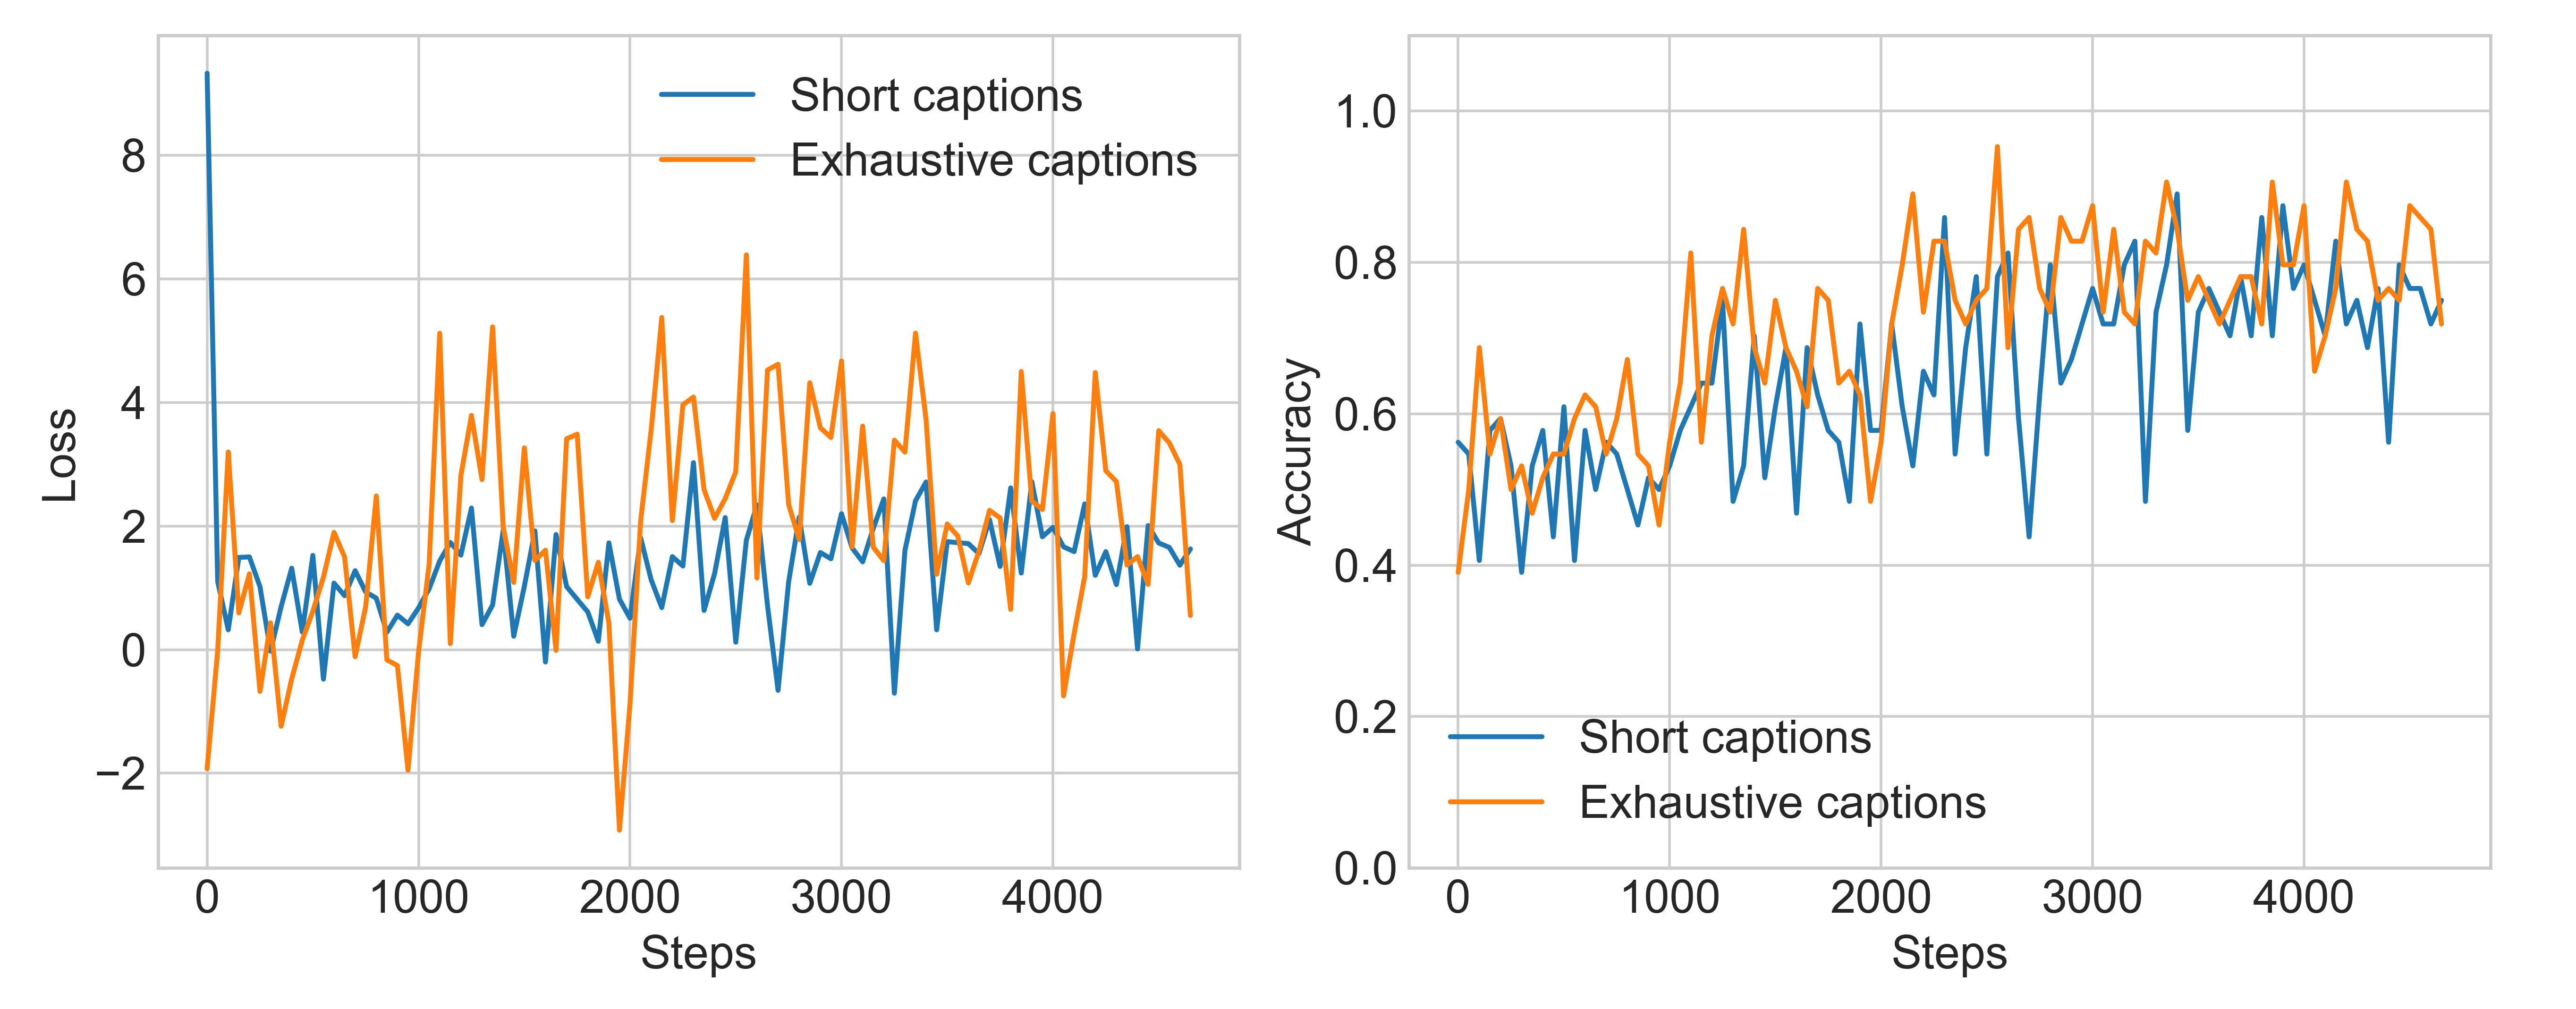
\includegraphics[width=\linewidth]{images/shapes_short_vs_exh_refgame_49_pure_075_similar.png}
%	\caption{Training dynamics on similar image pairs given a dataset with exhaustive captions vs. short captions only.}
%	\label{fig:3dshapes_short_v_exh_similar_losses}
%\end{figure}
%Given the strong effect of length, it does not come surprising that the structural drift of exhaustive captions is higher than of short ones. However, the semantic drift is much more severe for short captions, compared to exhaustive ones, therefore, at least partly supporting \textbf{H10}. 
%\begin{figure}
%	\centering
%	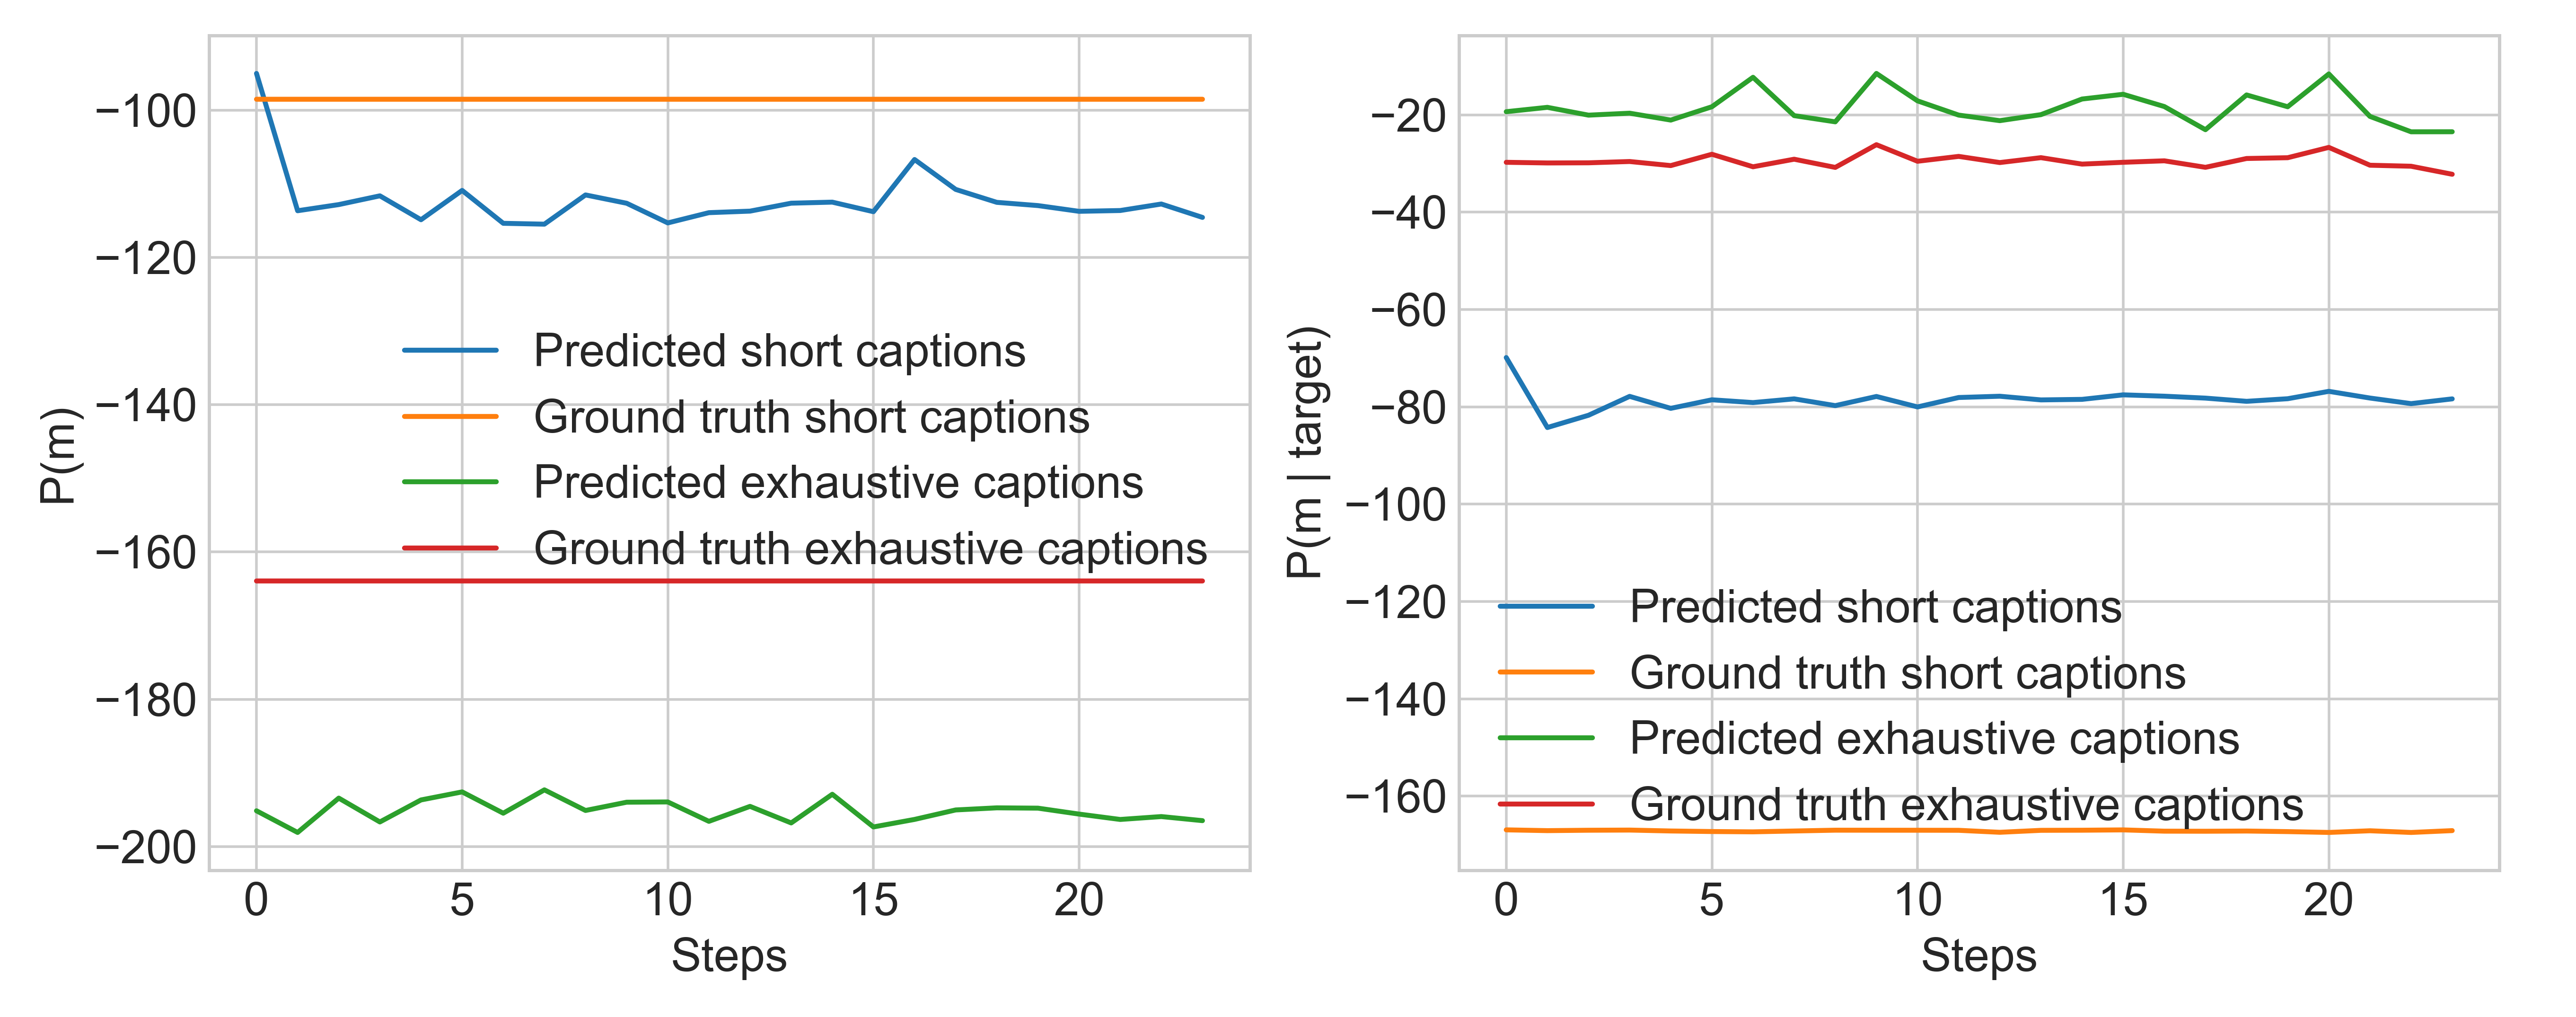
\includegraphics[width=\linewidth]{images/3dshapes_short_vs_exh_structural_semantic_drift_49_pure_075_similar.png}
%	\caption{Language drift metrics computed during training gieven model trained on similar image pairs given a dataset with exhaustive captions vs. short captions only. The drifts were computed on random image pairs for comparability.}
%	\label{fig:3dshapes_short_v_exh_similar_str_sem}
%\end{figure}
\pt{summary of 3Dshapes experiments goes here}
Summarizing the experiments on the 3Dshapes dataset, it was shown that the agents could successfully learn the reference game on this synthetic dataset. Crucially, thir success depended on the similarity of the image pairs. 
The agents were also subject to structural and semantic drift phenomena, although some dynamics differed from the observations in the literature and in the MS COCO experiments, revealing the importance of the nature of visual input, the captions and the action space size (i.e., the vocabulary size) for language drift. It was shown that the capacity of the speaker to be fine-tuned on the task might be dependent on fine-grained differences in the visual input and resulting task-based learning signal \pt{double check strength here}. 
It was shown that the presence of exhaustive annotations was not necessary in order to mitigate language drift, although it might help the speaker to learn to describe most discriminative attributes of the target in complex contexts. On the contrary, dataset statistics like the length of the captions might play a larger role with respect to language drift than the exhaustive content of the annotations.

\section{Language Drift Hypotheses: Discussion}

Experiments described in the previous section addressed several hypotheses regarding language drift in multi-agent reference games and aimed to provide a comprehensive picture as to which factors might influence the strength of different types of drift.
First, results are summarized with respect to the hypotheses (listed in Section~\ref{hypos}), and then a discussion by language drift type is provided.\\
\newline
\textbf{H1:} Confirming expectations, structural drift increased in the baseline experiments on the MS COCO (Section \ref{expt:coco_baseline}) dataset. That is, the log probability under a pretrained LM of the messages generated by the speaker decreased after the agents learned to play the reference game, compared to respective pretrained agents. Additionally to the original expectations, this was the case for all configurations of the structural constraints. In contrast, the hypothesis was not borne out in the 3Dshapes datasets baseline experiment (Section \ref{expt:3dshapes_baseline}) compared to the pretrained speaker. These results indicate that structural constraints might be more effective when the speaker needs to learn a smaller vocabulary like the 3Dshapes one, compared to MS COCO. However, the size of the vocabulary is intertwined with differences in perceptual nature of the images, which might have influenced the strength of the functional training signal, and, therefore, the trade-off with the structural signal.\newline
\textbf{H2:} In contrast to the hypothesized effect, semantic drift was slightly lower in the baseline experiment on MS COCO compared to the pretrained speaker (Section \ref{expt:coco_baseline}). That is, the conditional log probability of the generated message given the target under the pretrained speaker model actually increased. However, the drift was higher for the experiments with $\lambda_s=0.25, \lambda_s=0.5, \lambda_s=1$. In contrast, in line with expectations, semantic drift in the baseline 3Dshapes experiment was higher compared to the pretrained speaker (Section \ref{expt:3dshapes_baseline}). It was additionally the case for the $\lambda_s=0$ experiment. In sum, semantic drift was not as strong as expected; it may be due to the complexity of the reference game and the short task training, such that the effect of task-based optimization was not very pronounced yet and di not lead to tangible drift. \newline
\textbf{H3:} The expectation was that, as the speaker learned to play the reference game, the overlap metrics increase, reflecting that the messages become more discriminative. Against expectations, thel overlap metrics decreased on all experiments compared to the overlaps of the ground truth captions, indicating that, at least on the surface, the difference between the produced messages and the contrast to target versus distractor descriptions decreased, compared to the original difference between the target and distractor ground truth captions. For MS COCO, the discrete overlap was also lower for the baseline experiments than for the pretrained speaker, except for the $\lambda_s = 0, \lambda_s = 0.75$ configurations (Section \ref{expt:coco_baseline}). The continuous overlap was higher than for the pretrained speaker only for the $\lambda_s = 0.25$ configuration.
On 3Dshapes, the discrete overlap was lower on all random pairs experiments than for the pretrained speaker. The continuous overlap was lower in all configurations except for $\lambda_s=0.5$ (Section \ref{expt:3dshapes_baseline}). However, the fact that the overlaps \emph{de}creased may not necessarily be indicative of bad discriminative performance. More specifically, the low discrete overlap value might be due to the fact that the generated captions contain words which were not part of the ground truth caption because, for instance, they refer to features which were not mentioned in the descriptive ground truth captions, but were chosen under discriminative pressure by the trained speaker.\footnote{Thanks to Malte Heyen for the discussion which led to this point.} 
In sum, the data did not provide evidence that the overlap increased as the speakers learned the reference game.\newline
\textbf{H4:} This hypothesis concerned the strength of the structural constraints during training; it was expected that with increasing structural regularization strength, structural and semantic drift would decrease, for both datasets. Varying the structural loss weight on MS COCO (Section \ref{expt:coco_baseline}), it was observed that the structural drift decreased, if anything, with \textit{de}creasing structural loss pressure ($R^2 = -0.878$).\footnote{The Pearson correlation coefficient was computed on the mean validation drift values and structural weights.} Semantic drift also decreased as the structural loss weight decreased ($R^2 = -0.934$). For 3Dshapes (Section \ref{expt:3dshapes_baseline}), structural drift seemed to slightly decrese with increasing structural contraints, but the trend was anecdotal ($R^2=0.028$). By contrast, semantic drift decrease with increasing structural weights was more pronounced ($R^2 = 0.519$). To sum up, the hypothesis was somewhat supported by the data of the 3Dshapes exeriments semantic drift, but not for other aspects. That is, contrary to expectations, language drift was not mitigated by stronger structural constraints, indicating that the reference game training in the different configurations did not override the biases from pretraining. \pt{are there other interpretations available?} \newline
\textbf{H5:} For this hypothesis, the increase in the overlap metrics was expected to be smaller when comparing the pretrained speaker to the speaker trained on similar image pairs, than when comparing the pretrained speaker to the speaker trained on random image pairs. This was expected for both datasets. First, results for discrete overlap are discussed. 
For MS COCO, the increase for random pairs was 0.003 on random pairs and the value decresaed by 1.039 on similar pairs, in favor of the hypothesis (Sections \ref{expt:coco_baseline} and \ref{expt:coco_similar_pairs}). 
For 3Dshapes, the overlap decreased by 0.181 for baseline random pairs. For the fixed features similar pairs with exhaustive captions, when tested on the same test set, it decreased by 2.553. When tested on the different test set it decreased by 3.357 (Section \ref{expt:3dsapes_similar}). Turning to the mixed lengths speaker (Section \ref{expt:3dshapes_short}), the overlap increased by 0.007 on random pairs and decreased on similar pairs (by 1.472 and 0.394, respectively, when tested on same and different test sets). 
Turning to continuous overlap, on MS COCO, the similar pairs overlap increased by 0.001 compared to the increase on random pairs. For 3Dshapes, the overlap decreased compared to the pretrained model on all similar pairs tests, while the random pairs overlap only decreased by 0.001 on mixed length captions.
\pt{random similar pairs on 3Dshapes with exhaustive and short captions, missing for short captions} 
Therefore, in sum, the premise of the hypothesis that the overlap metrics increase after training on the reference game was not supported by the data across the board. It was only the case for discrete overlap on the random pairs MS COCO and mixed captions 3Dshapes baselines and continuous overlap on MS COCO similar pairs. The other speakers' productions overlaps decreased. However, in relative comparison, this speaks in support of the hypothesis, as even for the exhaustive 3Dshapes experiments, the decrease in discrete overlap on similar pairs was much stronger than on random pairs. This decrease was also much stronger for continuous overlap. Overall, this indicates that the functional drift as captured by this metric might not behave as was anticipated and might be dependent oon the length of the productions (as is apparent from the difference in magnitude of values between exhaustive and mixed caption results on 3Dshapes), it does seem to capture functional difficulty of the referential task. Therefore, it may be considered as an approximation of a functional drift metric. However, for more tangible results regarding the continuous overlap, longer training of the embedding layers might be necessary. \newline
\textbf{H6:} Confirming expectations, structural and semeantics drifts were smaller when the speakers were trained against a fixed listener, compared to the jointly trained listeners (Sections \ref{exp:coco_fixed_listener} and \ref{expt:3dshapes_fixed}). More precisely, semantic drift was smaller for fixed listener experiments for both datasets and both structural loss weight configurations (\pt{add averages}). This was also the case for all structural drifts except for the $\lambda_s = 0$ configuration on 3Dshapes, where the dridt was lower with the jointly trained listener. Confirming results from the literature \parencite{lazaridou2020multi}, it is visible that the fixed listener was effective in holding the grounding of the language more constant and thereby alleviating semantic drift. Extending beyond previous results, it even mitigated somewhat the structural drift in the MS COCO experiments, possibly by implicitly enhancing the structural training signal in the large vocabulary space.\newline
\textbf{H9:} %Exhaustive experiments on 3Dshapes (baseline in Section \ref{expt:3dshapes_baseline}, similar pairs on exhaustive captions in Section \ref{expt:3dsapes_similar}, fixed listener in Section \ref{expt:3dshapes_fixed}) versus respective MS COCO experiments (baseline in Section \ref{expt:coco_baseline}, similar pairs in Section \ref{expt:coco_similar_pairs} and fixed listener in Section \ref{exp:coco_fixed_listener}), comparing each fine-tuned speaker to respective baseline.  
This hypothesis posited that the difference in the structural drift between speakers fine-tuned in reference games and the pretrained speakers are smaller for the 3Dshapes experiments compared to the differences of the MS COCO experiments.
Those difference are compared one by one (3Dshapes~vs.~MS COCO) in the following. The average differences in the baseline experiments with varying structural loss weights were 0.340 and 2.824 worse than baseline (Section \ref{expt:3dshapes_baseline} and Section \ref{expt:coco_baseline}); in the similar pairs experiments, they were on average 1.501 better for 3Dshapes and 1.495 worse on MS COCO ( Section \ref{expt:3dsapes_similar} and Section \ref{expt:coco_similar_pairs}); for the fixed listener experiments, they were 0.203 better than pretrained for 3Dshapes and 0.918 worse oon MS COCO (Section \ref{expt:3dshapes_fixed} and Section \ref{exp:coco_fixed_listener}). \pt{these difference values are axactly what i should be computing paired t-tests on. TBD} That is, across the different types of experiments the data supports the hypothesis, indicating that the presence of exhaustive captions during training helps alleviating the structural drift. An additional potential source of the difference remains, however, the different nature of the images (synthetically generated geometric shapes versus real photos) and the difference in the vocabulary sizes the speakers learned (49 tokens versus 4054 tokens). \pt{remove short caps from the 3d computation bc it is about exhaustivity here}  \newline
\textbf{H10:} %3Dshapes on random pairs with exhaustive versus mixed captions (Section \ref{expt:3dshapes_baseline} vs. Section \ref{expt:3dshapes_short}), and on similar pairs (random or fixed features) with exhaustive versus mixed captions (Section \ref{expt:3dsapes_similar} vs Section \ref{expt:3dshapes_short}). 
It was hypothesized that the structural drift is higher for mixed caption experiments compared to exhaustive caption experiments, on all pairs, as measured by the difference in structural drift between fine-tuned and respective pretrained speaker. This expectation was based on the intuition that under a lack of descriptive words, the speaker may resort to structural drift as a strategy for discriminative communication. Furthermore, combined with expectations formulated in \textbf{H5}, increasing the difficulty of the referential task by using similar pairs, it is expected that this difference between exhaustive and mixed caption speakers increases. 
Comparing the baseline experiments on random pairs (Section \ref{expt:3dshapes_baseline}~vs.~Section \ref{expt:3dshapes_short}), this hypothesis was not supported by the data, as the structural drift of the mixed lengths baseline fine-tuned speaker improved compared to the pretrained mixed lengths speaker, while the structural drift of the baseline fine-tuned exhaustive speaker did not change compared to pretrained exhaustive speaker. Comparing structural drifts of these speakers on similar pairs experiments wherein the pairs matched on random features, the exhaustive speaker exhibited structural drift compared to the pretrained one (Section~\ref{expt:3dsapes_similar}). \pt{The comparable experiment on mixed captions is missing}. 
Comparing structural drifts of the exhaustive speaker on similar pairs which matched on fixed features, the drift decreased compared to the pretrained speaker by 2.044 (same test) and 2.229 (different test). For the mixed captions speaker (Section~\ref{expt:3dshapes_short}), the drift increased compared to the pretrained speaker by 0.1 (same test), and decreased by 5.190 compared to pretrained speaker when tested in the different features test set, providing no consistent support for the hypothesis. Taken together, these results indicate that the speaker did not resort to structural drift as a strategy for more successful discriminative communication because of a lack of appropriate descriptive words. She did not do so even given target-distractor pairs which called for more fine-grained discriminative messages. Therefore, one might hypothesize that structural drift is generally rather an artifact of a lack of an appropriate training signal rather than some type of the agent's loophole behavior.
\newline

These results provide an extensive overview of different factors which may influence language drift. Summing up by drift type, it was found that \textbf{structural drift} was best mitigated by the presence of exhaustive captions in the training set, sampled from a not too large action space, and it was dependent on the distribution of lengths of the training sentences. The drift was generally lower for speakers producing shorter messages. For \textbf{semantic drift}, it was found that it was mostly due to speaker-listener co-adaptation, as was shown by the mitigation provided by the fixed listener. Additionally, it was found that semantic drift was much lower when the speaker was trained also on short captions, indicating that grounding was easier to learn from shorter sequences. That is, statistics of the dataset seem to have a larger impact on structural and semantic drifts than content-realted aspects like exhaustivity or the complexity of the scenes or image pairs. \pt{check again} Finally, \textbf{functional drift} measures reflected, first and foremost, the complexity of the referential task, decreasing when the referential task was more complex (like int he similar pairs experiments). Comparing this decrease with the dynamics of test accuracy, it can be seen that the discrete overlap metrics was indicative of the test accuracy, making it a valid task-functional metric \pt{check!!!!} 

In conclusion, the experiments have revealed how strong the effect of the speaker's pretraining is on the downstream performance, and how these effects enter in fine-grained interactions with the environment of the reference game like the nature of the target-distractor pairs, training duration and the length of the available annotations. These results call for much closer attention to training and architectural details in multi-agent communication experiments than is custom in the literature.
% Fixed listener results consistent with \cite{lazaridou2020multi}.
%Note that I did not use the term ``functional'' drift once. Add that in overlap metric discussions.
%If there is no difference between exhaustive and short captions on 3D, it is actually promising - it means that it is not necessary to really have completely exhaustive (almost task-specific) annotations - it is sufficient that the agents saw possible descriptions of all features during pretraining, even when the sentences were short. This means, we can indeed achieve something with RL and interactive learning from experience, it is not all about supervised learning for a given task.

%This seeming insensitivity of the overlap metrics might be due to several reasons. First, due to a lack of comparability to other work, further experiments, e. g., replicating existing work, involving these mterics need to be conducted in order to properly assess their plausibility. Second, the continuous overlap might be subject to vanishing gradients which become too small over the backpropagation steps through time of the message sequence in order to affect the embedding layer \parencite[cf.][]{jaeger2002tutorial}. Finally, it might be the case that generally the training just did not proceed for a sufficient number of epochs for the functional loss to take effect, as literature has argued that REINFORCE based training, especially given large action spaces like the one at hand, is slower to converge \parencite{havrylov2017emergence} \pt{look into Havrylov again: is convergence always in terms of listener performance, or speaker loss too?}.

%Discuss POS analyses in relation to \cite{lee2019countering}.